\documentclass{report}

\usepackage{utdiss2}  		% Dissertation package style file.

\usepackage{array}
\usepackage{amsmath,amssymb,amsfonts,mathrsfs,amsthm}
\usepackage[utf8]{inputenc}
\usepackage{listings}
\usepackage{mathtools}
\usepackage{dsfont}
\usepackage{pdfpages}
\usepackage[textsize=footnotesize,color=green]{todonotes}
\usepackage{algorithm, algorithmic}
\usepackage{bm}
\usepackage{tikz}
\usepackage[normalem]{ulem}

\usepackage{graphicx}
\usepackage{subfigure}
\usepackage{color}
\usepackage{undertilde}
\usepackage[colorlinks = true, filecolor = red, urlcolor = blue, linkcolor = black]{hyperref}
\usepackage{pdflscape}
\usepackage{pifont}
%\usepackage{fullpage}
\setlength\textwidth{6in}
\setlength\textheight{8in}
\setlength\oddsidemargin{0.25in} % LaTeX adds a default 1in to this!
\setlength\evensidemargin{0.25in}
\setlength\topmargin{-0.0in} % LaTeX adds a default 1in to this!
\setlength\headsep{0in}
\setlength\headheight{0in}
\setlength\footskip{1in}

\renewcommand{\topfraction}{0.85}
\renewcommand{\textfraction}{0.1}
\renewcommand{\floatpagefraction}{0.75}

\newcommand{\vect}[1]{\ensuremath\boldsymbol{#1}}
\newcommand{\tensor}[1]{\underline{\vect{#1}}}
\newcommand{\del}{\triangle}
\newcommand{\grad}{\nabla}
\newcommand{\curl}{\grad \times}
\renewcommand{\div}{\grad \cdot}
\newcommand{\ip}[1]{\left\langle #1 \right\rangle}
\newcommand{\eip}[1]{a\left( #1 \right)}
\newcommand{\pd}[2]{\frac{\partial#1}{\partial#2}}
\newcommand{\pdd}[2]{\frac{\partial^2#1}{\partial#2^2}}

\newcommand{\circone}{\ding{192}}
\newcommand{\circtwo}{\ding{193}}
\newcommand{\circthree}{\ding{194}}
\newcommand{\circfour}{\ding{195}}
\newcommand{\circfive}{\ding{196}}

\newcommand{\Reyn}{\rm Re}

\newcommand{\bs}[1]{\boldsymbol{#1}}
\DeclareMathOperator{\diag}{diag}

\newcommand{\equaldef}{\stackrel{\mathrm{def}}{=}}

\newcommand{\tablab}[1]{\label{tab:#1}}
\newcommand{\tabref}[1]{Table~\ref{tab:#1}}

\newcommand{\theolab}[1]{\label{theo:#1}}
\newcommand{\theoref}[1]{\ref{theo:#1}}
\newcommand{\eqnlab}[1]{\label{eq:#1}}
\newcommand{\eqnref}[1]{\eqref{eq:#1}}
\newcommand{\seclab}[1]{\label{sec:#1}}
\newcommand{\secref}[1]{\ref{sec:#1}}
\newcommand{\lemlab}[1]{\label{lem:#1}}
\newcommand{\lemref}[1]{\ref{lem:#1}}

\newcommand{\mb}[1]{\mathbf{#1}}
\newcommand{\mbb}[1]{\mathbb{#1}}
\newcommand{\mc}[1]{\mathcal{#1}}
\newcommand{\nor}[1]{\left\| #1 \right\|}
\newcommand{\snor}[1]{\left| #1 \right|}
\newcommand{\LRp}[1]{\left( #1 \right)}
\newcommand{\LRs}[1]{\left[ #1 \right]}
\newcommand{\LRa}[1]{\left\langle #1 \right\rangle}
\newcommand{\LRc}[1]{\left\{ #1 \right\}}
\newcommand{\tanbui}[2]{\textcolor{blue}{\sout{#1}} \textcolor{red}{#2}}
\newcommand{\Grad} {\ensuremath{\nabla}}
\newcommand{\Div} {\ensuremath{\nabla\cdot}}
\newcommand{\Nel} {\ensuremath{{N^\text{el}}}}
\newcommand{\jump}[1] {\ensuremath{\LRs{\![#1]\!}}}
\newcommand{\uh}{\widehat{u}}
\newcommand{\fnh}{\widehat{f}_n}
\renewcommand{\L}{L^2\LRp{\Omega}}
\newcommand{\pO}{\partial\Omega}
\newcommand{\Gh}{\Gamma_h}
\newcommand{\Gm}{\Gamma_{-}}
\newcommand{\Gp}{\Gamma_{+}}
\newcommand{\Go}{\Gamma_0}
\newcommand{\Oh}{\Omega_h}

\newcommand{\eval}[2][\right]{\relax
  \ifx#1\right\relax \left.\fi#2#1\rvert}

\def\etal{{\it et al.~}}


\def\arr#1#2#3#4{\left[
\begin{array}{cc}
#1 & #2\\
#3 & #4\\
\end{array}
\right]}
\def\vecttwo#1#2{\left[
\begin{array}{c}
#1\\
#2\\
\end{array}
\right]}
\def\vectthree#1#2#3{\left[
\begin{array}{c}
#1\\
#2\\
#3\\
\end{array}
\right]}
\def\vectfour#1#2#3#4{\left[
\begin{array}{c}
#1\\
#2\\
#3\\
#4\\
\end{array}
\right]}
\date{}

\newtheorem{proposition}{Proposition}
\newtheorem{corollary}{Corollary}
\newtheorem{theorem}{Theorem}
\newtheorem{lemma}{Lemma}

\newcommand{\G} {\Gamma}
\newcommand{\Gin} {\Gamma_{in}}
\newcommand{\Gout} {\Gamma_{out}}


%%%%%%%%%%%%%%% End def of new commands %%%%%%%%%%%%%%%%%%%

\author{Jesse Chan}
\address{910 E. 32nd St, Apt.\ 101\\ Austin, Texas 78705}  % Required

\title{A DPG method for compressible flow problems}

\supervisor
	[Leszek Demkowicz]
	{Robert Moser}

\committeemembers
	[Todd Arbogast]
	[Omar Ghattas]
	{Venkat Raman}

\previousdegrees{B.A.}

\oneandonehalfspacequote

\topmargin 0.125in

\makeindex

%%%%%%%%%%%%%%% Start of thesis %%%%%%%%%%%%%%%%%%%

\begin{document}
%\copyrightpage          % Produces the copyright page.
%\commcertpage           % Produces the Committee Certification
\titlepage

\tableofcontents   % Table of Contents will be automatically
                   % generated and placed here.

%\listoftables      % List of Tables and List of Figures will be placed
%\listoffigures     % here, if applicable.


\chapter{Introduction}


\section{Motivations}

Over the last three decades, the use of Computational Fluid Dynamics as an engineering and design tool in design of aircraft has become common.  Wind tunnel experiments are often complemented by computational simulations, and the simulation of off-design conditions.  Great advances have been made in the field since its introduction, especially in areas of meshing, computer architecture, and solution strategies.  Despite this, there still exist many computational limitations in existing CFD methods:  
\begin{itemize}
\item \textbf{Higher order methods :} Higher order methods stand to offer large computational savings through a more efficient use of discrete degrees of freedom.  However, there are very few working higher-order CFD codes in existence, and most higher order methods tend to degrade to first-order accuracy near shocks. The use of higher order codes to solve the steady state equations is even rarer, where convergence of discrete nonlinear steady equations is a tricky issue \cite{BoeingHigherOrder}.  
\item \textbf{Automatic adaptivity :} The use of adaptive meshes is crucial to many CFD applications, where the solution often exhibits very localized sharp gradients and shocks.  Good resolution for such problems under uniform meshes is computationally prohibitive and impractical for most physical regimes of interest.  However, the construction of ``good" meshes is a difficult task, usually requiring a-priori knowledge of the form of the solution.  An alternative to such is the construction of automatically adaptive schemes; such methods usually begin with a coarse mesh and refine based on the minimization of some error.  However, this task is difficult, as the convergence of numerical methods for problems in CFD is notoriously sensitive to mesh quality.  Additionally, the use of adaptivity becomes even more difficult in the context of higher order and $hp$ methods \cite{BoeingHigherOrder}.  
\end{itemize}
Both of these issues are tied to the notion of \emph{robustness}.  We define robustness loosely as the degradation of solution quality with respect

typical physical conditions of interest for the compressible Navier-Stokes equations involve low viscosity/high Reynolds numbers.  

Higher order adaptivity and stability for CFD problems are issues for high Reynolds and Mach numbers. 
\todo{Address the fact that CFD problems have issues of robustness; introduce reasoning that we will study the model problem of convection-diffusion first to better understand this. }

\subsection{Singular perturbation problems and robustness}

Historically, the Galerkin method has been very successfully applied to a broad range of problems in solid mechanics, for which the variational problems resulting from the PDE are symmetric and coercive (positive-definite). It is well known that the finite element method produces optimal or near-optimal results for such problems, with the finite element solution matching or coming close to the best approximation of the solution in the finite element space. However, standard Bubnov-Galerkin methods tend to perform poorly for the class of PDEs known as singular perturbation problems. These problems are often characterized by a parameter that may be either very small or very large in the context of physical problems.  An additional complication of singular perturbation problems is that very often, in the limiting case of the parameter blowing up or decreasing to zero, the PDE itself will change types (e.g.\ from elliptic to hyperbolic).

A canonical example of a singularly perturbed problem is the convection-diffusion equation on domain $\Omega \in \mathbb{R}^3$,
\[
\div \left(\beta u\right) - \epsilon \Delta u = f.
\]
The equation represents the change in the scalar quantity $u$, representing the concentration of a quantity in a given medium, taking into account both convective and diffusive effects. $\beta \in \mathbb{R}^3$ specifies the direction and magnitude of convection, while the singular perturbation parameter $\epsilon$ represents the diffusivity of the medium. In the limit of an inviscid medium as $\epsilon\rightarrow 0$, the equation changes types, from elliptic to hyperbolic, and from second order to first order.

We will illustrate the issues associated with numerical methods for this equation using one dimensional examples.  In 1D, the convection-diffusion equation is
\begin{align*}
\beta u'-\epsilon u'' &= f.
\end{align*}
For Dirichlet boundary conditions $u(0)=u_0$ and $u(1)= u_1$, the solution can develop sharp boundary layers of width $\epsilon$ near the outflow boundary $x=1$. 

\begin{figure}[!h]
\centering
\includegraphics[scale=.4]{figs/GalerkinOscTight.png}
\caption{Oscillations in the 1D finite element solution of the convection-diffusion equation for small diffusion.}
\label{fig:GalerkinOsc}
\end{figure}

The poor performance of the finite element method for this problem is reflected in the bound on the error in the finite element solution --- under the standard Bubnov-Galerkin method with $u\in H^1(0,1)$, we have the bound given in \cite{roos2008robust}:
\[
\|u-u_h\|_\epsilon \leq C \inf_{w_h}\|u-w_h\|_{H^1(0,1)},
\]
for $\|u\|_\epsilon^2 \coloneqq \|u\|_{L^2}^2 + \epsilon \|u'\|_{L^2}^2$, with $C$ independent of $\epsilon$. An alternative formulation of the above bound is 
\[
\|u-u_h\|_{H^1(0,1)} \leq C(\epsilon) \inf_{w_h}\|u-w_h\|_{H^1(0,1)},
\]
where $C(\epsilon)$ grows as $\epsilon\rightarrow 0$. The dependence of the constant $C$ on $\epsilon$ is referred to as a \textit{loss of robustness} --- as the singular perturbation parameter $\epsilon$ decreases, our finite element error is bounded more and more loosely by the best approximation error.  As a consequence, the finite element solution can diverge significantly from the best finite element approximation of the solution for very small values of $\epsilon$.  For example, Figure~\ref{fig:GalerkinOsc} shows an example of how, on a coarse mesh, and for small values of $\epsilon$, the Galerkin approximation of the solution to the convection-diffusion equation with a boundary layer develops spurious oscillations everywhere in the domain, even where the best approximation error is small.  These oscillations grow in magnitude as $\epsilon \rightarrow 0$, eventually polluting the entire solution.  

\section{Goal}

To develop a robust, stable $hp$-adaptive scheme for the steady compressible laminar Navier-Stokes equations in transonic/supersonic regimes.
\todo{FINISH}

\section{Literature review}

For the past half-century, problems in CFD have been solved using a multitude of methods, many of which are physically motivated, and thus applicable only to a small number of problems and geometries. We consider more general methods, whose framework is applicable to different problems in CFD; however, our specific focus will be on the nonlinear shock problems of compressible aerodynamics. Broadly speaking, the most popular general methods include (in historical order) finite difference methods, finite volume methods, and finite element methods.  

\subsection{Finite difference and finite volume methods}

For linear problems, finite difference (FD) methods approximate derivatives based on interpolation of pointwise values of a function.  FD methods were popularized first by Lax, who introduced the concepts of the monotone scheme and numerical flux. For the conservation laws governing compressible aerodynamics, FD methods approximated the conservation law, using some numerical flux to reconstruct approximations to the derivative at a point. Finite volume (FV) methods are similar to finite difference methods, but approximate the integral version of a conservation law as opposed to the differential form. FD and FV have roughly the same computational cost/complexity; however, the advantage of FV methods over FD is that FV methods can be used on a much larger class of discretizations than FD methods, which require uniform or smooth meshes. 

For nonlinear shock problems, the solution often exhibits sharp gradients or discontinuities, around which the solution would develop spurious Gibbs-type oscillations. Several ideas were introduced to deal with oscillations in the solution near a sharp gradient or shock: artificial diffusion, total variation diminishing (TVD) schemes, and slope limiters. However, each method had its drawback, either in terms of loss of accuracy, dimensional limitations, or problem-specific parameters to be tuned \cite{Shu:Lectures}. Harten, Enquist, Osher and Chakravarthy introduced the essentially non-oscillatory (ENO) scheme in 1987 \cite{ENO}, which was improved upon with the weighted essentially non-oscillatory (WENO) scheme in \cite{WENO}. WENO remains a popular choice today for both finite volume and finite difference schemes. Most of these methods can be interpreted as adding some specific artificial diffusion to the given numerical scheme.  We refer to such schemes as \emph{modified equation} methods, as the exact solution no longer satisfies the discrete system due to the presence of additional artificial diffusion.  

Historically, finite volumes and finite difference methods have been the numerical discretizations of choice for CFD applications; the simplicity of implementation of the finite difference method allows for quick turnaround time, and the finite volume method is appealing due to its locally conservative nature and flexibility. More recently, the finite element (FE) method has gained popularity as a discretization method for CFD applications for its stability properties and rigorous mathematical foundations. Early pioneers of the finite element method for CFD included Zienkiewicz, Oden, Karniadakis, and Hughes \cite{ChungCFDBook}.  

\subsection{Stabilized finite element methods}

The finite element/Galerkin method has been widely utilized in engineering to solve partial differential equations governing the behavior of physical phenomena in engineering problems.  The method relates the solution of a partial differential equation (PDE) to the solution of a corresponding variational problem. The finite element method itself provides several advantages --- a framework for systematic mathematical analysis of the behavior of the method, weaker regularity constraints on the solution than implied by the strong form of the equations, and applicability to very general physical domains and geometries for arbitrary orders of approximation. 

Traditionally, instability/loss of robustness in finite element methods has been dealt with using residual-based stabilization techniques.  Given some variational form, the problem is modified by adding to the bilinear form the strong form of the residual, weighted by a test function and scaled by a stabilization constant $\tau$.  The most well-known example of this technique is the streamline-upwind Petrov-Galerkin (SUPG) method, which is a stabilized FE method for solving the convection-diffusion equation using piecewise linear continuous finite elements \cite{SUPG}.  SUPG stabilization not only removes the spurious oscillations from the finite element solution of the convection-diffusion equation, but delivers the best finite element approximation in the $H^1$ norm.  

\subsubsection{SUPG}

The Streamline Upwind Petrov Galerkin (SUPG) method is a stabilization method for $H^1$-conforming finite elements, the idea of which was originally motivated by artificial diffusion techniques in finite differences.  In particular, for the homogeneous 1D convection-diffusion equation, it is possible to recover, under a finite difference method, the exact solution at nodal points by adding an ``exact" artificial diffusion based on the mesh size $h$ and the magnitudes of the convection $\beta$ and the viscosity $\epsilon$.  

The idea of ``exact" artificial viscosity was adapted to finite elements not through the direct modification of the equations, but through the test functions and weighting of the residual.  In particular, finite element and Galerkin methods are often referred to as ``weighted residual" methods, since the starting point of both is to multiply the residual by a particular test, or weighting, function.  Standard Galerkin methods, known as Bubnov-Galerkin methods, simply choose these weighting functions to be the same as the the basis functions used to approximate the solution.  A Petrov-Galerkin method refers to any Galerkin method other than a classical Bubnov-Galerkin method.  

We will introduce the SUPG method at an abstract level for illustrative purposes only.  Further details and perspectives on the SUPG method can be found in \cite{SUPG}, as well as in an upcoming book by Hughes.  The convection-diffusion equation can be written as follows:
\[
Lu = \left(L_{\rm adv} + L_{\rm diff} \right) u = f,
\]
where $L_{\rm adv}u \coloneqq \div \left(\beta u\right)$ is the first order advective operator, and $L_{\rm diff}u \coloneqq \epsilon \Delta u$ is the second-order diffusive operator (then, roughly speaking, $L_{\rm diff} u = 0$).  Let us assume $u$ to be a linear combination of piecewise-linear basis functions $\phi_i, i = 0,\ldots,N$.  The SUPG method is then to solve
\[
\int_\Omega L u v + \int_\Omega \tau \left(L_{\rm adv}v\right)\left( L u - f\right) = \int_\Omega f v 
\]
for where $\tau$ is the SUPG parameter.  For uniform meshes in 1D, $\tau$ is chosen such that, for $f=0$, the matrix system resulting from SUPG is exactly equal to the finite difference system under ``exact" artificial diffusion.  However, unlike the artificial diffusion method, for $f\neq 0$, the SUPG method still delivers optimal stabilization.  In fact, the SUPG finite element solution in 1D is nothing less than the nodal interpolant and the best $H^1$ approximation of the exact solution, as seen in Figure~\ref{fig:SUPG}.

\begin{figure}[!h]
\centering
\subfigure[SUPG and standard FEM solutions]{\includegraphics[scale=.43]{figs/SUPG.png}}
\subfigure[SUPG test function]{\includegraphics[scale=.22]{figs/SUPGtest.png}}
\caption{SUPG and standard Bubnov-Galerkin solutions to the 1D convection-dominated diffusion equation, and a modified SUPG test function (in black) corresponding to a linear basis ``hat" function (in red).  The upwind portion of the element is emphasized, while the downwind portion is decreased.  The magnitude of the discontinuity between the upwind and downwind portion is controlled by the intrinsic timescale parameter $\tau$. }
\label{fig:SUPG}
\end{figure}

The idea of emphasizing the upwind portion of a test function is an old idea, introduced in 1977 by Zienkiewicz et al.\ in \cite{zienkUpwind}.  However, the precise amount of upwinding,\footnote{Insufficient upwinding results in a method which still exhibits oscillations and instabilities, while excessive upwinding leads to an overly diffusive method.} as well as the connection to residual-based stabilization methods, were novel to SUPG.  

The method can be made to ``work" for $p>1$, but the results are not as strong as for linear elements, and there is no clear generalization of SUPG to higher order elements.  Additionally, the stabilization properties of SUPG are weaker in higher dimensions, and the SUPG solution is no longer the $H^1$ best approximation for 2D and 3D problems \todo{find citation}.  Despite these caveats, SUPG is still the most popular stabilization method of choice for convection-diffusion type problems, in both academic and industry applications.  

An important feature of SUPG and other residual-based stabilization techniques that separates it from modified equation methods is the idea of \textit{consistency} --- by adding stabilization terms based on the residual, the exact solution still satisfies the same variational problem (i.e.\ Galerkin orthogonality still holds). Contrast this to the artificial diffusion methods in finite difference and finite volume methods, where a specific amount of additional viscosity is added based on the magnitude of the convection and diffusion parameters: unlike residual-based stabilization schemes, the exact solution to the original equation no longer satisfies the new stabilized formulation.  

This addition of residual-based stabilization terms can be interpreted as a modification of the test functions as well.  For SUPG, the formulation can equivalently be written as
\[
\int_\Omega\left( Lu-f\right) v_i = \int_\Omega f v_i, \quad i = 0,\ldots,N
\]
where $v_i$ is defined as
\[
v_i = \phi_i(x) + \tau L_{\rm adv} \phi_i.  
\]
In other words, the test function $v_i$ is a perturbation of the basis function $\phi_i$ by a scaled advective operator applied to $\phi_i$.  For a linear $C^0$ basis function (the ``hat" function), this naturally leads to a bias in the upwind or streamline direction of the flow $\beta$, as seen in Figure~\ref{fig:SUPG}.  

An important connection can now be made --- stabilization can be achieved by changing the test space for a given problem.  We will discuss in Section~\secref{optimalTest} approaching the idea of stabilization through the construction of \textit{optimal test functions} to achieve optimal approximation properties. 

\subsubsection{DG methods}

Discontinuous Galerkin (DG) methods form a subclass of FEM; first introduced by Reed and Hill in \cite{Reed:73}, these methods were later analyzed by Cockburn and Shu \cite{CockburnShu:DG} and have rapidly gained popularity for CFD problems. Advantages of DG methods include the local conservation property, easily modified local orders of approximation, easy adaptivity in both $h$ and $p$, and efficient parallelizability. Rather than having a continuous basis where the basis function support spans several element cells, DG opts instead for a discontinuous, piecewise polynomial basis, where, like FV schemes, a \emph{numerical flux} facilitates communication between neighboring elements (unlike FV methods, however, there is no need for a reconstruction step). 

The formal definition of the numerical flux (attributed to Peter Lax) on an element boundary is some function of the values on the edges of both the neighboring elements.  An additional reason for the popularity of DG methods is that they can be interpreted as stabilized FE methods through appropriate choices of this numerical flux \cite{Brezzi20063293}. We will illustrate this with the pure convection equation in 1D ---
\begin{align*}
\pd{\left(\beta u\right)}{x} &= f\\
u(0) &= u_0.
\end{align*}
The DG formulation is derived by multiplying by a test function $v$ with support only on a single element $K = [x_K,x_{K+1}]$ and integrating by parts. The boundary term is left alone, such that the local formulation is 
\[
\left.\beta u v\right|_{x_K}^{x_{K+1}} + \int_K -\beta u \pd{v}{x} = \int_K f v,
\]
and the global formulation is recovered by summing up all element-wise local formulations. However, the boundary term in the local formulation is presently ill-defined, as both $u$ and $v$ are dual-valued over element boundaries. Consequently, we make the choice to define the values of $u$ on the boundary (the \emph{traces} of $u$) as
\begin{align*}
u(x_K) \coloneqq u(x_K^-), \quad u(x_{K+1}) \coloneqq u(x_{K+1}^-),
\end{align*}
where $u(x_K^-)$ is the value of $u$ at $x_K$ as seen from the left, and $u(x_K^+)$ the value as seen from the right. Similarly, the traces of $v$ are defined to be
\begin{align*}
v(x_K) \coloneqq v(x_K^+), \quad v(x_{K+1}) \coloneqq v(x_{K+1}^-),
\end{align*}
We will refer to $v(x_K^+)$ as the upwind value of $v(x_K)$, and refer to DG under this specific choice of traces as upwind DG.  This specific choice of $v(x_K)$ as the upwind value is crucial; similarly to SUPG, the upwind DG emphasizes the test function in the direction of convection and changes the way the residual is measured.  As it turns out, the performance of DG for convection-type problems is closely tied to this upwinding --- choosing the value of $v(x_K)$ to be the downwind value $v(x_K^-)$ leads to an unstable method, while choosing $v(x_K)$ to be the average of the upwind and downwind values leads to a DG method with suboptimal stability properties, similar to an $H^1$-conforming continuous Galerkin approximation\cite{Brezzi20063293}.  

Another perspective on the use of the numerical flux in DG methods is that the selection of specific DG fluxes imparts \emph{additional regularity} where needed.  For example, for the pure convection problem, the solution has a distributional derivative in the streamline direction, but is only $L^2$ in the crosswind direction. As a consequence of the regularity of the solution, the boundary trace of the solution is defined only in the direction of convection. The upwind DG method addresses the above issue by choosing the numerical flux to be the upwind flux; in this case, the DG numerical flux can be viewed as imparting additional regularity to the discrete solution than is implied by the continuous setting \cite{DPG1,DPG3}. 

\subsubsection{HDG}

A more recent development in DG methods is the idea of \emph{hybridized} DG (HDG), introduced by Gopalakrishnan and Lazarov \cite{hybridDG}. The hybridized DG framework addresses several criticisms of common DG methods (globally coupled degrees of freedom, complicated/inefficient implementation procedures, suboptimal convergence of approximate fluxes) by identifying degrees of freedom with support only on element edges. Neighboring elements are coupled together only through these degrees of freedom, which can be interpreted as Lagrange multipliers enforcing weak continuity of the trial space. Additionally, HDG methods \todo{add bit about numerical fluxes still used, stabilization params}

\subsubsection{Optimization/NL solvers}

Reference (MIT, Fidkowski)

\todo{Find more nonlinear solvers}

\section{Scope}

This proposal will
\begin{enumerate}
\item Introduce DPG
\item Cover the problem of robustness for model problems
\item Extend results/formulations to nonlinear problems
\item Discuss proposed work
\end{enumerate}

\section{Range of CFD problems}

\begin{figure}[!h]
\centering
\includegraphics[scale=.45]{figs/CFD_tree.pdf}
\caption{A diagram of common CFD problems and their simplifying assumptions.}
\end{figure}

\begin{itemize}
\item Discuss full compressible Navier-Stokes with boundary layers
\item Discuss full compressible Navier-Stokes without boundary layers, connect to Euler (mention Dr Young and Boeing and the IBL connection \cite{BoeingDrela})
\item Discuss model problems
\end{itemize}

\chapter{Range of problems}



\begin{figure}[!h]
\centering
\includegraphics[scale=.45]{figs/CFD_tree.pdf}
\caption{A diagram of common CFD problems and their simplifying assumptions.}
\end{figure}

\section{The compressible Navier-Stokes equations}
\seclab{sec:compNS}

We consider the transient compressible Navier-Stokes equations. For simplicity, we present them in two spatial dimensions. Each equation of the Navier-Stokes system represents the conservation of some physical quantity in the behavior of a fluid inside a general control volume.\footnote{The derivation of the compressible Navier-Stokes equations is a standard result of the Reynolds transport theorem, and can be found in many elementary fluid dynamics books.}

\begin{itemize}
\item{\textbf{Mass conservation}}
\begin{align*}
\pd{\rho}{t} + \div \vecttwo{\rho u }{\rho v} &= 0
\end{align*}

\item{\textbf{Momentum conservation}}
\begin{align*}
\pd{\rho u_1}{t} + \div \left(\vecttwo{\rho u^2+p }{\rho u v} - \boldsymbol \sigma_{1}\right) &=0\\
\pd{\rho u_2}{t} + \div \left(\vecttwo{\rho u v}{\rho v^2+p } - \boldsymbol \sigma_{2}\right) &=0
\end{align*}

\item{\textbf{Energy conservation}}
\begin{align*}
\pd{\rho e}{t} + \div \left(\vecttwo{((\rho e)+p)u}{((\rho e)+p)v} - \boldsymbol \sigma_1 \cdot \boldsymbol u- \boldsymbol \sigma_2 \cdot \boldsymbol u + \vec{q}\right) &=0
\end{align*}
\end{itemize}

We assume our fluid satisfies standard stress laws for $\boldsymbol \sigma$ and $\boldsymbol q$ as well. For viscous stresses $\boldsymbol \sigma$, we assume a Newtonian fluid
\begin{align*}
\sigma_{ij} &= \mu(u_{i,j}+u_{j,i}) + \lambda u_{k,k}\delta_{ij}.
\end{align*}
The coefficients $\lambda$ and $\mu$ are known as the viscosity and bulk viscosity, respectively. The bulk viscosity is often set implicitly through $2\mu + 3\lambda = 0$, known as Stokes' hypothesis. However, since the effect of bulk viscosity can become important for compressible flows, we treat both coefficients separately. In general, $\mu$ and $\lambda$ are functions of temperature, obeying the power law
\[
\mu = \left(\frac{T}{T_0}\right)^\beta,
\]
where $T_0$ is a reference temperature. We choose $\beta = 2/3$ in this case. 

We assume our fluid satisfies Fourier's law, which relates the heat flux $\boldsymbol q$ to the gradient of the temperature through
\begin{align*}
{\boldsymbol q} &= \kappa \grad T,
\end{align*}
where $\kappa$ is generally a function of temperature. 

Finally, we assume our fluid is a thermally and calorically perfect ideal gas. Let $c_p$ and $c_v$ be the specific heats at constant pressure and volume, respectively. Then,
\begin{align*}
p &= (\gamma-1)\rho\iota\\
\iota &= e-\frac{1}{2}(u_1^2+u_2^2)\\
\iota &= c_vT
\end{align*}
where $e$ and $\iota$ are energy and internal energy per unit mass, respectively. 

\todo{write blurb on how comp NS is used - small Re limit}
\todo{write blurb on turbulence}

\subsection{Incompressibility}

\todo{reference Stokes, cite Nate}
\cite{stokesDPG}

\subsection{The linearized Navier-Stokes equations}

The linearized Navier-Stokes equations are the result of small perturbation assumptions applied to the full Navier-Stokes equations. Under such assumptions, the flow is largely uniform, with slight variations that are small compared to the uniform stream velocity. We are interested in the linearized Navier-Stokes equations mainly for mathematical purposes - as the solution to the full Navier-Stokes equations involves a series of solutions for linearized Navier-Stokes, we wish to investigate the behavior of our numerical method with respect to this system.  

\section{The scalar convection-diffusion equation}

The scalar convection-diffusion problem is the prototypical model problem for solving the full Navier-Stokes equations; most stabilized methods consider first the scalar convection-diffusion equation as a test case before attempting a solution of the full Navier-Stokes equations. As discussed previously, an important feature of the convection-diffusion equation is that solutions can develop  boundary layers, a physical feature found in most applications of interest for compressible flow. 

\todo{add perspective on convection-diffusion}

\subsection{Burgers' equation}

The Burgers' equation is physically derived from the incompressible Navier-Stokes equations under the assumption that $\grad p \approx 0$, or that the pressure field is near constant. A feature of the Burgers' equation not present in convection-diffusion is that, due to the presence of the nonlinear term, it can develop shock discontinuities in its solutions in finite time.  The Burgers' equation has also been used to study the phenomenon of turbulence; however, the Burgers equation does not exhibit the chaotic nature and sensitivity to initial conditions that characterizes turbulence as observed in the full and incompressible Navier-Stokes equations. In the scope of this dissertation proposal, Burgers shall be used as to test the extension of our numerical method to nonlinear problems. 

\section{The inviscid case}

The pure convection equation is a result of neglecting the viscous term in the convection-diffusion equation. Physically speaking, these assumptions correspond to the inviscid limit, as well as a particular class of boundary conditions (for example, the wall boundary condition $u = 0$ and prescribed inflow condition may be incompatible in the inviscid limit).  The Euler equations are likewise a result of neglecting the viscous terms in the Navier-Stokes equations.  However, these problems can be ill-posed in the continuous setting.  Take, for example, the vortex problem in Figure~\ref{fig:convCirc}.  A feature of the convection equation is that there is no crosswind diffusion - thus, materials do not mix across streamlines.  However, for the vortex problem, this also implies that the solution on any closed streamline can take any arbitrary value, and is thus undefined.  

\begin{figure}[!h]
\centering
\includegraphics[scale = .22]{figs/convCirc.png}
\caption{Setup for the vortex problem.}
\label{fig:convCirc}
\end{figure}
Formally speaking, the solution to the vortex problem is taken to be the solution to the convection-diffusion equation (with appropriate outflow boundary conditions) as the viscosity tends towards zero, in which case, the solution in the interior would be uniformly zero.  This motivates the need for \emph{artificial viscosity} methods with which to regularize inviscid solutions.  The topic is expansive, and we direct the reader towards \cite{Barter} for a more detailed discussion of past and present artificial viscosity methods.

There is still much interest in solving the inviscid Euler equations in industry --- the full Navier-Stokes models often prove difficult to solve due to the mathematical nature of the equations, and the coupling of the Euler equations with boundary layer models has been successful in simulating many phenomena in compressible flow \cite{BoeingDrela}.  



\chapter{Discontinuous Petrov-Galerkin: a minimum residual method for linear problems}

The Discontinuous Petrov-Galerkin (DPG) method of Demkowicz and Gopalakrishnan was first formulated in \cite{DPG1} as a scheme for the pure convection problem. The method demonstrated promise --- in particular, the method was able to achieve optimal convergence rates for the Peterson problem where standard DG methods were suboptimal. A breakthrough came in \cite{DPG2}, where the concept of locally-computable optimal test functions led to the development of the DPG method in its current form. Soon after, the DPG method was successfully applied to solve the convection-diffusion problem in the small-diffusion limit with $\epsilon = 1e-7$ \cite{DPG2,DPG3}. 

Historically, the name DPG was given by Bottasso, Micheletti, Sacco and Causin to their method for elliptic problems in \cite{BottassoMichelettiSacco02}. The method was then extended to other problems, including convection-diffusion, in \cite{BottassoMichelettiSacco05,CausinSacco05,CausinSaccoBottasso05}. The key point in the method of Bottasso et al.\ was their method of hybridization of fluxes. Whereas HDG methods identify an additional flux unknown on the boundary, the numerical flux coupling neighboring elements together is still typically computed in part by using contributions from interior degrees of freedom on neighboring elements. In the DPG formulation, all numerical fluxes are declared to be independent unknowns, leaving the interior field degrees of freedom completely uncoupled from element to element. This formulation is often referred to as the \emph{ultra-weak} variational formulation. 

Since its inception, the DPG method has been applied to a wide range of problems with great success, including elasticity \cite{DPGElasLocking}, thin body shell problems \cite{DPGElas}, the cloaking problem in electromagnetics \cite{DPGcloak}, both Helmholtz and elastic wave propagation problems \cite{DPG4}, and recently, the linear Stokes equation \cite{stokesDPG}. DPG has also been shown to be a generalization of several successful finite element methods --- comparisons between DPG and standard DG methods can be found in \cite{DPG1}, and more recently, several existing DG methods have been shown to be derivable using the DPG framework \cite{Bui-ThanhDemkowiczGhattas11a,DGDPG}. 

Detailed analysis of the energy setting and well-posedness of DPG has been done for the Poisson and convection-diffusion equations in \cite{analysisDPG}. The well-posedness of DPG has also recently been extended to the large class of Friedrichs systems in \cite{Bui-ThanhDemkowiczGhattas11b}. Significant efforts have also been made in demonstrating the robustness of the DPG method for singular perturbation problems, both in wave propagation \cite{DPG4,DPGwave} and convection-diffusion problems \cite{DPGrobustness, DPGrobustness2}. 

\subsection{Optimal Petrov-Galerkin methods}

\seclab{optimalTest} Petrov-Galerkin methods, in which the test space differs from the trial space, have been explored for over 30 years, beginning with the approximate symmetrization method of Barrett and
Morton~\cite{BARRETT01101981}. The idea was continued with the SUPG method of Hughes, and the characteristic Petrov-Galerkin approach of Demkowicz and Oden~\cite{Demkowicz1986188}, which introduced the
idea of tailoring the test space to change the norm in which a finite element method would converge.

The idea of optimal test functions was introduced by Demkowicz and Gopalakrishnan in \cite{DPG2}.  Conceptually, these optimal test functions are the natural result of the minimization of a residual corresponding to the operator form of a variational equation. The connection between stabilization and least squares/minimum residual methods has been observed previously \cite{GLS}. However, the method in \cite{DPG2} distinguishes itself by measuring the residual of the natural \textit{operator form of the equation}, which is posed in the dual space, and measured with the dual norm, as we now discuss. 	

Throughout this work, we assume that the trial space $U$ and test space $V$ are real Hilbert spaces, and denote $U'$ and $V'$ as the respective topological dual spaces. Let $U_h \subset U$ and $V_h\subset V$ be finite dimensional subsets. We are interested in the following problem: given $l \in V'$, find $u_h \in U_h$  such that 
%\begin{equation}
%\eqnlab{variationEq}
%\left\{
%  \begin{array}{l}
%    \text{Given } l \in V', \text{ find } u_h \in U_h  \text{ such that} \\ 
%    b(u_h,v_h) = l(v_h), \quad \forall v_h\in V_h,
%  \end{array}
%  \right.
%\end{equation}
\begin{align}
b(u_h,v_h) &= l(v_h), \quad \forall v_h\in V_h, \eqnlab{variationEq}
\end{align}
where $b\LRp{\cdot,\cdot}: U \times V \to \mbb{R}$ is a continuous
bilinear form.  $U$ is chosen to be some trial space of approximating functions, but $V_h$ is as of yet unspecified. Throughout this work, we suppose the variational problem \eqnref{variationEq} to be well-posed. 

We can identify a unique operator $B:U\rightarrow V'$ such that
\[
\langle Bu,v\rangle_V \coloneqq b(u,v), \quad u\in U, v\in V
\]
with $\LRa{\cdot, \cdot}_V$ denoting the duality pairing between $V'$ and $V$, to obtain the operator form of the continuous variational problem
\begin{equation}
\eqnlab{dualEq}
Bu = l \quad \text{in } V'.
\end{equation}
In other words, we can represent the continuous form of our variational equation
\eqnref{variationEq} equivalently as the operator equation \eqnref{dualEq} with values in the
dual space $V'$.  This motivates us to consider the conditions under which the solution to \eqnref{variationEq} is the solution to the minimum residual problem in $V'$ 
\[
u_h = \underset{u_h\in U_h}{\arg\min}\, J(u_h),
\]
where $J(w)$ is defined for $w\in U$ as 
\[
J(w) = \frac{1}{2}\|Bw-l\|_{V'}^2 \coloneqq\frac{1}{2} \sup_{v\in V\setminus\{0\}} \frac{| b(w,v)-l(v)|^2}{\nor{v}_V^2}.
\]
For convenience in writing, we will abuse the notation $\sup_{v \in V}$ to denote $\sup_{v\in V\setminus\{0\}}$ for the remainder of this work.

Let us define $R_V: V \to V'$ as the Riesz map, which identifies
elements of $V$ with elements of $V'$ by 
\[
\langle R_V v,\delta
v\rangle_V \coloneqq(v, \delta v)_V, \quad \forall \delta v \in V.
\]
Here, $(\cdot, \cdot)_V$ denotes the
inner product in $V$. As $R_V$ and its inverse, $R_V^{-1}$, are both
isometries, e.g.\ $\|f\|_{V'} = \|R_V^{-1} f\|_V, \forall f \in V'$, we
have
\begin{equation}
\eqnlab{minimization}
\min_{u_h\in U_h} J(u_h) = \frac{1}{2}\left\|Bu_h-l\right\|_{V'}^2 =  \frac{1}{2}\left\|R_V^{-1}(Bu_h-l)\right\|_V^2.
\end{equation}
The first order optimality condition for \eqnref{minimization} requires
the G\^ateaux derivative to be zero in all directions $\delta u \in U_h$, i.e.,
\begin{align*}
\left(R_V^{-1}(Bu_h-l),R_V^{-1}B\delta u\right)_V = 0, \quad \forall \delta u \in U. 
\end{align*}
We define, for a given $\delta u \in U$, the corresponding {\em optimal test function} $v_{\delta u}$
\begin{equation}
\eqnlab{optv}
v_{\delta u} \coloneqq R_V^{-1}B\delta u \quad  \text{in } V.
\end{equation} 
The optimality condition then becomes
\[
 \langle Bu_h-l, v_{\delta u}\rangle_V = 0, \quad \forall \delta u \in U
\]
which is exactly the standard variational equation in
 \eqnref{variationEq} with $v_{\delta u}$ as the test functions. We can define the optimal test space $V_{\rm opt} \coloneqq \{v_{\delta u} \text{ s.t. } \delta u\in U\}$. Thus, the solution of the variational problem \eqnref{variationEq} with test space $V_h = V_{\rm opt}$ minimizes the residual in the dual norm $\nor{Bu_h-l}_{V'}$. This is the key idea behind the concept of optimal test functions. 

Since $U_h \subset U$ is spanned by a finite number of basis functions $\LRc{\varphi_i}_{i=1}^N$, \eqnref{optv} allows us to compute (for each basis function) a corresponding optimal test function $v_{\varphi_i}$. The collection $\LRc{v_{\varphi_i}}_{i = 1}^N$ of optimal test functions then forms a basis for the optimal test space.  In order to express optimal test functions defined in \eqnref{optv} in a more familiar form, we take  $\delta u = \varphi$, a generic basis function in $U_h$, and rewrite \eqnref{optv} as
\[
R_Vv_{\varphi} = B\varphi, \quad \text{in } V',
\]
which is, by definition, equivalent to
\[
\LRp{v_\varphi,\delta v}_V = \LRa{R_Vv_\varphi,\delta v}_{V}=
\LRa{B\varphi, \delta v}_V = b\LRp{\varphi,\delta v}, \quad
\forall \delta v \in V.
\]
%% Now, let us define the \textit{trial-to-test} operator $T =
%% R_V^{-1}B$, which, by \eqnref{optv}, maps a trial function $\delta u$
%% to its corresponding \textit{optimal} test function $v = T\delta u$.
%% On the other hand,
As a result, optimal test functions can be determined by solving the auxiliary
variational problem
\begin{equation}
\eqnlab{optvVar}
\left(v_\varphi,\delta v\right)_V = b(\varphi,\delta v), \quad \forall
\delta v \in V.
\end{equation}
However, in general, for standard $H^1$ and $H({\rm div})$-conforming finite element methods, test functions are continuous over the entire domain, and hence solving variational problem \eqnref{optvVar} for each optimal test function requires a global operation over the entire mesh, rendering the method impractical. A breakthrough came through the development of
discontinous Galerkin (DG) methods, for which basis functions are
discontinuous over elements. In particular, the use of discontinuous
test functions $\delta v$ reduces the problem of determining global 
optimal test functions
in \eqnref{optvVar} to local problems that can be solved in an
element-by-element fashion.

We note that solving \eqnref{optvVar} on each element exactly is
infeasible since it amounts to inverting the Riesz map $R_V$ exactly.
Instead, optimal test functions are approximated using the standard
Bubnov-Galerkin method on an ``enriched" subspace $\tilde{V} \subset
V$ such that $\dim(\tilde{V}) > \dim(U_h)$ elementwise \cite{DPG1, DPG2}. In this
document, we assume the error in approximating the optimal test functions
is negligible, and refer to the work in \cite{practicalDPG} for
estimating the effects of approximation error on the performance of DPG.

It is now well known that the DPG method
delivers the best approximation error in the ``energy norm" --- that is
\cite{Bui-ThanhDemkowiczGhattas11a, DPG2,DPG4} 
\begin{equation}
\eqnlab{optimalError}
\nor{u-u_h}_{U,E} = \inf_{w\in U_h} \nor{u-w}_{U,E},
\end{equation}
where the energy norm $\|\cdot \|_{U,E}$ is defined for a function $\varphi \in U$ as
\begin{equation}
\eqnlab{energyNorm} \|\varphi\|_{U,E} \coloneqq \sup_{v\in V}
\frac{b(\varphi,v)}{\|v\|_V} = \sup_{\nor{v}_V = 1} b(\varphi,v) =
\sup_{\nor{v}_V = 1} \LRa{B\varphi,v}_V = \nor{B\varphi}_{V'} =
\nor{v_\varphi}_V,
\end{equation}
where the last equality holds due to the isometry of the Riesz map
$R_V$ (or directly from \eqnref{optvVar} by taking the supremum). An
additional consequence of adopting such an energy norm is that,
without knowing the exact solution, the energy error $\|u-u_h\|_{U,E}$ can
be determined by computing $\|v_{u-u_h}\|_V$ from the following
identity
\[
\left(v_{u-u_h},\delta v\right)_V = b(u-u_h,\delta v) = l\LRp{\delta
v} - b(u_h,\delta v).
\]
This is simply a consequence of the minimum-residual nature of DPG; the energy error is simply the norm of the  residual in $V'$. 

Practically speaking, this implies that the DPG method is not only discretely stable, but delivers the \emph{best approximation in the energy norm} on any mesh. In particular, the stability and optimality of DPG apply naturally to higher order adaptive meshes, where discrete stability is often an issue. 

\subsection{Ultra-weak variational formulation}
\seclab{abstractUweak}

The naming of the discontinuous Petrov-Galerkin method refers to the fact that the method is a Petrov-Galerkin method, and that the test functions are specified to be discontinuous across element boundaries. There is no specification of the regularity of the trial space, and we stress that the idea of DPG is not inherently tied to a single variational formulation \cite{Bui-ThanhDemkowiczGhattas11a}. 

In most of the DPG literature, however, the discontinuous Petrov-Galerkin method refers to the combination of the concept of locally computable optimal test functions in Section \secref{optimalTest} with the so-called ``ultra-weak formulation" \cite{DPG1,DPG2,DPG3,DPG4,DPGElas,DBLP:journals/procedia/NiemiCC11}. Unlike the previous two sections in which we studied the general equation \eqnref{variationEq} given by abstract bilinear and linear forms, we now consider a concrete instance of \eqnref{variationEq} resulting from an ultra-weak formulation for an abstract first-order system of PDEs $Au = f$. Additionally, from this section onwards, we will refer to DPG as the pairing of the ultra-weak variational formulation with the concept of locally computable optimal test functions. 

We begin by partitioning the domain of interest $\Omega$ into $\Nel$ non-overlapping elements $K_j, j = 1,\hdots,\Nel$ such that $\Oh = \cup_{j=1}^\Nel K_j$ and $\overline{\Omega} = \overline{\Omega}_h$. Here, $h$ is defined as $h= \max_{j\in \LRc{1,\hdots,\Nel}}\text{diam}\LRp{K_j}$.  We denote the mesh ``skeleton" by $\Gh = \cup_{j=1}^\Nel \partial K_j$; the set of all faces/edges $e$, each of which comes with a normal vector ${n}_e$. The internal skeleton is then defined as $\Gamma^0_h = \Gh \setminus \partial \Omega$. If a face/edge $e \in \Gh$ is the intersection of $\partial K_i$ and $\partial K_j$, $i \ne j$, we define the following jumps:
\[
\jump{v} = \text{sgn} \LRp{{n}^-}v^- + \text{sgn} \LRp{{n}^+}v^+, \quad
\jump{\tau \cdot n} = {n}^-\cdot \tau^- + {n}^+\cdot\tau^+,
\]
where
\[
\text{sgn}\LRp{{n}^{\pm}} =
\left\{
\begin{array}{ll}
1 & \text{if } {n}^{\pm} = {n}_e \\
-1 & \text{if } {n}^\pm = -{n}_e
\end{array}
\right..
\]
For $e$ belonging to the domain boundary $\partial \Omega$, we define
\[
\jump{v} = v, \quad
\jump{\tau \cdot n} = {n}_e\cdot \tau.
\]
Note that we allow arbitrariness in assigning ``-'' and ``+'' quantities to the adjacent elements $K_i$ and $K_j$.

The ultra-weak formulation for $Au = f$ on $\Oh$, ignoring boundary
conditions for now, reads
\begin{equation}
\eqnlab{uweak}
b\left(\left(u, \widehat{u}\right),v\right) \coloneqq \langle \widehat{u}, \jump{v}
\rangle_{\Gh} - (u,A_h^*v)_{\Oh}= \LRp{f,v}_{\Oh},
\end{equation}
where we have denoted $\LRa{\cdot,\cdot}_{\Gh}$ as the duality
pairing on $\Gh$, $\LRp{\cdot,\cdot}_{\Oh}$ the $L^2$-inner
product over $\Oh$, and $A_h^*$ the formal adjoint resulting from
element-wise integration by parts.  Occasionally, for simplicity in
writing, we will ignore the subscripts in the duality pairing and
$L^2$-inner product if they are $\Gh$ and $\Oh$. Both the
inner product and formal adjoint are understood to be taken
element-wise. Using the ultra-weak formulation, the regularity
requirement on solution variable $u$ is relaxed, that is, $u$ is now
square integrable for the ultra-weak formulation \eqnref{uweak} to be
meaningful, instead of being (weakly) differentiable.  The trade-off
is that $u$ does not admit a trace on $\Gh$ even though it did
originally. Consequently, we need to introduce an additional new
``trace'' variable $\widehat{u}$ in \eqnref{uweak}, that is defined only on
$\Gh$.

The energy setting is now clear; namely,
\[
u\in L^2\LRp{\Oh} \equiv L^2(\Omega), \quad v\in V=D(A^*_h), \quad
\widehat{u}\in \gamma(D(A)),
\]
where $D(A_h^*)$ denotes the broken graph space corresponding to $A_h^*$,
and $\gamma(D(A))$ the trace space (assumed to exist) of the graph space of
operator $A$. The first discussion of the well-posedness of DPG with the ultra-weak formulation can be found in \cite{analysisDPG}, where the proof is presented for the Poisson and convection-diffusion equations. A more comprehensive discussion of the abstract setting for DPG with the ultra-weak formulation using the graph space, as well as a more general proof of well-posedness, can be consulted in \cite{Bui-ThanhDemkowiczGhattas11b}. 

\subsection{Choices of test and trial norms}
\seclab{energyPair}

A clear property of the energy norm defined by \eqnref{energyNorm} is that the trial norm $\nor{\cdot}_{U,E}$ is induced by a given test norm. However, the reverse relationship holds as well; for any trial norm, the test norm that induces such a norm is recoverable through duality. We have a result, proved in \cite{Bui-ThanhDemkowiczGhattas11a}: assuming, for simplicity, that the bilinear form $b(u,v)$ is definite, given any norm $\nor{\cdot}_{U}$ on the trial space $U$, for $\varphi \in U$, we can represent $\nor{\varphi}_{U}$ via
\[
\nor{\varphi}_{U} = \sup_{v \in V}\frac{b\LRp{w,v}}{\nor{v}_{V,U}}.
\]
where $\nor{v}_{V,U}$ is defined through
\[
\nor{v}_{V,U} = \sup_{w \in U}\frac{b\LRp{w,v}}{\nor{w}_{U}}.
\]
%In other words, the norm $\nor{\cdot}_V$ in $V$ can be recovered using the energy norm $\nor{\cdot}_{U,E}$ in $U$, and vice versa. 

In particular, given two arbitrary norms $\nor{\cdot}_{U,1}$ and $\nor{\cdot}_{U,2}$ in $U$
such that $\nor{\cdot}_{U,1} \le c \nor{\cdot}_{U,2}$ for some constant
$c$, they generate two norms $\nor{\cdot}_{V,U,1}$ and
$\nor{\cdot}_{V,U,2}$ in $V$ defined by
\[
\nor{v}_{V,U,1} \coloneqq \sup_{w \in U}\frac{b\LRp{w,v}}{\nor{w}_{U,1}}, \quad
\text{and }\nor{v}_{V,U,2} \coloneqq \sup_{w \in U}\frac{b\LRp{w,v}}{\nor{w}_{U,2}},
\]
such that $\nor{\cdot}_{V,U,1}$ and $\nor{\cdot}_{V,U,2}$ induce
$\nor{\cdot}_{U,1}$ and $\nor{\cdot}_{U,2}$ as energy
norms in $U$, respectively. That is,
\[
\|\varphi\|_{U,1} = \sup_{v\in V}
\frac{b(\varphi,v)}{\|v\|_{V,U,1}}, \quad \text{and }\|\varphi\|_{U,2} = \sup_{v\in V}
\frac{b(\varphi,v)}{\|v\|_{V,U,2}}.
\]

A question that remains to be addressed is to establish the relationship
between $\nor{\cdot}_{V,U,1}$ and $\nor{\cdot}_{V,U,2}$, given that
$\nor{\cdot}_{U,1} \le c \nor{\cdot}_{U,2}$. But this is
straightforward since we have
\begin{align*}
 \| v \|_{V,U,2} = \sup_{u \in U} \frac{b\left(w,v\right)}{\left\|
  w \right\|_{U,2}} \le c\sup_{w \in U} \frac{b\left(w,v\right)}{\left\| w
  \right\|_{U,1}} = c\| v \|_{V,U,1}.
\end{align*}
Consequently, a stronger energy norm in $U$ will generate a weaker
norm in $V$ and vice versa. In other words, to show that an
energy norm $\nor{\cdot}_{U,1}$ is weaker than another energy norm
$\nor{\cdot}_{U,2}$ in $U$, one simply needs to show the reverse inequality on the
corresponding norms in $V$, that is, $\nor{\cdot}_{V,U,1}$ is stronger
than $\nor{\cdot}_{V,U,2}$.

From now on, unless otherwise stated, we will refer to $\nor{\cdot}_{V,U}$ as the test norm that induces a given norm $\nor{\cdot}_U$. Likewise, we will refer $\nor{\cdot}_{U,V}$ as the trial norm induced by a given test norm $\nor{\cdot}_V$. In this work, for simplicity of exposition, we shall call a pair of norms in $U$ and $V$ that induce each other as an {\em energy norm pairing}.

From the discussion above of energy norm and test norm pairings, we know that specifying either a test norm or trial norm is sufficient to define an energy pairing. We now derive and discuss two important energy norm pairings, the first of which begins by specifying the canonical norm in $U$ and inducing a test norm on $V$. The second pairing begins instead by specifying the canonical norm on $V$ under the ultra-weak formulation \eqnref{uweak} and inducing an energy norm on the trial space $U$.

We begin first with the canonical norm in $U$. Since $\uh \in \gamma\LRp{D\LRp{A}}$, the standard norm for $\uh$ is
the so-called minimum energy extension norm defined as
\begin{equation}
\eqnlab{MEnorm}
\|\widehat{u}\| = \inf_{w\in D\LRp{A},
  \left.w\right|_{\Gh}=\widehat{u}} \|w\|_{D\LRp{A}}.
\end{equation}
The canonical norm for the group variable $\LRp{u,\uh}$ is then given by
\[
\|\left(u,\widehat{u}\right)\|_U^2 = \|u\|^2_{\L} + \|\widehat{u}\|^2,
\]
Applying the Cauchy-Schwarz inequality, we arrive at
\[
b\LRp{\LRp{u,\uh},v} \le \nor{\LRp{u,\uh}}_U \nor{v}_{V,U},
\]
where
\[
\nor{v}_{V,U}^2 = \|A_h^*v\|_{\L}^2
+\left(\sup_{\widehat{u} \in \gamma\LRp{D\LRp{A}}} \frac{\LRa{ \widehat{u},
  \jump{v} }_{\Gh}}{\|\widehat{u}\|}\right)^2.
\]

On the other hand, since $v \in D\LRp{A^*_h}$, the canonical norm for
$v$ is the broken graph norm: 
\[
\nor{v}_V^2 =  \|A_h^*v\|_{\L}^2 + \nor{v}_{\L}^2.
\]
Using the Cauchy-Schwarz inequality again, we obtain
\[
b\LRp{\LRp{u,\uh},v} \le \nor{\LRp{u,\uh}}_{U,V} \nor{v}_{V},
\]
where
\begin{equation}
\eqnlab{inducedQuasi}
\nor{\LRp{u,\uh}}_{U,V}^2 = \nor{u}_{\L}^2
+\sup_{v \in D\LRp{A_h^*}} \frac{\LRa{\widehat{u},
  \jump{v}}_{\Gh}^2}{\|v\|_V^2},
\end{equation}

Using the framework developed in \cite{Bui-ThanhDemkowiczGhattas11a},
one can show that both pairs $\LRp{\nor{\LRp{u,\uh}}_U,
  \nor{v}_{V,U}}$ and $\LRp{\nor{\LRp{u,\uh}}_{U,V}, \nor{v}_{V}}$ are
energy norm pairings in the sense discussed in Section
\secref{energyPair}. That is, the canonical norm $\nor{\LRp{u,\uh}}_U$
in $U$ induces (generates) the norm $\nor{v}_{V,U}$ in $V$, while the
canonical norm $\nor{v}_V$ in $V$ induces (generates) the energy norm
$\nor{\LRp{u,\uh}}_{U,V}$ in $U$. In the DPG literature \cite{DPG4}, $\nor{v}_{V,U}$ is known as the {\em optimal test norm},
while $\nor{v}_{V}$ is known as the {\em quasi-optimal test norm}.

\begin{figure}[!h]
\centering
\begin{tabular}{l c c}
Trial norm & & Test norm \\
\hline
$\boxed{\|u\|^2_{\L} + \|\widehat{u}\|^2}$ & $\Longrightarrow$  & $\|A_h^*v\|_{\L}^2
+\left(\sup_{\widehat{u}} \frac{\LRa{ \widehat{u},
  \jump{v} }_{\Gh}}{\|\widehat{u}\|}\right)^2$ \\
%\hline
%Quasi-optimal trial norm & & Canonical test norm \\
%\hline
$\nor{u}_{\L}^2+\sup_{v } \left(\frac{\LRa{\widehat{u},
  \jump{v}}_{\Gh}}{\|v\|_V}\right)^2$ &  $\Longleftarrow$ & $\boxed{\|A_h^*v\|_{\L}^2 + \nor{v}_{\L}^2}$
\end{tabular}
\caption{A summary of the derivation of test/trial norm pairings; we begin with the boxed norm on either the trial or test space, and induce the norm on the other space through duality. The optimal \textit{test} norm is naturally derived by beginning with the canonical norm on the trial space, while the quasi-optimal \textit{trial} norm is derived from beginning with the canonical norm on the test space.}
\end{figure}

The canonical norm $\nor{\LRp{u,\uh}}_U$ in $U$ provides a good
balance between the standard norms on the field $u$ and the flux
$\uh$ \cite{DPG4}. As a result, if the induced norm $\nor{v}_{V,U}$ (namely, the
optimal test norm) is used to compute  optimal test functions in
\eqnref{optvVar}, the finite element error in the canonical norm is the
best in the sense of \eqnref{optimalError}. 

Unfortunately, the optimal test norm is non-localizable due to the presence of the jump term $\jump{v}$.\footnote{A localizable norm can be written as $\nor{v}_{V(\Oh)} = \sum_{K\in\Oh} \nor{v}_{V(K)},$ where $\nor{v}_{V(K)}$ is a norm over $K$.} Since the jump terms couple elements together, the evaluation of the jump terms requires contributions from all the elements in the mesh. Consequently, solving for an optimal test function
amounts to inverting the Riesz map %, defined on the left sideof \eqnref{optvVar}, 
over the entire mesh $\Oh$, making the optimal test norm impractical.

On the other hand, the quasi-optimal test norm $\nor{v}_V$, namely the canonical norm in $V$, \textit{is} localizable, and hence practical. However, it's worth noting the difference between the induced energy norm $\nor{\LRp{u,\uh}}_{U,V}$ and the canonical norm in $U$; under the induced norm $\nor{\LRp{u,\uh}}_{U,V}$ there is no natural interpretation for the norm in which the error in the flux variable $\uh$ is measured. 

Using a variant of the quasi-optimal test norm, numerical results show that the DPG method appears to provide a ``pollution-free" method without phase error for the Helmholtz equation \cite{DPG4}, and analysis of the pollution-free nature of DPG is currently under investigation. Similar results have also been obtained in the context of elasticity \cite{DPGElas} and the linear Stokes equations \cite{Camellia}. On the theoretical side, the quasi-optimal test norm has been shown to yield a well-posed DPG methodology for the Poisson and convection-diffusion equations \cite{analysisDPG}. More recently, this theory has been generalized to show the well-posedness of DPG under the quasi-optimal test norm for the large class of Friedrichs' type PDEs \cite{Bui-ThanhDemkowiczGhattas11b}.  


\chapter{A robust DPG method for convection-diffusion}

\section{DPG formulation for convection-diffusion}

\seclab{sec:modelSec}
The remainder of this chapter focuses on the convection-diffusion problem using the abstract theory that we
have discussed so far. In particular, we shall use the DPG method based on the ultra-weak formulation with optimal test functions to solve this model problem and analyze its behavior with respect to $\epsilon$. 
Our goal is to show the robustness of the method with respect to $\epsilon$, and demonstrate its usefulness as  a numerical approach to solving singular-perturbed problems. 

The convection-diffusion problem is given on a domain
$\Omega \subset \mathbb{R}^d$ with boundary $\pO \equiv \Gamma$
\begin{equation}
\div (\beta u) - \epsilon\Delta u = f  \in \L \label{primal},
\end{equation}
which can be cast into the first order form on the group variable
$\LRp{u,\sigma}$ as
\begin{equation}
\eqnlab{CDstrong}
A \LRp{u,\sigma} \coloneqq \LRs {
\begin{array}{c}
\div (\beta u - \sigma) \\ \frac{1}{\epsilon}\sigma - \grad u
\end{array}} = \LRs{
\begin{array}{c}
f \\ 0
\end{array}
}.
\end{equation}
Using the abstract ultra-weak formulation developed in Section
\secref{abstractUweak} for the first order system of PDEs \eqnref{CDstrong} we
obtain
\begin{align*}
b\left(\left(u,\sigma, \widehat{u}, \widehat{f}_n\right),
\left( v, \tau \right)\right) = \left(u,\div \tau - \beta \cdot \grad
v\right)_{\Oh} + \left(\sigma, \epsilon^{-1} \tau + \grad v\right)_{\Oh} - \LRa{
\jump{\tau\cdot n}, \widehat{u} }_{\Gh} + \LRa{ \widehat{f}_n,
  \jump{v} }_{\Gh},
\end{align*}
where $\LRp{v, \tau}$ is the group test function. It should be pointed
out that the divergence and gradient operators are understood to act
element-wise on test functions $\LRp{v, \tau}$ in the broken graph
space $ D\LRp{A_h^*} \coloneqq  H^1(\Oh) \times H({\rm div}, \Oh)$, but
globally as usual on conforming test functions, i.e.\ $ \LRp{v, \tau}
\in  H^1(\Omega) \times H({\rm div}, \Omega)$. It follows that the
canonical test norm can be written as
\[
\|\left(v, \tau\right)\|_V^2 = \|\left(v, \tau\right)\|_{H^1(\Oh) \times H({\rm div},\Oh)}^2
= \sum_{K\in \Oh} \|\left(v, \tau\right)\|_{H^1(K) \times H({\rm
    div},K)}^2,
\]
where
\[
\|\left(v, \tau \right)\|_{H^1(K) \times H({\rm div},K)}^2 =
\|v\|_{L^2(K)}^2 + \|\grad v\|_{L^2(K)}^2 + \|\tau\|_{L^2(K)}^2 +
\|\div \tau\|_{L^2(K)}^2.
\]

In order to define the proper norm on the trial space, boundary
conditions need to be specified. We begin by splitting the boundary
$\Gamma$ as follows
\begin{align*}
\Gamma_{-} &\coloneqq \{x\in \Gamma; \beta_n(x) < 0\}, \quad {\rm
  (inflow)}\\ \Gamma_{+} &\coloneqq \{x\in \Gamma; \beta_n(x) > 0\},
\quad {\rm (outflow)}\\ \Gamma_{0} &\coloneqq \{x\in \Gamma;
\beta_n(x) = 0\},
\end{align*}
where $\beta_n \coloneqq \beta \cdot n$.
Previous work in \cite{DPGrobustness} adopted Dirichlet boundary
conditions everywhere on $\Gamma$.  
%and we could obtain the robustness only with special weighted norms in which the weight varied spatially. 
We employ instead the inflow
condition of Hesthaven \etal \cite{Hesthaven96astable}, where we set
\[
\beta_n u - \sigma_n  = u_0, \quad \text{on } \Gm,
\]
instead of $\beta_n u = u_0$. The former resembles the latter
as $\epsilon$ approaches zero\footnote{For our model problem, as for many problems of interest in computational fluid dynamics, we expect $\grad u$ to be small near the inflow, and that the solutions to \eqref{primal} using $\beta_n u - \sigma_n = f_n = u_0$ on $\Gamma_-$ will converge to that using $u=u_0$ on $\Gamma_-$  for sufficiently small $\epsilon$.}; however, the latter induces a more ``well-behaved" adjoint problem than the former, which, as we will discuss, affects the performance of DPG. 

On the outflow boundary, we apply standard homogeneous Dirichlet boundary conditions
\[
u = 0, \quad \text{on } \Gp.
\]
This work is intended to act as an extension of work presented by Heuer and Demkowicz in \cite{DPGrobustness}. The primary focus of this chapter is to analyze the DPG method and extend previous results under this new choice of inflow boundary conditions. The difference in the performance of DPG under both new and old boundary conditions is connected to the difference in the adjoint problems induced under each boundary condition. The secondary contribution of this work will be to analyze the performance of DPG under a new mesh-dependent test norm. 

\subsection{Norms on $U$}

With the above boundary conditions at hand, the ultra-weak formulation
\eqnref{uweak} can be fitted in the abstract form \eqnref{variationEq}
as
\begin{align*}
b\left(\left(u,\sigma, \widehat{u}, \widehat{f}_n\right), \left( v,
\tau\right)\right) &= \left(u,\div \tau - \beta \cdot \grad
v\right)_{\Oh} + \left(\sigma, \epsilon^{-1} \tau + \grad
v\right)_{\Oh} \\
&- \LRa{ \jump{\tau\cdot n}, \widehat{u} }_{\Gh
  \setminus \Gp} + \LRa{ \widehat{f}_n, \jump{v} }_{\Gamma_h \setminus
  \Gm} =  \left(f, v\right) -
\LRa{ u_0, v }_{\Gamma_-} = l\left(\left(v, \tau\right)\right),
\end{align*}
which, after using the setting in Section \secref{abstractUweak},
suggests the following trial space (see \cite{analysisDPG, Bui-ThanhDemkowiczGhattas11b} for details):
\begin{align*}
u, \sigma \in \L, \quad \text{and } \LRp{\uh,\fnh} \in
\gamma\LRp{D\LRp{A}} \subset \gamma\LRp{  H^1(\Omega) \times
H({\rm div}, \Omega)} = H^{\frac{1}{2}}\left(\Gh\right) \times H^{-\frac{1}{2}}\left(\Gh\right).
\end{align*}
The space for $u$ and $\sigma$ are simply scalar and vector $L^2$ spaces over $\Omega$, while the space for $\left(\uh,\fnh\right)$ is the trace space of the graph space of the operator $A$ subject to the boundary conditions.

The minimum energy extension norm \eqnref{MEnorm} now reads
\begin{align*}
\|\widehat{u}\| &= \inf_{w\in H^1(\Omega),
  \left.w\right|_{\Gamma_+}=0, \left.w\right |_{\Gh\setminus
    \Gamma_+ } = \widehat{u}} \|w\|_{H^1(\Omega)}, \\ \|\widehat{f}_n\|
&= \inf_{q\in H({\rm div},\Omega), \left.q\cdot n\right|_{\Gamma_-}=
  0, \left. q\cdot n \right |_{\Gh\setminus
    \Gamma_-} = \widehat{f}_n}
\|q\|_{H({\rm div},\Omega)}.
\end{align*}
As a result, the canonical norm on $U$ is given by
\[
\left\|\left(u,\sigma,\widehat{u},\widehat{f}_n\right)\right\|_U^2 = 
\|u\|_{L^2(\Oh)}^2 + \|\sigma\|_{L^2(\Oh)}^2 +
\|\widehat{u}\|^2 + \|\widehat{f}_n\|^2.
\]

\subsection{Norms on $V$}

%We will denote $\|\cdot \| = \|\cdot\|_{L^2}$ for all functions defined on $\Oh$. 
As $\tau \in H({\rm div},\Oh)$ and $v \in H^1(\Oh)$, we will
construct norms on $v$ and $\tau$ 
which are equivalent to the canonical $H^1(K) \times H({\rm div},K)$
norm over a single element
\[
\|\left(v,\tau\right)\|_{H^1(K) \times H({\rm div},K)}^2 =
\|v\|_{L^2(K)}^2 + \|\grad v\|_{L^2(K)}^2 + \|\tau\|_{L^2(K)}^2 +
\|\div \tau\|_{L^2(K)}^2.
\]
The squared norm over the entire triangulation $\Oh$ is defined to be the squared sum of contributions from each element
\[
\|\left(v,\tau\right)\|_{H^1(\Oh) \times H({\rm div},\Oh)}^2
= \sum_{K\in \Oh} \|\left(v,\tau\right)\|_{H^1(K) \times H({\rm
    div},K)}^2.
\]
The exact norms that we will specify on $V$ will be determined later. 

The norms on the skeleton $\Gh$ for $v$ and $\tau$ are defined by duality from the bilinear form
\begin{align*}
\left\|\jump{\tau\cdot n}\right\| &= \left\|\jump{\tau\cdot n}\right\|_{\Gh \setminus \Gamma_+} \coloneqq \sup_{w\in H^1(\Omega), \left.w\right|_{\Gamma_+} = 0} \frac{\langle \jump{\tau \cdot n}, w\rangle}{\|w\|_{H^1(\Omega)}},\\
\left\|\jump{v}\right\|&=\left\|\jump{v}\right\|_{\Gh^0 \cup \Gamma_+} \coloneqq \sup_{\eta\in H({\rm div},\Omega), \left.\eta\cdot n\right|_{\Gamma_- \cup \Gamma_0} = 0} \frac{\langle \jump{v}, \eta\cdot n\rangle}{\|\eta\|_{H({\rm div},\Omega)}}.
\end{align*}

\subsection{Approximability of the quasi-optimal test norm}
%\textcolor{blue}{need to define what we mean by robustness. perharps the best place is in the introduction}
An obvious choice for the test norm would be the quasi-optimal norm; it is the canonical test norm, and DPG has been shown to be well-posed and robust under such an optimal test norm for a large class of problems \cite{DPGrobustness,Bui-ThanhDemkowiczGhattas11b, stokesDPG}. However, computations with the quasi-optimal test norm for convection-diffusion problems turn out to be quite problematic for small diffusion and coarse meshes.  

For convection-diffusion, the quasi-optimal test norm is 
\[
\|\left(v,\tau\right)\|_V^2 = \| \div \tau - \beta \cdot \grad v
\|_{L^2}^2 + \| \epsilon^{-1} \tau + \grad v \|_{L^2}^2 +
\|v\|_{L^2}^2 + \|\tau\|_{L^2}^2.
\]
%We note that the optimal test norm will automatically guarantee the
%robust bound $\|\left(\tau, v\right)\|_V \leq \|u\|_{L^2}$.
Use of this norm for the convection-diffusion problem is difficult --- since the problem \eqnref{optvVar} for optimal test functions is local, we can transform the problem over a single element $K$ to the reference element $\widehat{K}$ and show that it is equivalent to a reaction-diffusion system, with diffusion parameter $\frac{\epsilon}{|K|}$, where $|K|$ is the element measure \cite{DBLP:journals/procedia/NiemiCC11}. We refer to the inverse of this parameter $\frac{|K|}{\epsilon}$ as the element Peclet number $\rm Pe$. For a coarse mesh and small diffusion parameter $\epsilon$, we will have a large element Peclet number, and optimal test functions under the quasi-optimal test norm will develop strong boundary layers of width $\rm Pe$, as seen in Figure~\ref{fig:optTestBoundary}.

In the application of DPG in \cite{DPG1,DPG2,DPG3,DPG4}, the approximation of optimal test functions is done using polynomial enrichment. We search for the solution to \eqnref{optvVar} in the enriched test space $\tilde{V} \approx \prod_{K} P^{p+\Delta p}(K)$, where $p$ is the polynomial order of the trial space on a given element $K$.\footnote{$V$ is only \emph{approximately} equal to the space $\prod_{K} P^{p+\Delta p}(K)$. In practice, $V$ is constructed using locally $H^1$-conforming and Raviart-Thomas elements of appropriate order.}  In other words, optimal test functions are approximated element-by-element using polynomials whose order is $\Delta p$ more than the local order of approximation.  Under this scheme, the error in approximation of test functions is tied to the effectiveness of the $p$-method.  Unfortunately, for problems with boundary layers --- including the approximation of test functions under the quasi-optimal test norm --- the $p$-method performs very poorly. As a result of this poor approximation, the numerical solutions of the convection-dominated diffusion equation under DPG using the quasi-optimal test norm tend to be of poor quality, and do not exhibit all the proven properties of DPG (for example, the energy error may increase after mesh refinement, even though, by virtue of DPG delivering a best approximation, the energy error for a coarse mesh must be greater than or equal to the energy error for a finer mesh).  We conclude that the error in approximation of optimal test functions using simple polynomial enrichment pollutes and ruins the performance of DPG under the quasi-optimal test norm. 

\begin{figure}[!h]
\centering
\includegraphics[scale=.25]{figs/opt.png}
\caption{$v$ and $\tau$ components of the 1D optimal test functions corresponding to the flux $\widehat{f}_n$ on the right-hand side of a unit element for $\epsilon = 0.01$. The solution has been obtained using automatic $hp$-adaptivity driven by the test norm with the error tolerance set at 1\%.}
\label{fig:optTestBoundary}
\end{figure}

The difficulty in using the quasi-optimal test norm for convection-diffusion is perplexing at first, considering that the quasi-optimal norm has yielded excellent results for the Helmholtz equation and other wave propagation problems.  The difference between the two problems lies in the fact that, for wave propagation problems, the mesh size tends to be on the order of the wavenumber $k$ --- the singular perturbation parameter. Transforming the variational problem using the quasi-optimal test norm for wave propagation yields smooth optimal test functions that are approximated much more accurately using only polynomials over the reference element. Typically, the wavenumbers $k$ of physical interest are $O(100)$ with respect to a unit domain. The corresponding finite element problems will typically be solved on meshes containing approximately $O\!\left(k^d\right)$ elements in $\mathbb{R}^d$, well within the range of a computationally tractable simulation. However, for convection diffusion problems, the relevant range of $\epsilon$ for physical problems can be as small as $1e-7$. Solving on under-resolved meshes is thus unavoidable, and the approximability of optimal test functions must be addressed in order to take advantage of the properties of DPG.

Resolving such boundary layers present in test functions under the quasi-optimal test norm has been investigated numerically using specially designed (Shishkin) subgrid meshes by Niemi, Collier, and Calo in
\cite{DBLP:journals/procedia/NiemiCC11}.  However, even with Shishkin meshes, the approximation of optimal test functions under the quasi-optimal norm is far more expensive and complex to implement than approximation of test functions using a simple $p$-enriched space for $V$. We therefore aim instead to design a test norm that does not induce boundary layers, but still delivers good approximation results over a range of $\epsilon$.  

\subsection{Analysis of a DPG test norm}
\seclab{sec:testNormSec}
We are interested in computing DPG optimal test functions for the convection-diffusion equation with very small values of $\epsilon$; due to the difficulty of approximating optimal test functions, we conclude that the use of the quasi-optimal test norm is infeasible towards this goal. 

However, if we naively choose a test norm that does not generate boundary layers, the performance of DPG may be adversely affected. For example, if $\|\left(v,\tau\right)\|_V^2 = \|v\|_{H^1(\Omega_h)}^2 + \|\tau\|^2_{H({\rm div},\Omega_h)}$, the $H^1(\Omega_h)\times H({\rm div},\Omega_h)$ norm, then the corresponding test functions will be smooth and free of boundary layers; however, the performance of DPG will provide approximations which worsen in quality as $\epsilon$ becomes very small \cite{DPG3,DPGrobustness}. 

Our goal is to construct a test norm that compromises between performance of DPG and approximability of test functions.  This test norm should not produce boundary layers in the optimal test functions, but still induce an energy norm that yields good approximation properties for small $\epsilon$. We note that, even under the quasi-optimal norm, the norms on the flux and trace variables will likely depend on $\epsilon$. Thus, we aim to construct a test norm for which the DPG method will be robust in $\epsilon$ with respect to the \emph{field variables}. 

For now, we discuss the steps necessary to analyze the performance of DPG with respect to a non-canonical test norm. We require a priori that the test norm has separable $\tau$ and $v$ components --- in other words, that there are no terms in the test norm that couple $\tau$ and $v$ together. Problem \eqnref{optvVar} then decouples, such that the components of the vector-valued test function $\left(v,\tau\right)$ can be solved for independently of each other. The decoupled variational problems are no longer systems but scalar equations in $\tau$ and $v$, for which it is easier to conclude whether or not there are boundary layers in the solutions (the avoidance of boundary layers in the test norm will be discussed in more detail in Section~\ref{sec:num_exp}, which describes our numerical experiments). \textbf{This will ensure that the resulting DPG method does not suffer from approximation errors in the optimal test functions}.

We begin with the following test norm:
\[
\left\|\left(v,\tau\right)\right\|^2_V \coloneqq \|v\|_{L^2}^2 + \epsilon\|\grad v\|_{L^2}^2 + \|\beta \cdot \grad v\|_{L^2}^2  + \frac{1}{\epsilon}\|\tau\|_{L^2}^2 + \|\div \tau\|_{L^2}^2.
\]
The use of this norm is problematic for practical computations; we will discuss the reasons why and present a modification of it in Section~\secref{sec:meshDep}. 

We can see how this norm will differ from the canonical $H^1(\Omega_h)\times H({\rm div},\Omega_h)$ norm: the clearest difference is the fact that the gradient in the streamline direction is $O(1)$, while the full gradient is $O(\sqrt{\epsilon})$, so that, in our test norm, the streamline gradient of $v$ will be emphasized over the full gradient of $v$ for small $\epsilon$. 

The choice of this test norm is implied by the mathematics of the adjoint problem. Roughly speaking, necessary conditions for the performance of DPG to not degenerate as $\epsilon \rightarrow 0$ are derived through analysis of specific test functions. For example, if $u$ is the first $L^2$ component of the solution to the variational problem defined in Section~\secref{sec:modelSec}, by choosing $(v,\tau) \in H^1(\Omega) \times H({\rm div},\Omega)$ such that 
\begin{align*}
\div \tau - \beta \cdot \grad v &= u \\
\frac{1}{\epsilon} \tau - \grad v &= 0,
\end{align*}
we have
\[
 \nor{u}_{L^2}^2 = b\left(\left(u,\sigma,\widehat{u},\widehat{f}_n\right),\left(v,\tau\right)\right) \leq \nor{\left(u,\sigma,\widehat{u},\widehat{f}_n\right)}_{U,V} \nor{\left(v,\tau\right)}_V,
\]
and we recover the $L^2$ norm of $u$ from the bilinear form.

Let $\|a\| \lesssim \|b\|$ denote an $\epsilon$-independent bound; specifically, that $\|a\| \leq C\|b\|$ for a constant $C$ independent of $\epsilon$. Consequently, if for any $u\in L^2(\Oh)$, $\nor{\left(v,\tau\right)}_V\lesssim \nor{u}_{L^2}$, then dividing through by $\nor{u}_{L^2}$ gives the bound
\[
 \nor{u}_{L^2} \lesssim \nor{\left(u,\sigma,\widehat{u},\widehat{f}_n\right)}_E.
\]
In other words, there is the guarantee that the $L^2$ error in $u$ is at least robustly bounded from above by the energy error. Then, if the energy error (which DPG minimizes) approaches zero, the $L^2$ error in $u$ will as well. The same exercise can be repeated for the stress $\sigma$, as well as the flux variables $\widehat{u}$, $\widehat{f}_n$. 

This methodology gives constraints on the quantities found in the test norm; any quantity present in $\nor{\left(v,\tau\right)}_V$ must be shown to be bounded from above independently of $\epsilon$ by the load of the adjoint problem. However, showing this simply amounts to showing \textit{standard energy estimates} for $H^1$ and $H({\rm div})$-conforming finite elements. A more detailed discussion on the reasoning behind the construction of test norms can be found in \cite{DPGrobustness}. 

The second step will be to \textbf{show the equivalence of the energy norm to explicit norms on $U$}. Since we do not generally have a closed form expression for the DPG energy norm, we seek to understand the behavior of DPG by finding a norm on $U$ to which the DPG energy norm is equivalent. Since $\left(u,\sigma,\widehat{u},\widehat{f}_n\right)\in U$ is a group variable from a tensor product space, we construct norms on $U$ through the combination of norms on $u$, $\sigma$, $\widehat{u}$, and $\widehat{f}_n$. Specifically, we use the norm on $U$ 
\begin{equation}
\left\| \left(u,\sigma,\widehat{u},\widehat{f}_n\right)\right \|_{U}^2 \coloneqq \|u\|^2 + \|\sigma\|^2 + \left\|\widehat{u}\right\|^2 + \left\|\widehat{f}_n\right\|^2.
\end{equation}
For equivalence between norms, two constants are specified. However, since this norm on $U$ is a norm on four separate variables, we can specify not just two but eight equivalence constants.\footnote{Sharper estimates are attainable if these constants are allowed to vary over the mesh $\Oh$. See Section~\ref{sec:main_bounds} for a discussion.} In order to simplify analysis, we phrase this equivalence statement in an alternative form. 

Let $\nor{\cdot}_E \coloneqq \nor{\cdot}_{U,V}$, the energy norm induced by the test norm described above. We seek the bound of $\nor{\cdot}_E$ from above and below:
\[
\left\| \left(u,\sigma,\widehat{u},\widehat{f}_n\right)\right \|_{U,1} \lesssim  \left\| \left(u,\sigma,\widehat{u},\widehat{f}_n\right)\right \|_E \lesssim \left\| \left(u,\sigma,\widehat{u},\widehat{f}_n\right)\right \|_{U,2},
\]
where both $\|\cdot\|_{U,1}$ and $\|\cdot\|_{U,2}$ are defined as scaled combinations of the norms on $u, \sigma, \widehat{u}$, and $\widehat{f}_n$
\begin{equation}
\eqnlab{uNorms}
\left\| \left(u,\sigma,\widehat{u},\widehat{f}_n\right)\right \|_{U,i}^2 \coloneqq \left(C_u^i\|u\|\right)^2 + \left(C_\sigma^i\|\sigma\|\right)^2 + \left(C_{\widehat{u}}^i\|\widehat{u}\|\right)^2 + \left(C_{\widehat{f}_n}^i\|\widehat{f}_n\|\right)^2,\quad i = 1,2
\end{equation}
Our goal is to explicitly derive the equivalence constants 
%$C^1_u,\ldots, C^1_{\widehat{f}_n}$ and $C^2_u,\ldots, C^2_{\widehat{f}_n}$ 
that define the norms $\|\cdot\|_{U,1}$ and $\|\cdot\|_{U,2}$ respectively, taking into account any dependency on $\epsilon$. To do so, we need a relation between trial norms on $U$ and test norms on $V$.

Recall from Section~\secref{energyPair} that every test norm induces a corresponding trial norm, and vice versa. Let $\|\cdot\|_{U,1} \simeq \|\cdot\|_{U,2}$ mean that the norms $\|\cdot\|_{U,1}$ and $\|\cdot\|_{U,2}$ are equivalent, with equivalence constants independent of $\epsilon$. By equivalence of finite dimensional norms and the discussion in Section~\secref{energyPair} on the duality between test norms/energy norms, the norms \eqnref{uNorms} on $U$ induce the equivalent test norms on $\left(v,\tau\right) \in H^1(\Oh)\times H({\rm div},\Oh)$
\begin{align*}
\left\|\left(v,\tau\right)\right\|_{V,{U,i}} &\simeq \sup_{\left(u,\sigma,\widehat{u},\widehat{f}_n\right)\in U}\frac{b\left(\left(u,\sigma,\widehat{u},\widehat{f}_n\right),\left(v,\tau\right)\right)}{C_u^i\|u\| + C_\sigma^i\|\sigma\| + C_{\widehat{u}}^i\|\widehat{u}\|+ C_{\widehat{f}_n}^i\|\widehat{f}_n\|}\\
&= \sup_{\left(u,\sigma,\widehat{u},\widehat{f}_n\right)\in U}\frac{\left(u,\div \tau - \beta \cdot \grad v\right) + \left(\sigma, \epsilon^{-1} \tau + \grad v\right) - \langle \jump{\tau_n}, \widehat{u} \rangle_{\Gamma_-\cup \Gh^0} + \langle \widehat{f}_n, \jump{v} \rangle_{\Gamma_+ \cup \Gh^0}}{C_u^i\|u\| + C_\sigma^i\|\sigma\| + C_{\widehat{u}}^i\|\widehat{u}\|+ C_{\widehat{f}_n}^i\|\widehat{f}_n\|}\\
& \simeq \frac{1}{C_u^i}\|g\| + \frac{1}{C_\sigma^i}\|f\| + \frac{1}{C_{\widehat{u}}^i}\sup_{\widehat{u}\neq 0, \left.\widehat{u}\right|_{\Gamma_+} = 0} \frac{\langle \jump{\tau\cdot n}, \widehat{u}\rangle}{\|\widehat{u}\|} +\frac{1}{C_{\widehat{f}_n}^i}\sup_{\widehat{f}_n\neq 0, \left.\widehat{f}_n\right|_{\Gamma_-}=0}\frac{\langle \widehat{f}_n, \jump{v}\rangle}{\|\widehat{f}_n\|},
\end{align*}
where $f$ and $g$ are defined element-wise over $\Oh$ as 
\begin{align*}
g &\coloneqq \div \tau - \beta \cdot \grad v\\
f &\coloneqq \epsilon^{-1}\tau + \grad v.
\end{align*}
By definition of the norms on the quantities defined on the skeleton $\Gh$, this gives the characterization of the induced test norm 
\[
\|\left(v,\tau\right)\|_{V,{U,i}} \simeq \frac{1}{C_u^i}\|g\| + \frac{1}{C_\sigma^i}\|f\| + \frac{1}{C_{\widehat{u}}^i}\|\jump{\tau\cdot n}\| + \frac{1}{C_{\widehat{f}_n}^i}\|\jump{v}\|, \quad i = 1,2.
\]
We can now use this relation to compare different norms on $U$ by comparing their induced norms on $V$ (recall that showing a robust inequality between two norms on $U$ is equivalent to showing the robust \textit{reverse} inequality in the induced norms on $V$). Namely, we can show the bound of $\nor{\cdot}_{U,1} \lesssim \nor{\cdot}_E$ by showing the bound $\nor{\left(v,\tau\right)}_{V,U,1} \gtrsim \nor{\left(v,\tau\right)}_{V}$, and likewise for $\nor{\cdot}_E \lesssim \nor{\cdot}_{U,2}$. 

Since the techniques used to show such bounds are more involved, we break the procedure up into two steps:
\begin{enumerate}
\item{}Decompose test functions $(v,\tau)$ into three separate, more easily analyzable components (Section~\ref{sec:strategy2}).
\item{}Derive adjoint estimates (Section~\ref{sec:strategy3}).
\end{enumerate}

\subsubsection{Decomposition into analyzable components}
\label{sec:strategy2}

Having reduced the problem of comparing norms on $U$ to the comparison of norms on $V$, we break the analysis of $\left(v,\tau\right) \in V$ into the analysis of three subproblems.  Define the decomposition
\[
\left(v,\tau\right) = \left(v_0,\tau_0\right) + \left(v_1,\tau_1\right) + \left(v_2,\tau_2\right),
\]
where $\left(v_1,\tau_1\right)$ satisfies 
\begin{align*}
\epsilon^{-1}\tau_1 + \grad v_1 &= 0 ,\\
\div \tau_1 - \beta\cdot \grad v_1 &=  \div \tau - \beta\cdot \grad v = g, 
\end{align*} 
and $\left(v_2,\tau_2\right)$ satisfies
\begin{align*}
\epsilon^{-1}\tau_2 + \grad v_2 &= \epsilon^{-1}\tau + \grad v = f, \\
\div \tau_2 - \beta\cdot \grad v_2 &= 0.
\end{align*}
Both $(v_1,\tau_1), (v_2,\tau_2) \in H({\rm div}; \Omega)\times H^1(\Omega)$ are understood to satisfy these relations in a conforming sense over the domain $\Omega$; however, the divergence of $\tau$ and gradient of $v$ on the right hand side are still understood to be taken in an element-wise fashion. 

We will additionally require both $\left(v_1,\tau_1\right), \left(v_2,\tau_2\right)$ to satisfy the adjoint homogeneous boundary conditions
\begin{align}
\tau_i\cdot n &= 0, \quad \text{on }\Gamma_- \label{bc_1}\\
v_i &= 0, \quad \text{on } \Gamma_+ \label{bc_2}
\end{align}
for $i = 1, 2$. The selection of $H({\rm div}, \Omega)\times H^1(\Omega)$ conforming test functions satisfying the specific boundary conditions above removes the contribution of the jump terms over the skeleton $\Gh$ in the bilinear form, allowing us to analyze field terms in the induced test norms separately from  the boundary/jump terms. 

Finally, by construction, $\left(v_0,\tau_0\right) \in H^1(\Oh) \times H({\rm div},\Oh)$ must satisfy 
\begin{align*}
\epsilon^{-1}\tau_0 + \grad v_0 &= 0\\
\div \tau_0 - \beta\cdot \grad v_0 &= 0
\end{align*}
with jumps
\begin{align*}
\jump{v_0} &= \jump{v}, \quad \text{on }\Gh^0\\
\jump{\tau_0 \cdot n} &= \jump{\tau \cdot n}, \quad \text{on }\Gh^0.
\end{align*}
and boundary conditions
\begin{align*}
v_0 &= v, \quad \text{on } \Gamma_+ \\
\tau_0 \cdot n &= \tau \cdot n, \quad \text{on } \Gamma_-\cup \Gamma_0. 
\end{align*}
Notice that the evaluation the bilinear form $b\left(\left(u,\sigma,\widehat{u},\widehat{f}_n\right),\left(v,\tau\right)\right)$ with each specific test functions returns only one part of the bilinear form. Furthermore, by choosing the proper loads $g = u$ and $f=\sigma$, we can recover from the bilinear form the norms of $u$ and $\sigma$ (as described in Section~\secref{sec:testNormSec}), as well as the norms on $\widehat{u}$, and $\widehat{f}_n$.\footnote{To recover the norms on $\widehat{u}$, and $\widehat{f}_n$, the loads $f$, and $g$ must be zero, and the jumps of the test function $(v,\tau)$ must be chosen specifically.}

We have now decomposed an arbitrary test function $\left(\tau,v\right)$ into a discontinuous contribution and two continuous contributions.  Recall that our goal is to show the robust bound from above and below of the DPG energy norm by $\|\cdot \|_{U,1}$ and $\|\cdot \|_{U,2}$:
\[
\left\| \left(u,\sigma,\widehat{u},\widehat{f}_n\right)\right \|_{U,1} \lesssim  \left\| \left(u,\sigma,\widehat{u},\widehat{f}_n\right)\right \|_E \lesssim \left\| \left(u,\sigma,\widehat{u},\widehat{f}_n\right)\right \|_{U,2}.
\]

Under the duality of trial and test norms and the decomposition of test functions $\left(\tau,v\right) \in V$ into $\left(\tau_0,v_0\right), \left(\tau_1,v_1\right)$, and $\left(\tau_2,v_2\right)$, the above bound is equivalent to bounding each component 
\begin{align*}
\|\left(v,\tau\right)\|_{V,U,1} &\gtrsim \sum_{i=0}^2\|\left(v_{i},\tau_{i}\right)\|_V \gtrsim \|\left(v,\tau\right)\|_{V,U,2}.
%\|\left(v,\tau\right)\|_{V,1} &\lesssim \|\left(v_{1},\tau_{1}\right)\|_V \lesssim \|\left(v,\tau\right)\|_{V,2}\\
%\|\left(v,\tau\right)\|_{V,1} &\lesssim \|\left(v_{2},\tau_{2}\right)\|_V \lesssim \|\left(v,\tau\right)\|_{V,2}
\end{align*}
Bounding $\|\left(v_0,\tau_0\right)\|$ requires the use of techniques first developed in \cite{analysisDPG} and adapted to convection-diffusion in \cite{analysisDPG} and \cite{DPGrobustness}. However, since $\left(\tau,v\right) \in H({\rm div}, \Omega)\times H^1(\Omega)$, the bound from above of test functions $\|\left(v_{1},\tau_{1}\right)\|_V$ and $\|\left(v_{2},\tau_{2}\right)\|_V$ is reduced to proving classical error estimates for the adjoint equations
\begin{align*}
\epsilon^{-1}\tau_1 + \grad {v_1} &= 0 \\
\div {\tau_1} - \beta\cdot \grad {v_1} &=  g, \\
\left.\tau_1\cdot n\right|_{\Gamma_-} &= 0, \\
\left.v_1\right|_{\Gamma_+} &= 0.
\end{align*} 
and 
\begin{align*}
\epsilon^{-1}\tau_2 + \grad {v_2} &= f \\
\div {\tau_2} - \beta\cdot \grad {v_2} &= 0, \\
\left.\tau_2\cdot n\right|_{\Gamma_-} &= 0, \\
\left.v_2\right|_{\Gamma_+} &= 0.
\end{align*} 
More generally, we can analyze the adjoint equations
\begin{align}
\epsilon^{-1}\tau + \grad {v} &= f \label{adjoint1}\\
\div {\tau} - \beta\cdot \grad {v} &= g, \label{adjoint2}
\end{align}
for arbitrary data $f, g\in L^2({\Omega})$ and boundary conditions $\jump{\tau\cdot n}_{\Gamma_-} = 0$ and $\jump{v}_{\Gamma_+} = 0$.  In other words, we want to analyze the stability properties of the adjoint equations by deriving bounds of the form $\|\left(v_1,\tau_1\right)\|_V\lesssim \|g\|_{L^2}$ and $\|\left(v_2,\tau_2\right)\|_V \lesssim \|f\|_{L^2}$.  

%An alternate interpretation of the above decomposition is that each component $(v_i,\tau_i)$ of the decomposition corresponds to a term in the bilinear form. For example, . If we evaluating our bilinear form with $(v,\tau) = (v_1,\tau_1)$ delivers
%\[
%b\left(\left(u,\sigma, \widehat{u}, \widehat{f}_n\right),
%\left( v_1, \tau_1 \right)\right) = (u,g)_{L^2} 
%\]
%By choosing $g = u$, 

\subsubsection{Adjoint estimates}
\label{sec:strategy3}

The final step to estimating the induced norm on $U$ by a selected localizable test norm on $V$ is to derive adjoint stability estimates on $\tau$ and $v$ in terms of localizable normed quantities.  We will construct complete test norms on $V$ through combinations of these normed quantities.%, where each normed quantity on $\tau$ or $v$ will correspond roughly to $\|u\|_{L^2}$, $\|\sigma\|_{L^2}$, $\|\widehat{u}\|$, or $\|\widehat{f}_n\|$.  

We introduce first the bounds derived; the proofs will be given later. For this analysis, it will be necessary to assume certain technical conditions on $\beta$.  For each proof, we require $\beta \in C^2(\bar{\Omega})$ and $\beta, \div \beta = O(1)$.  Additionally, we will assume that some or all of the following assumptions hold:
\begin{align}
&\curl \beta = 0, \quad 0<C \leq \left | \beta\right |^2 + \frac{1}{2}\div \beta, \quad C = O(1) \label{a_req},\\
&\grad \beta + \grad \beta ^T - \div \beta I = O(1) \label{b_req},\\
&\div \beta = 0 \label{c_req}.
\end{align}
Under proper assumptions on $\beta$, we have the robust bounds, which are proved in the Appendix. 
\begin{itemize}
\item \textbf{Lemma \ref{lemma_stream}}: \textit{For $\beta$ satisfying \eqref{a_req} and \eqref{b_req}, %$f=0$ 
and $v_1 \in H^1(\Omega)$, satisfying equations \eqref{adjoint1} and \eqref{adjoint2} with $f=0$, and with boundary conditions \eqref{bc_1} and \eqref{bc_2}},
\begin{align*}
\|\beta \cdot \grad v_1 \| &\lesssim \| g\|.
\end{align*}
Similarly, from $\div \tau_1 - \beta\cdot \grad v_1 = g$, we get $\|\div \tau_1\| \lesssim \|g\|$ as well.  
\item \textbf{Lemma \ref{lemma_grad}}: \textit{For $\beta$ satisfying \eqref{a_req}, and $v \in H^1(\Omega)$ satisfying equations \eqref{adjoint1} and \eqref{adjoint2} and boundary conditions \eqref{bc_1} and \eqref{bc_2}, and for sufficiently small $\epsilon$},
\[
\epsilon \|\grad v\|^2 + \|v\|^2 \lesssim \|g\|^2 + \epsilon \|f\|^2.
\]
We can characterize both $v_1$ and $v_2$ in the above decompositions using this theorem by setting either $f=0$ or $g=0$. 
%\begin{align*}
%\epsilon \|\grad v_1\|^2 + \|v_1\|^2 &\lesssim \|g\|^2\\
%\epsilon \|\grad v_2\|^2 + \|v_2\|^2 &\lesssim \epsilon \| f\|^2.
%\end{align*}
%By the triangle inequality, this implies for any $w$ of the form $w=v_1+v_2$
%\begin{align*}
%\epsilon \|\grad w\|^2 + \|w\|^2 &\lesssim \|g\|^2 + \epsilon \| f\|^2
%\end{align*}
\item \textbf{Lemma \ref{lemma_boundary}}: \textit{For $\beta$ satisfying \eqref{a_req}, \eqref{c_req}, and solutions $v_0 \in H^1(\Oh)$ and $\tau_0 \in H({\rm div},\Oh)$ of equations \eqref{adjoint1} and \eqref{adjoint2} with $f=g=0$,} 
\begin{align*}
\|\grad v_0\| = \frac{1}{\epsilon}\|\tau_0\| &\lesssim \frac{1}{\epsilon} \| \jump{\tau_0\cdot n}\|_{\Gh \setminus \Gamma_+} + \frac{1}{\sqrt{\epsilon}} \| \jump{v_0}\|_{\Gh^0 \cup \Gamma_+}.
\end{align*}
\end{itemize}
We are interested in showing the equivalence of the DPG energy norm with norms $\|\cdot\|_{U,1}$ and $\|\cdot\|_{U,2}$, respectively.  We will show this by bounding $\|\cdot \|_V$ from below by $\|\cdot\|_{V,U,1}$ and from above by $\|\cdot\|_{V,U,2}$ (the induced test norms for $\|\cdot\|_{U,1}$ and $\|\cdot\|_{U,2}$, respectively).  

%We will use Lemmas \ref{lemma_stream}, \ref{lemma_grad}, and \ref{lemma_boundary} to prove such bounds on our yet-unspecified test norm $\|(\tau,v)\|_V$. 

%Together, these estimates will be sufficient to construct a complete norm on $V$ and demonstrate bounds on induced test norms for different scalings of norms on $U$.  
%\tanbui{}{again, using the same notation
%  $(v, \tau)$ for all three problems is not a good idea. Why don't we
%  use $(v_i,\tau_i)$ introduced above? Things are much clearer this
%  way?}
\subsubsection{A mesh-dependent test norm}
\seclab{sec:meshDep}
Ideally, we would be interested in the use of the test norm 
\[
\|\left(v,\tau\right)\|_{V}^2 = \|v\|^2 + \epsilon \|\grad v\|^2 + \|\beta \cdot \grad v\|^2 + \| \div \tau\|^2 + \frac{1}{\epsilon}\|\tau\|^2
\]
for practical computations. However, the presence of the term $\|v\|$ together with $\sqrt{\epsilon}\|\grad v\|$ (and similarly $\|\div \tau\|$ and $\frac{1}{\sqrt{\epsilon}}\|\tau\|$ terms) induces boundary layers in the optimal test functions for under-resolved meshes. We can see this by recovering the strong form of the variational problem defining test functions. We first note that the variational problems for the $v$ and $\tau$ components of optimal test functions decouple from each other under this test norm. Then, examining the variational problem for the $v$ component only of an optimal test function, and assuming $\div \beta = 0$ for illustrative purposes, we have 
\begin{align*}
\left(\left(v,0\right),\left(\delta v,\delta\tau\right)\right)_{V} &= (v,\delta v) + \epsilon \left(\grad v,\grad \delta v\right) + \left(\beta \cdot \grad v, \beta \cdot \grad \delta v\right)\\
&= \left(v - \epsilon \Delta v - \div \left(\left(\beta \otimes \beta\right) \grad v\right), \delta v\right)_{L^2} + \langle \epsilon \grad v\cdot n, \delta v\rangle + \langle n\cdot \left(\beta\otimes\beta\right) \grad v , \delta v\rangle.
\end{align*}
After integration by parts, we recover the strong form of the operator $L$ inducing such a variational problem 
\[
Lv \coloneqq v - \epsilon \Delta v - \div \left(\left(\beta \otimes \beta\right) \grad v\right),
\]
where we neglect the resulting boundary terms from integration by parts for now. 

The streamline direction $\beta$ induces an anisotropic diffusion, while the $\sqrt{\epsilon}\|\grad v\|_{L^2}$ term induces a small isotropic diffusion contribution everywhere. Since any vector in the cross-stream direction is in the null space of the anisotropic diffusion tensor, in the cross-stream directions, the optimal test function is governed only by the cross-stream part of the operator $L$
\[
L_{\rm \beta^\perp} \coloneqq v - \epsilon \Delta v,
\]
and can develop boundary layers in those directions. The presence of boundary layers has been verified through numerical computation as well; using an $H^1$-conforming finite element code with $hp$-adaptivity \cite{demkowicz2006computing}, the solution to the variational problem defining the optimal test function under the above test norm was computed. Figure~\ref{fig:boundaryTest} shows the result of such a computation for the $v$ component of an optimal test function under the above test norm. 
\begin{figure}[!h]
\centering
\subfigure{\includegraphics[scale=.2]{figs/mesh1.png}}
\subfigure{\includegraphics[scale=.2]{figs/sol1.png}}
\caption{The $v$ component of the optimal test function corresponding to flux $\widehat{u} = x(1-x)$ on the bottom side of a unit element for $\epsilon = 0.01$. The corresponding $hp$-mesh used to compute the solution is displayed to the left.}
\label{fig:boundaryTest}
\end{figure}
To avoid boundary layers in the optimal test functions, we follow \cite{DPGrobustness} in scaling the $L^2$ contributions of $v$ by $C_v(K)$, such that, when transformed to the reference element, both $C_v(K)\|v\|^2$ and $\epsilon\|\grad v\|^2$ are of the same magnitude. Similarly, we scale the $L^2$ contributions of $\tau$ by $C_\tau(K)$ such that $\frac{C_\tau(K)}{\epsilon} \|\tau\|^2$ and $\|\div \tau\|^2$ are of the same magnitude as well. For this work, we consider only isotropic refinements on quadrilateral elements in 2D.

Our test norm, as defined over a single element $K$, is now
\[
\|\left(v,\tau\right)\|_{V,K}^2 = \min\left\{\frac{\epsilon}{|K|},1\right\}\|v\|^2 + \epsilon \|\grad v\|^2 + \|\beta \cdot \grad v\|^2 + \| \div \tau\|^2 + \min\left\{\frac{1}{\epsilon},\frac{1}{|K|}\right\}\|\tau\|^2.
\]
This modified test norm avoids boundary layers in the locally computed optimal test functions, but for adaptive meshes, provides additional stability in areas of heavy refinement, where the best approximation error tends to be large and stronger robustness is most necessary.  This leads to a test norm which produces easily approximable optimal test functions, but still provides \textit{asymptotically} the strongest test norm and tightest robustness results in the areas of highest error. 

\subsubsection{Equivalence of energy norm with $\nor{\cdot}_U$}
%\subsection{Relations between trial and test constants}
\label{sec:main_bounds}

The main theoretical result of this work can now be given:
\begin{lemma}
Under the mesh-dependent test norm
\[
\|\left(v,\tau\right)\|_{V,\Oh}^2 = \|C_vv\|^2 + \epsilon \|\grad v\|^2 + \|\beta \cdot \grad v\|^2 + \| \div \tau\|^2 + \|C_\tau\tau\|^2,
\]
where $C_v, C_{\tau}\in L^2(\Omega)$ are defined elementwise through
\begin{align*}
\left.C_v\right |_K &= \min\left\{\sqrt{\frac{\epsilon}{|K|}},1\right\}\\
\left.C_{\tau}\right |_K &= \min\left\{\frac{1}{\sqrt{\epsilon}},\frac{1}{\sqrt{|K|}}\right\}.
\end{align*}
If $\beta$ satisfies \eqref{a_req}, \eqref{b_req}, and \eqref{c_req}, the DPG energy norm $\nor{\cdot}_E$ satisfies the following equivalence relations
\begin{align*}
\nor{u}_{L^2} + \nor{\sigma}_{L^2} + \epsilon\nor{\widehat{u}} + \sqrt{\epsilon}\nor{\widehat{f}_n} 
&\lesssim \nor{\left(u,\sigma, \widehat{u},\widehat{f}_n\right)}_E \\ 
%\nor{\left(u,\sigma, \widehat{u},\widehat{f}_n\right)}_E &\lesssim \nor{u}_{L^2} + \nor{C_\sigma \sigma}_{L^2} + \frac{1}{\sqrt{\epsilon}} \left(\nor{\widehat{u}} + \nor{\widehat{f}_n}\right),
\nor{\left(u,\sigma, \widehat{u},\widehat{f}_n\right)}_E &\lesssim \nor{u}_{L^2} + \nor{\frac{1}{\epsilon C_\tau} \sigma}_{L^2} + \frac{1}{\sqrt{\epsilon}} \left(\nor{\widehat{u}} + \nor{\widehat{f}_n}\right).
\end{align*}
%where $C_\sigma \in L^2(\Omega)$ is defined elementwise through $\left.C_\sigma\right|_K  = \max\left\{ \frac{1}{\sqrt{\epsilon}} , \frac{\sqrt{|K|}}{\epsilon} \right\}$.
\end{lemma}

\begin{proof}
We begin by proving the bound from below. As a consequence of the duality of norms discussed in Section~\secref{energyPair}, we know that the norm $\left\| u \right\|_{U,1}$ is induced by a specific test norm $\| v  \|_{V,U,1}$.  To bound $\|\cdot\|_E$ robustly from above or below by a given norm $\left\| u \right\|_{U,2}$ on $U$ now only requires the robust bound in the opposite direction of $\| v \|_{V,U,1}$ by $\|v\|_{V,U,2}$. 

For $f$ and $g$ defined in \eqref{adjoint1} and \eqref{adjoint2},
\begin{align*}
f &= \epsilon^{-1}\tau + \grad v  \\
g &=\div \tau - \beta\cdot \grad v,
\end{align*} 
we can characterize the test norm for 
\[
\left\|\left(u,\sigma,\widehat{u},\widehat{f}_n\right)\right\|_{U,1}^2 = \|u\|^2 + \|\sigma\|^2 + \epsilon\|\widehat{u}\|^2+ \sqrt{\epsilon}\|\widehat{u}\|^2
\]
through the equivalence relation
\begin{align*}
\|\left(v,\tau\right)\|_{V,U,1} &\simeq \sup_{u,\sigma,\widehat{u},\widehat{f}_n}\frac{b\left(\left(u,\sigma,\widehat{u},\widehat{f}_n\right),\left(\tau,v\right)\right)}{\|u\| + \|\sigma\| + \epsilon\|\widehat{u}\|+ \sqrt{\epsilon}\|\widehat{u}\|}\\
& \simeq \|g\| + \|f\| + \frac{1}{\epsilon}\sup_{\widehat{u}\neq 0, \left.\widehat{u}\right|_{\Gamma_+} = 0} \frac{\langle \jump{\tau\cdot n}, \widehat{u}\rangle}{\|\widehat{u}\|} + \frac{1}{\sqrt{\epsilon}}\sup_{\widehat{f}_n\neq 0, \left.\widehat{f}_n\right|_{\Gamma_-}=0}\frac{\langle \widehat{f}_n, \jump{v}\rangle}{\|\widehat{f}\|},
\end{align*}
which, by definition of the boundary norms, is 
\[
\|\left(v,\tau\right)\|_{V,U,1} \simeq \|g\| + \|f\| + \frac{1}{\epsilon}\|\jump{\tau\cdot n}\| + \frac{1}{\sqrt{\epsilon}}\|\jump{v}\|.
\]
We wish to show the bound
\[
\nor{\left(v,\tau\right)}_{V,\Oh} \lesssim \|g\| + \|f\| + \frac{1}{\epsilon}\|\jump{\tau\cdot n}\| + \frac{1}{\sqrt{\epsilon}}\|\jump{v}\|.
\]
By noting that both 
\begin{align*}
\nor{C_vv_0} &\leq \nor{v_0},\\
\nor{C_\tau\tau_0} &\leq \frac{1}{\sqrt{\epsilon}}\nor{\tau_0},
\end{align*}
we have that $\nor{\left(v,\tau\right)}_{V,\Oh} \leq \nor{\left(v,\tau\right)}_{V}$, so it suffices to prove the bound for the mesh-independent test norm 
\[
\|\left(v,\tau\right)\|_{V}^2 = \|v\|^2 + \epsilon \|\grad v\|^2 + \|\beta \cdot \grad v\|^2 + \| \div \tau\|^2 + \frac{1}{\epsilon}\|\tau\|^2.
\]

We will bound $\|\left(v,\tau\right)\|_V$ for all $\left(v,\tau\right)$ by decomposing $\left(v,\tau\right) = \left(v_0,\tau_0\right) + \left(v_1,\tau_1\right) + \left(v_2,\tau_2\right)$ as described in Section~\ref{sec:strategy2}. 

By the triangle inequality, robustly bounding $\|\left(v,\tau\right)\|_V$ from above reduces to robustly bounding each component 
\[
\|\left(v_{0},\tau_{0}\right)\|_V, \|\left(v_{1},\tau_{1}\right)\|_V, \|\left(v_{2},\tau_{2}\right)\|_V \lesssim \|g\| + \|f\| + \frac{1}{\epsilon}\|\jump{\tau\cdot n}\| + \frac{1}{\sqrt{\epsilon}}\|\jump{v}\|.
\]

%Roughly speaking, Lemma \ref{lemma_grad} concerns the robust control of $u$ by the energy error; Lemmas \ref{lemma_stream} and \ref{lemma_boundary} concern the robust control of field variable $\sigma$ and flux/trace variables, respectively.  

\begin{itemize}
\item \textbf{Bound on $\|\left(v_{0},\tau_{0}\right)\|_V$}
 
Lemma \ref{lemma_boundary} gives control over $\sqrt{\epsilon}\|\grad v_0\| + \frac{1}{\epsilon}\|\tau_0\|$ through
\[
\|\grad v_0\| = \frac{1}{\epsilon}\|\tau_0\| \lesssim \frac{1}{\epsilon} \nor{\jump{\tau_0\cdot n}}_{\Gamma_h \setminus \Gamma_+} + \frac{1}{\sqrt{\epsilon}} \nor{\jump{v_0}}_{\Gamma_h^0 \cup \Gamma_+} = \frac{1}{\epsilon} \nor{ \jump{\tau\cdot n}}_{\Gamma_h \setminus \Gamma_+} + \frac{1}{\sqrt{\epsilon}} \nor{ \jump{v}}_{\Gamma_h^0 \cup \Gamma_+}.
\]
Lemma 4.2 of \cite{analysisDPG} gives us the Poincare inequality for discontinuous functions
\[
\|v_0\| \lesssim \|\grad v_0\| + \|\jump{v}\|.
\]
%Since $f=0$, by Lemma 2, $\|\beta\cdot \grad v_0\|  \lesssim \|g\| = 0$.  
Since $g = 0$, $\| \div \tau_0\| = \|\beta\cdot \grad v_0\|\lesssim \|\grad v_0\|$, which we now have control over as well.  

\item \textbf{Bound on $\|\left(v_{1},\tau_{1}\right)\|_V$}

With $f = 0$, Lemma \ref{lemma_stream} provides the bound
\[
\|\beta \cdot \grad v_1 \| \lesssim \| g\|.
\]
Noting that $\div \tau_1 = g+\beta\cdot \grad v_1$ gives $\|\div \tau_1 \| \lesssim \|g\|$ as well.  Lemma \ref{lemma_grad} gives
\[
\epsilon \|\grad v_1\|^2 + \|v_1\|^2 \lesssim \|g\|^2,
\]
and noting that $\epsilon^{-1/2}\tau_1 = \epsilon^{1/2}\grad v_1$ gives $\epsilon\|\grad v_1\|^2 = \epsilon^{-1}\|\tau_1\|^2 \lesssim \|g\|^2$ as well.

\item \textbf{Bound on $\|\left(v_{2},\tau_{2}\right)\|_V$}

Lemma \ref{lemma_grad} provides, for $\epsilon$ sufficiently small, 
\[
\epsilon \|\grad v_2\|^2 + \|v_2\|^2 \lesssim  \epsilon \| f\|^2 \leq \|f\|^2.
\]
We have $\epsilon^{-1}\tau_2 = f - \grad v_2$, so $\epsilon^{-1} \|\tau_2\| \lesssim \|f\| + \|\grad v_2\|$. Lemma~\ref{lemma_grad} implies $\|\grad v_2\|^2  \lesssim  \| f\|^2$, so for $\epsilon \leq 1$, we have $\epsilon^{-1/2}\|\tau_2\| \leq \epsilon^{-1}\|\tau_2\| \lesssim \|f\|$.  The remaining terms can be bounded by noting that, with $g = 0$, $\|\div \tau_2\| = \|\beta\cdot \grad v_2\| \lesssim \|\grad v_2\| \lesssim \|f\| $.
\end{itemize}

We have shown the robust bound of the norm $\|\cdot \|_{U,1}$ on $U$ by the energy norm; for a full equivalence statement, we require a bound from above on the energy norm by the norm $\|\cdot \|_{U,2}$ on $U$.  By the duality of the energy and test norm, this is equivalent to bounding the test norm from below by the test norm induced by $\|\cdot \|_{U,2}$. 
For a norm on $U$ of the form
\[
\left\|\left(u,\sigma,\widehat{u},\widehat{f}_n\right)\right\|_{U,2}^2 = \|u\|^2 + \nor{C_\sigma \sigma}^2 + \frac{1}{{\epsilon}}\left( \|\widehat{u}\|^2 + \|\widehat{f}_n\|^2\right),
\]
the induced test norm is equivalent to
\begin{align*}
\| \left(\tau,v\right) \|_{V,U,2} &\simeq \sup_{\left(u,\sigma,\widehat{u},\widehat{f}_n\right) \in U\setminus \{0\}} \frac{b\left(\left(u,\sigma,\widehat{u},\widehat{f}_n\right),\left(\tau,v\right)\right)}{\left\|\left(u,\sigma,\widehat{u},\widehat{f}_n\right)\right\|_E} \\
&\simeq \sup_{\left(u,\sigma,\widehat{u},\widehat{f}_n\right) \in U\setminus \{0\}} \frac{\left(u,\div \tau - \beta \cdot \grad v\right) + \left(\sigma, \epsilon^{-1} \tau + \grad v\right) - \langle \jump{\tau_n}, \widehat{u} \rangle + \langle \widehat{f}_n, \jump{v} \rangle
}{\|u\| + \nor{\left(\epsilon C_\tau\right)^{-1}\sigma} + \frac{1}{\sqrt{\epsilon}}\left(  \|\widehat{u}\| + \|\widehat{f}_n\| \right)} \\
&\simeq \|g\| + \nor{\epsilon C_\tau f} + {\sqrt{\epsilon}}\left(\sup_{\widehat{u},\widehat{f}_n \neq 0}\frac{\langle \jump{\tau_n}, \widehat{u} \rangle + \langle \widehat{f}_n, \jump{v} \rangle}{\|\widehat{u}\| + \|\widehat{f}_n\|}\right),
\end{align*}
where $f$ and $g$ are 
\begin{align*}
f &= \frac{1}{\epsilon}\tau + \grad v\\
g &= \div \tau - \beta \cdot \grad v,
\end{align*}
the loads of the adjoint problem defined in \eqref{adjoint1}, \eqref{adjoint2}.  

Note that $\epsilon C_\tau \leq \sqrt{\epsilon}$. Then, by the triangle inequality, we have the bounds
\begin{align*}
%\sqrt{\epsilon} \|f \| &\leq \epsilon^{-1/2} \| \tau\| + \sqrt{\epsilon} \|\grad v\| \lesssim \|\\
\|\epsilon C_\tau f \| &\leq C_\tau \nor{ \tau} + \epsilon C_\tau \nor{\grad v} \lesssim \| \left(\tau,v\right)\|_{V,\Oh}\\
\|g \| &\leq \|\div \tau\| +  \|\beta \cdot \grad v\| \lesssim \| \left(\tau,v\right)\|_{V,\Oh}
\end{align*}
We estimate the supremum on the jumps of $\left(\tau,v\right)$ by following \cite{DPGrobustness}; we begin by choosing $\eta \in H({\rm div}; \Omega)$, $w\in H^1(\Omega)$, such that $\left.\left(\eta-\beta w \right)\cdot n\right |_{\Gamma_+} = 0$ and $\left.w\right |_{\Gamma_-\cup\Gamma_0} = 0$, and integrating the boundary pairing by parts to get
\begin{align*}
\langle \jump{\tau\cdot n},w\rangle + \langle \jump{v},\left(\eta - \beta w\right)\cdot n\rangle &= (\tau,\grad w) + (\div \tau, w) + \left(\eta - \beta w, \grad v\right) +  \left(\div \left(\eta - \beta w\right), v\right)\\
&\lesssim \|C_\tau\tau\| \nor{ \frac{1}{C_\tau}\grad w} + \|\div \tau\| \|w\| \\
&\left.\hspace{.3cm}\right. + \sqrt{\epsilon}\| \grad v \|\frac{1}{\sqrt{\epsilon}}\|\eta\| +  \|\beta \cdot \grad v\| \| w\|\\
&\left.\hspace{.3cm}\right. + \|C_vv\|\nor{\frac{1}{C_v}\div \eta} + \| C_vv\| \nor{\frac{1}{C_v}w} \\
&\left.\hspace{.3cm}\right. + \|C_v v\| \nor{\frac{1}{C_v} \grad w},
\end{align*}
where we have used that $\epsilon < 1$, $\div \beta = O(1)$, and that $\|\beta\cdot \grad w\|\lesssim \|\grad w\|$.  

Without loss of generality, assume the problem is scaled such that $\max_{K\in\Oh}|K| \leq 1$. Then, $\frac{1}{C_\tau^2}\leq \frac{1}{C_v^2} \leq \frac{1}{\epsilon}$, and an application of discrete Cauchy-Schwarz gives us 
\begin{align*}
\langle \jump{\tau\cdot n},w\rangle + \langle \jump{v},\left(\eta - \beta w\right)\cdot n\rangle &\lesssim \|\left(\tau,v\right)\|_{V,\Oh}\frac{1}{\sqrt{\epsilon}}\left(\nor{\eta}_{H({\rm div},\Omega)} + \nor{w}_{H^1(\Omega)}\right),\\
&\lesssim \|\left(\tau,v\right)\|_{V,\Oh}\frac{1}{\sqrt{\epsilon}}\left(\nor{\eta-\beta w}_{H({\rm div},\Omega)} + \nor{w}_{H^1(\Omega)}\right),
\end{align*}
since $\|\eta\|_{H({\rm div},\Omega)} = \|\eta - \beta w + \beta w\|_{H({\rm div},\Omega)} \leq \|\eta - \beta w\|_{H({\rm div},\Omega)} + \|\beta w\|_{H({\rm div},\Omega)} \lesssim \|\eta-\beta w\|_{H({\rm div},\Omega)} + \|w\|_{H^1(\Omega)}$.  Dividing through and taking the supremum gives
\[
\sup_{w,\eta \neq 0} \frac{\langle\jump{\tau\cdot n},w\rangle + \langle \jump{v},\left(\eta - \beta w\right)\cdot n\rangle}{\left(\nor{\eta-\beta w}_{H({\rm div},\Omega)} + \nor{w}_{H^1(\Omega)}\right)} \lesssim \|\left(\tau,v\right)\|_{V,\Oh}\frac{1}{\sqrt{\epsilon}}.
\]
To finish the proof, define $\rho \in H^{1/2}(\Gamma_h)$ and $\phi \in H^{-1/2}(\Gamma_h)$ such that $\rho = \left.w\right|_{\Gamma_h}$ and $\phi = \left.(\eta-\beta w)\cdot n\right|_{\Gamma_h}$, and note that, from \cite{analysisDPG}, by the definition of the trace norms on $\jump{\tau\cdot n}$ and $\jump{v}$ 
\begin{align*}
\sup_{\rho,\phi \neq 0} \frac{\langle \jump{\tau\cdot n},\rho\rangle + \langle \jump{v},\phi \rangle}{\|\rho\|_{H^{1/2}(\Gamma_h)}+\|\phi\|_{H^{-1/2}(\Gamma_h)}} &= \sup_{w,\eta \neq 0} \frac{\langle \jump{\tau\cdot n},w\rangle + \langle \jump{v},\left(\eta - \beta w\right)\cdot n\rangle}{ \|w\|_{H^1(\Omega)}+\|\eta-\beta w\|_{H({\rm div},\Omega)}}.
\end{align*}
Together, the bounds on the jump terms and the bounds on $\|g\|$ and $\|f\|$ imply $\left\|\left(u,\sigma,\widehat{u},\widehat{f}_n\right)\right\|_{E} \lesssim \left\|\left(u,\sigma,\widehat{u},\widehat{f}_n\right)\right\|_{U,2}$.
\end{proof}

\subsubsection{Comparison of boundary conditions}

It is worth addressing the effect of boundary conditions on stability.  Specifically, a test norm that provides stability for one set of boundary conditions may perform poorly for another set.  Take, for example, the test norm defined in Section~\ref{sec:main_bounds} and the convection-diffusion problem with Dirichlet boundary conditions. 

The bilinear form for the case of Dirichlet boundary conditions is 
\[
b\left(\left(u,\sigma, \widehat{u}, \widehat{\sigma}_n\right), \left(v,\tau\right)\right) = \left(u,\div \tau - \beta \cdot \grad v\right) + \left(\sigma, \epsilon^{-1} \tau + \grad v\right) + \langle \widehat{u}, \jump{\tau \cdot n} \rangle_{\Gh^0} + \langle \widehat{f}_n, \jump{v} \rangle_{\Gh}.
\]
Notice that the boundary terms in the final bilinear form are different; hence, the adjoint problems associated with Section~\ref{sec:strategy3} will now carry different boundary conditions as well. Likewise, the stability properties proven previously will not hold under a different set of boundary conditions.  
%We note that 
%\begin{align*}
%b\left(\left(u,\sigma, \widehat{u}, \widehat{\sigma}_n\right), \left(\tau, v\right)\right) &= \left(u,\div \tau - \beta \cdot \grad v\right) + \left(\sigma, \epsilon^{-1} \tau + \grad v\right) - \langle \left[\tau_n\right], \widehat{u} \rangle_{\Gh^0} + \langle \widehat{f}_n, \left[v\right] \rangle_{\Gh} 
%&= \| u \|^2_{L^2}
%\end{align*}
%for the specific continuous test functions $\tau$ and $v$ satisfying
%\begin{align*}
%\div \tau - \beta \cdot \grad v &= u \\
%\frac{1}{\epsilon}\tau + \grad v &= 0
%\end{align*}
%with boundary condition $\left.v\right|_\Gamma = 0$. Choosing a continuous conforming test function $v$ removes the contribution of the term $\langle \widehat{f}_n, \left[v\right] \rangle$ on the mesh skeleton, while the boundary conditions remove the contribution of boundary terms from the bilinear form.  Then, for this specific choice of $\left(\tau, v\right)$, 
%\begin{align*}
%\|u\|_{L^2}^2 &= b\left(\left(u,\sigma, \widehat{u}, \widehat{\sigma}_n\right), \left(\tau, v\right)\right) = \frac{b\left(\left(u,\sigma, \widehat{u}, \widehat{\sigma}_n\right), \left(\tau, v\right)\right)}{\|\left(\tau, v\right)\|_V}\|\left(\tau, v\right)\|_V \leq \|u\|_E \|\left(\tau, v\right)\|_V
%\end{align*}
%At minimum, we want $\|u\|_{L^2} \lesssim \|u\|_E$, which requires 
%\[
%\|\left(\tau, v\right)\|_V \lesssim \| u \|_{L^2}
%\]
%for any choice of $u \in L^2$ (dividing through by $\|u\|_{L^2}$ gives the desired result).  This can be considered a ``sanity check"; at the minimum, we at least want control over the behavior of the single field variable $u$.  However, we are unable to prove this in the case of Dirichlet boundary conditions. 

As it turns out, the robust bounds given in Section~\ref{sec:main_bounds} hold in $\mathbb{R}^d$ for arbitrary $d$; however, we can show that for the case of Dirichlet boundary conditions, the same results do not hold, even in 1D.  
%In 1D, the problem reduces to 
%\begin{align*}
%\frac{1}{\epsilon}\sigma - u' &= 0\\
%\left(u - \epsilon \sigma \right)' &=f
%\end{align*}
%with bilinear form
%\begin{align*}
%b\left(\left(u,\sigma,\widehat{u},\widehat{f}\right),\left(\tau,v\right)\right) &= \sum_{k=1}^N \left(\left.\widehat{u}(x) \tau(x)\right |^{x_k}_{x_{k-1}} + \left.\widehat{f}(x) v(x)\right |^{x_k}_{x_{k-1}}\right) \\
%&+ \left(\sigma,\epsilon^{-1}\tau\right)_{\Oh} + (u,\tau')_{\Oh}- \left(u - \epsilon \sigma,v'\right)_{\Oh}
%\end{align*}
%where $\widehat{u}(x), \widehat{f}(x) \in \mathbb{R}$ are now point values defined on mesh points $x_k$ for $k=1,\ldots,N$, where $N$ is the number of elements.  We can assume without loss of generality that $\Oh$ is the unit interval $(0,1)$.  
%
%Let us first provide an interpretation of Lemma~\ref{lemma_stream}. Recall the bilinear form 
%\begin{align*}
%b\left(\left(u,\sigma, \widehat{u}, \widehat{f}_n\right),
%\left( v, \tau \right)\right) = \left(u,\div \tau - \beta \cdot \grad
%v\right)_{\Oh} + \left(\sigma, \epsilon^{-1} \tau + \grad v\right)_{\Oh} - \LRa{
%\jump{\tau\cdot n}, \widehat{u} }_{\Gh} + \LRa{ \widehat{f}_n,
%  \jump{v} }_{\Gh},
%\end{align*}
%By choosing $(v,\tau)$ such that
%\begin{align*}
%\div \tau - \beta \cdot \grad v &= u \\
%\frac{1}{\epsilon} \tau + \grad v &= 0
%\end{align*}
%we will have 
%\[
%b\left(\left(u,\sigma, \widehat{u}, \widehat{f}_n\right),
%\left( v, \tau \right)\right) =\|u\|_{L^2}^2 
%\]
%Given this, we can use the definition of the energy norm \eqnref{energyNorm} to bound
%\[
%\|u\|_{L^2}^2 = b\left(\left(u,\sigma, \widehat{u}, \widehat{f}_n\right),
%\left( v, \tau \right)\right) = \frac{b\left(\left(u,\sigma, \widehat{u}, \widehat{f}_n\right),
%\left( v, \tau \right)\right)}{\|(v,\tau)\|_V}\|(v,\tau)\|_V \lesssim \|u\|_E \|(v,\tau)\|_V
%\]
%If we can show that $\|(v,\tau)\|_V \lesssim \|u\|_{L^2}$ for $(v,\tau)$ as defined above, then this implies 
%\[
%\|u\|_{L^2} \lesssim \|u\|_E
%\]
%By the fact that 
Consider now the 1D analogue of the estimate given by Lemma~\ref{lemma_stream}.  In 1D, $\|\beta\cdot\grad v_1\| \lesssim \|g\|$ reduces to the inequality 
\[
\|\beta v_1'\|\lesssim \|g\|, \quad g\in L^2\!\left(\Oh\right).
\]
Without this inequality, we are unable to prove the robust bound on the $L^2$ error $\|u-u_h\|_{L^2} \lesssim \nor{(u,\sigma,\widehat{u},\widehat{f}_n)-(u_h,\sigma_h,\widehat{u}_h,\widehat{f}_{n,h})}_E$.

The adjoint problem corresponding to Lemma~\ref{lemma_stream} in Section~\ref{sec:strategy3} is likewise reduced in 1D to the scalar equation
\begin{align}
\epsilon v_1'' + \beta v_1' &= -g \label{adjoint_1D}
\end{align}
with $v_1\in H^1_0\left((0,1)\right)$.  After multiplying this equation by $\beta v_1'$ and integrate by parts over $\Oh$, we can apply Young's inequality to get
%\[
%\int_0^1 \epsilon v_1'' \beta v_1' + \|\beta v_1'\|_{L^2}^2 = -\int_0^1 g \beta v_1'.\
%]
%Integrating by parts and Young's inequality gives
\begin{align*}
\left.\frac{\epsilon}{2} \beta v_1'^2\right|_0^1 + \|\beta v_1'\|_{L^2}^2 &\leq \frac{1}{2}\|g\|^2 + \frac{1}{2}\|\beta v_1'\|^2,
\end{align*}
implying that
\begin{align*}
\|\beta v_1'\|_{L^2}^2 & \lesssim \|g\|^2 + {\beta \epsilon} v_1'(0)^2.
\end{align*}
Let us restrict ourselves to the cases where $v_1$ is sufficiently smooth for $v'(0)$ to be well defined.  Taking $g=1$ (corresponding to a piecewise constant approximation) we can solve \eqref{adjoint_1D} exactly. 
\begin{figure}[!h]
\centering
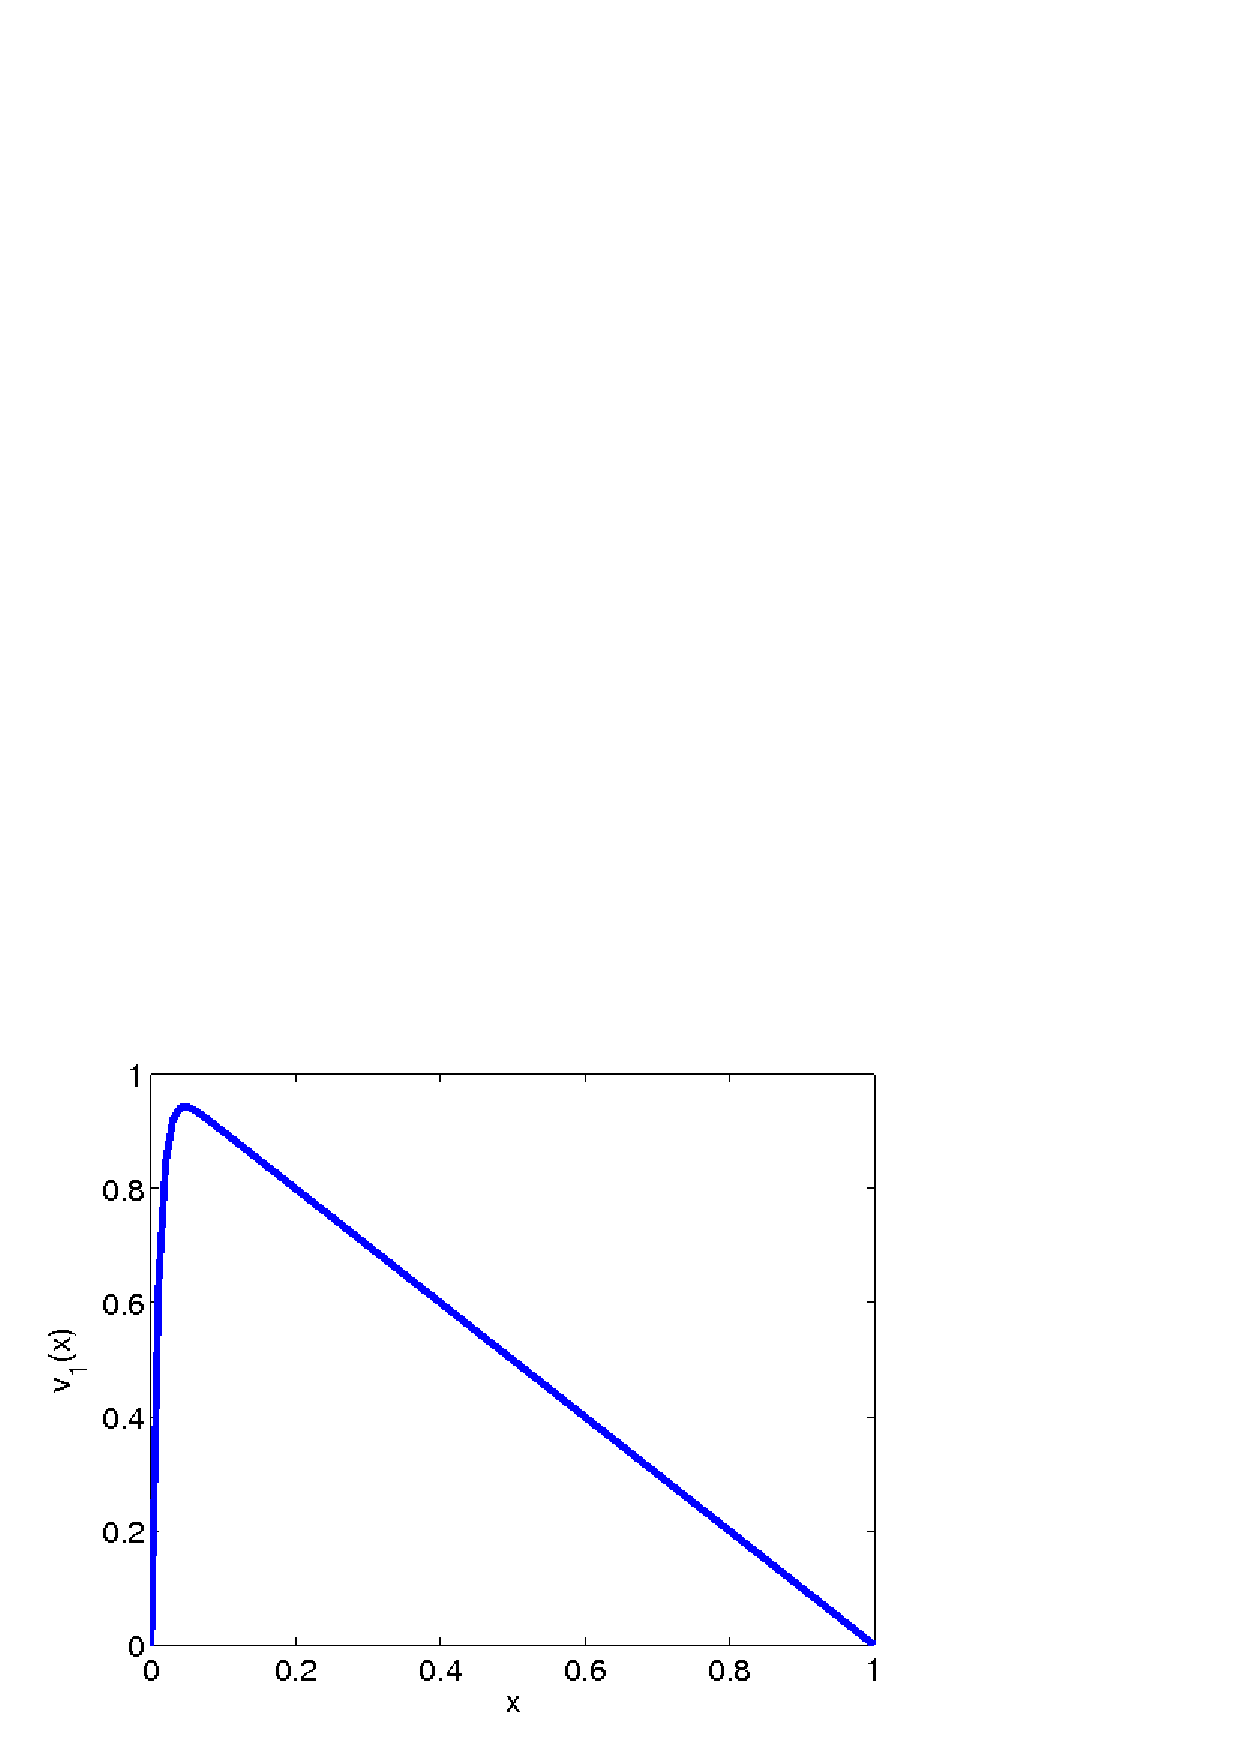
\includegraphics[scale=.5]{figs/testBoundary1D.png}
\caption{$v_1(x) = \frac{e^{-\frac{x}{\epsilon}}}{e^{\frac{1}{\epsilon}}-1}\left(e^{\frac{1}{\epsilon}}\left(e^{\frac{x}{\epsilon}}-1\right) + \left(e^{\frac{1}{\epsilon}}-1\right)e^{\frac{x}{\epsilon}}x\right)$, the solution to the adjoint equation for $f=0$ and constant $\beta$ and load $g$ for $\epsilon = .01$.}
\label{fig:testBoundary1D}
\end{figure}
The solution $v_1$ is plotted in Figure~\ref{fig:testBoundary1D}, where we can see that $v_1(x)$ develops strong boundary layers of width $\epsilon$ near the inflow boundary $x=0$. Consequently, $\frac{\epsilon}{2} v_1'(0)^2 \approx \epsilon^{-1}$. Thus, we cannot conclude $\|\beta v'\| \lesssim \|g\|$ when $g$ is a constant,\footnote{Unlike the case of Dirichlet boundary conditions, the inflow condition on $ \widehat{f}_n = u(0)-\epsilon u'(0)$ induces an adjoint boundary condition $\tau(0)=0$, or equivalently $v'(0) = 0$, removing the non-robust term from the estimate.} and as a consequence cannot conclude that the robust error bound $\|u-u_h\|_{L^2} \lesssim \|(u,\sigma,\widehat{u},\widehat{f}_n)-(u_h,\sigma_h,\widehat{u}_h,\widehat{f}_{n,h})\|_E$ holds for the solution $u_h$.  More detailed 1D error bounds for Dirichlet boundary conditions are provided in \cite{DPG3}, and indicate the same lack of robustness under the test norm used thus far.\footnote{Demkowicz and Heuer proved in \cite{DPGrobustness} that for Dirichlet boundary conditions, robustness as $\epsilon \rightarrow 0$ is achieved by the test norm
\[
\|\left(\tau, v\right)\|_{V,w}^2 = \|v\| + \epsilon \|\grad v\| + \|\beta \cdot \grad v\|_{w+\epsilon} + \| \div \tau\|_{w+\epsilon} + \frac{1}{\epsilon}\|\tau\|_{w+\epsilon}
\]
where $\|\cdot \|_{w+\epsilon}$ is a weighted $L^2$ norm, where the weight $w \in (0,1)$ is required to vanish on $\Gamma_-$ and satisfy $\grad w = O(1)$. The need for this weight is necessary to account for the loss of robustness at the inflow.} 

\begin{figure}[h!]
\centering
\subfigure[Primal problem, Dirichlet inflow BC]{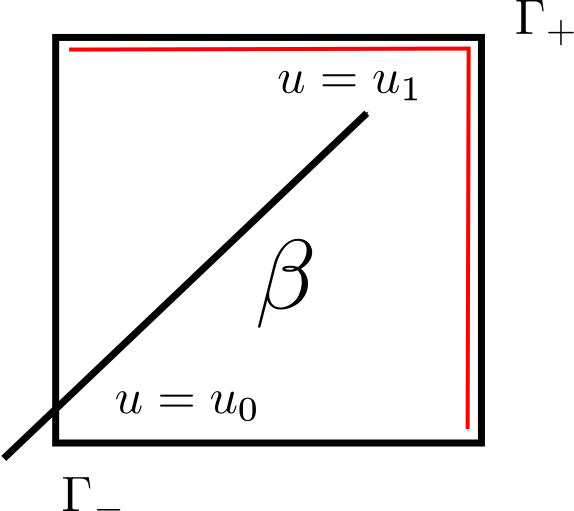
\includegraphics[scale=.3]{figs/primalDir.png}}
\subfigure[Adjoint problem, Dirichlet inflow BC]{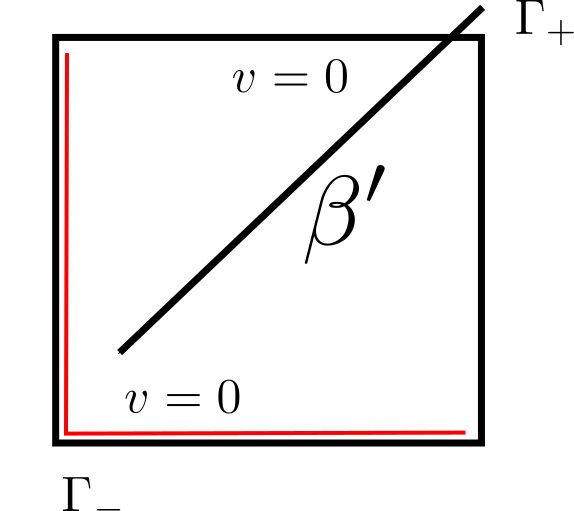
\includegraphics[scale=.3]{figs/adjointDir.png}}
\subfigure[Primal problem, new inflow BC]{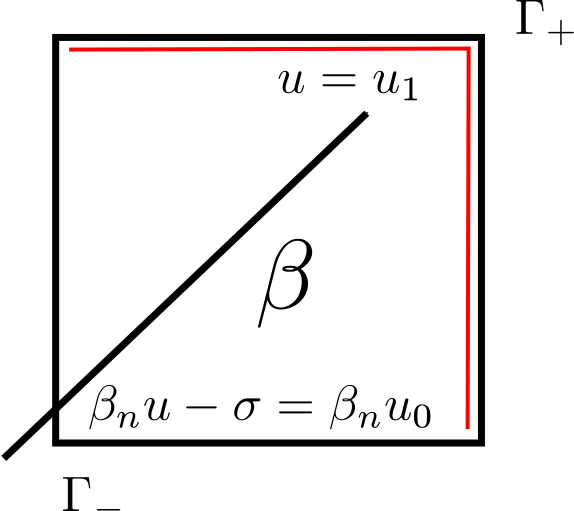
\includegraphics[scale=.3]{figs/primal.png}}
\subfigure[Adjoint problem, new inflow BC]{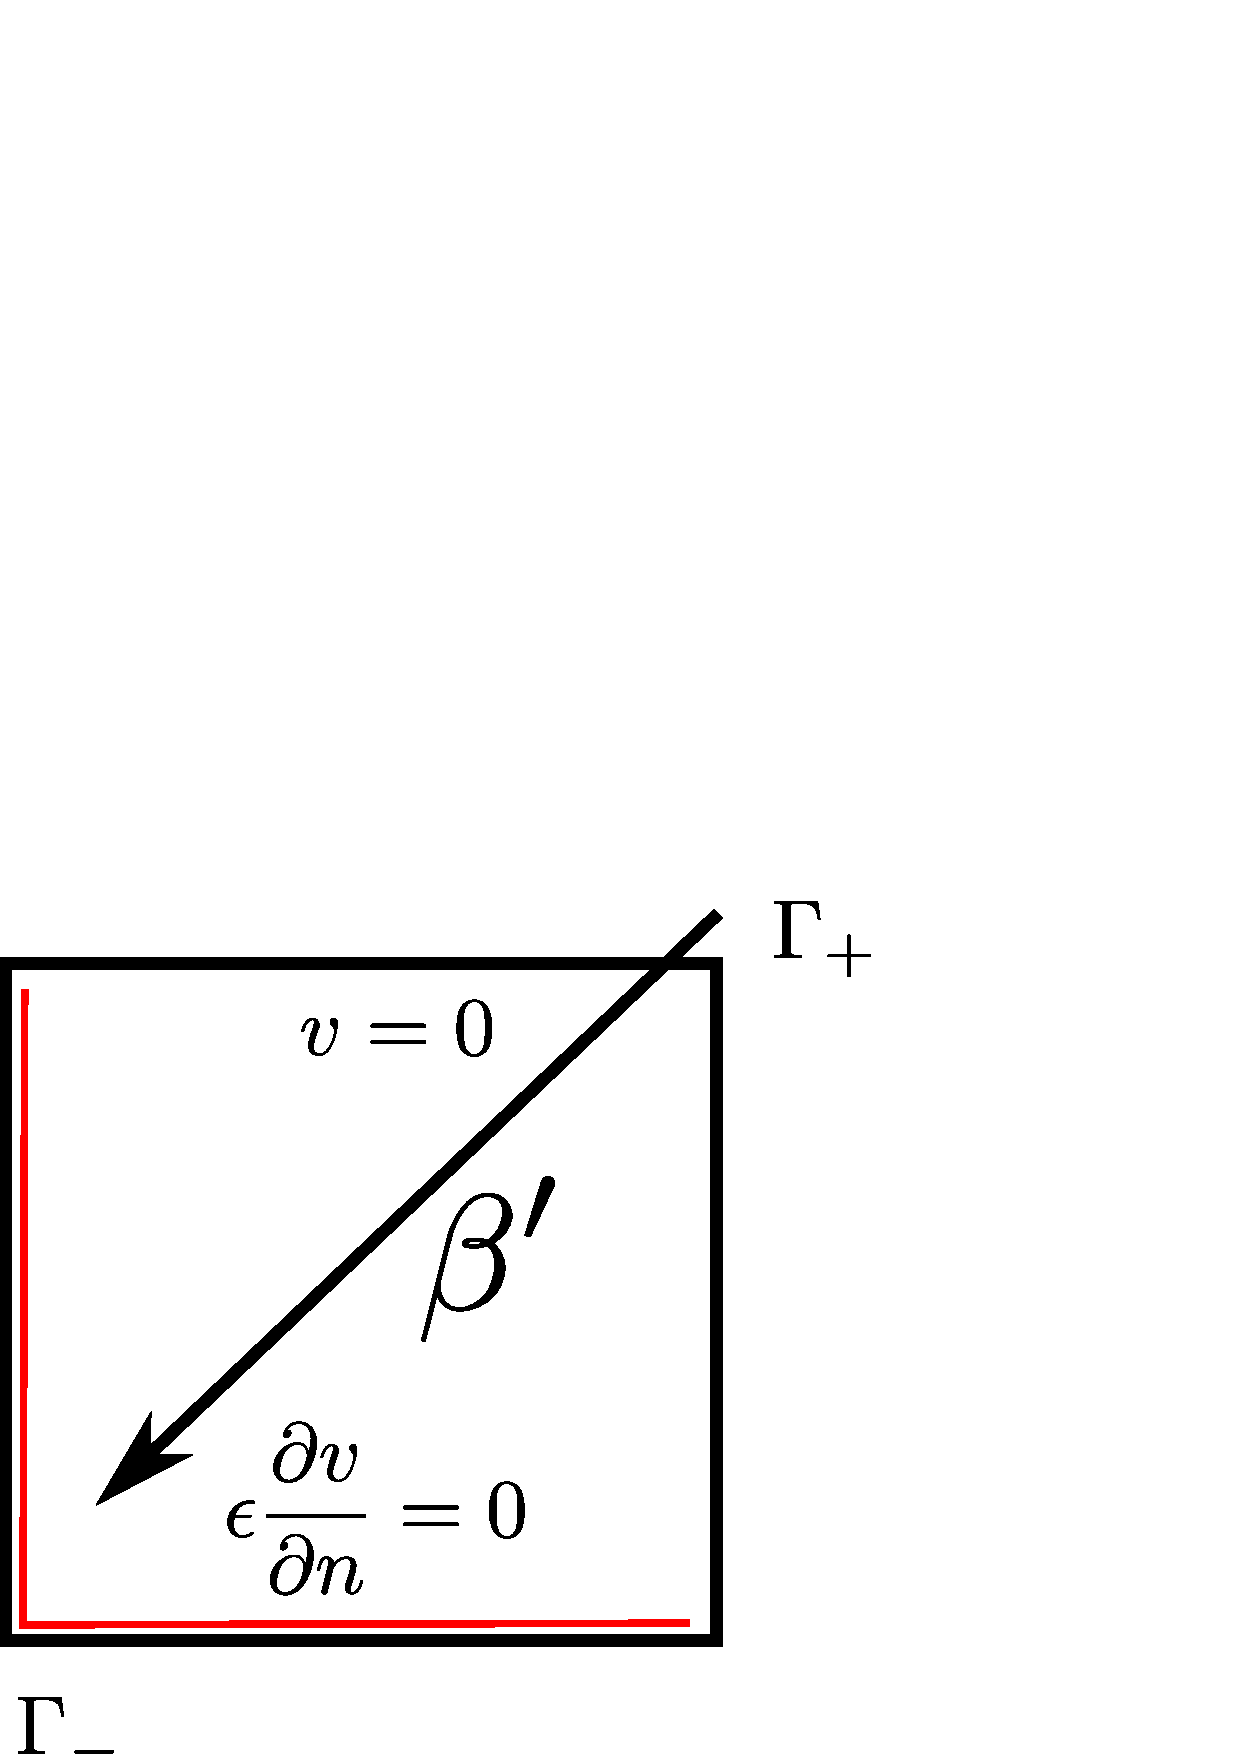
\includegraphics[scale=.3]{figs/adjoint.png}}
\caption{Comparison of primal and adjoint problems under both the standard Dirichlet and the new inflow boundary condition. The outflow boundary for each problem is denoted in red. For the standard Dirichlet inflow condition, the solution to the adjoint problem can develop strong boundary layers at the outflow of the adjoint problem. Notice, under the new inflow conditions, the relaxation of a wall-stop boundary condition with a zero-stress condition at the outflow boundary of the adjoint problem.}
\end{figure}

In higher dimensions, the adjoint problem is of the same form as the primal problem with the direction of convection reversed. However, the primal problem determines adjoint boundary conditions on $\Gamma_-$ and $\Gamma_+$. Thus, wheareas for the primal problem, data is convected from the inflow to the outflow, in the adjoint problem, data is convected from the outflow to the inflow boundary instead. 

We can intuitively explain the loss of robustness under our derived test norm by the presence of the Dirichlet boundary condition on $v$ at the inflow boundary. Since the direction of convection is reversed in the adjoint equation, we can interpret the adjoint as representing the convection of a concentration $v$ from the outflow to the inflow boundary. In the presence of a Dirichlet boundary condition at the inflow, $v$ can develop strong boundary layers at the inflow. As a consequence, the quantities $\|\beta\cdot \grad v\|$ and $\sqrt{\epsilon}\|\grad v\|$ are no longer robustly bounded by $\|f\|$ and $\|g\|$, and we can no longer derive robust bounds on the error $\|u-u_h\|_{L^2}$ by the error in the energy norm.

Recall our strategy for analysis was to decompose of $(v,\tau)$ into continuous and discontinuous portions. Mathematically speaking, the use of Dirichlet boundary conditions on the primal problem introduces strong boundary layers into the solution $v$ of the adjoint equation --- in other words, boundary layers are introduced into the continuous portions of our decomposition of $(v,\tau)$.\footnote{The boundary conditions do not introduce boundary layers into the actual computed test functions. However, an interesting phenomenon observed is that, for small $\epsilon$, a lack of robustness can manifest itself during numerical experiments as additional refinements near the inflow boundary, precisely where the continuous parts of the decomposition of $(v,\tau)$ develop boundary layers.} The new inflow boundary condition on the primal problem relaxes the wall boundary condition induced on the adjoint/dual problem with a boundary condition that does not generate boundary layers, resulting in stronger stability estimates for the adjoint, and a better result for the primal problem. 

%\begin{figure}[h]
%\centering
%\subfigure[Primal problem]{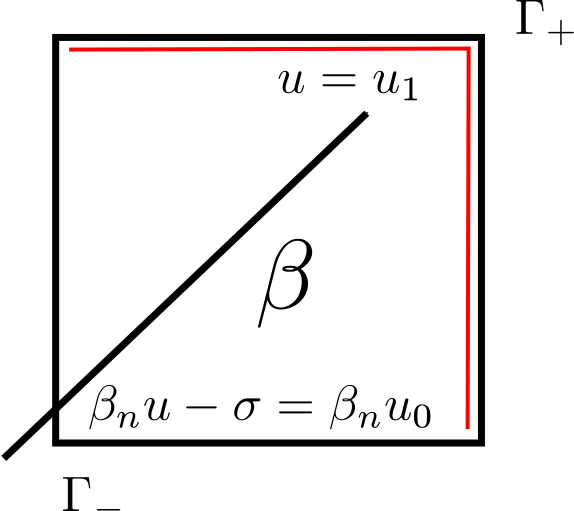
\includegraphics[scale=.3]{figs/primal.png}}
%\subfigure[Adjoint problem]{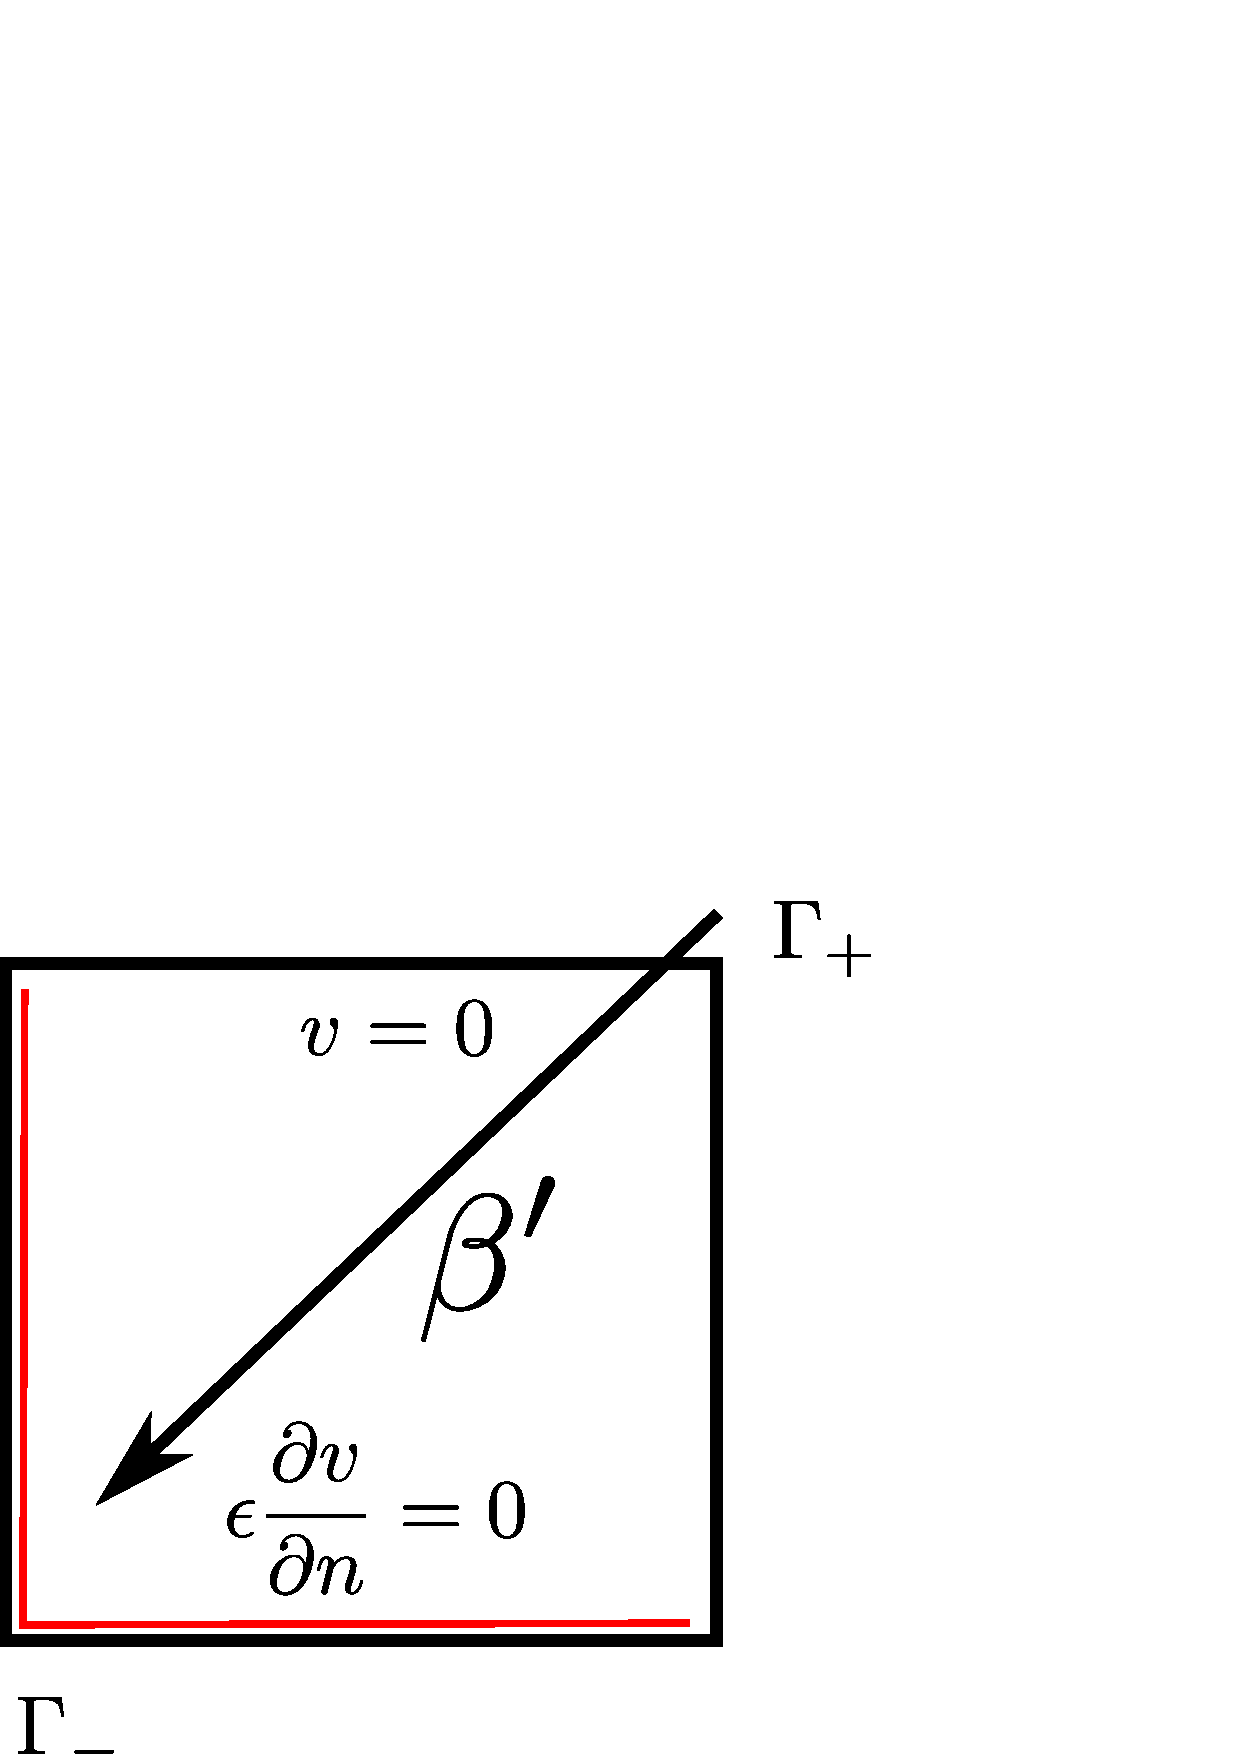
\includegraphics[scale=.3]{figs/adjoint.png}}
%\caption{Comparison of primal and adjoint problems for convection-diffusion under the standard Dirichlet outflow boundary condition and the new inflow boundary condition. Notice the replacement of a wall-stop boundary condition with a Neumann stress boundary condition at the outflow boundary of the adjoint problem. }
%\end{figure}

\section{Numerical experiments}
\label{sec:num_exp}

In each numerical experiment, we vary $\epsilon = .01, .001, .0001$ in order to demonstrate robustness over a range of $\epsilon$.  This is intended to mirror the experience with roundoff effects in numerical experiments \cite{DPGrobustness}; for ``worst-case" linear solvers, such as LU decomposition without pivoting, the effect of roundoff error becomes evident in the solving of optimal test functions for $\epsilon \leq O(1e-5)$.  The roundoff itself comes from the conditioning of the Gram matrix under certain test norms; for example, if the weighted $H({\rm div};\Omega)\times H^1(\Omega)$ norm is used for the test norm $\|\left(\tau,v\right)\|_V$ (as was done in \cite{DPG2}), for an element of size $h$, $\|v\|_{L^2}^2 = O(h)$, while $\|\grad v\|_{L^2}^2 = O(h^{-1})$. As $h\rightarrow 0$, the seminorm portion of the test norm dominates the Gram matrix, leading to a near-singular and ill-conditioned system. 

The effect of roundoff error is often characterized by an increase in the energy error, which (assuming negligible error in the approximation of test functions) is proven to decrease for any series of refined meshes. These roundoff effects are dependent primarily on the mesh, appearing when trying to fully resolve very thin boundary layers by introducing elements of size $\epsilon$ through adaptivity. The effects of roundoff error were successfully treated in \cite{DPG3} by dynamically rescaling the test norms based on element size, a practical remedy not covered yet by the present analysis. 

\subsection{Eriksson-Johnson model problem}

To confirm our theoretical results, we adopt a modification of a problem first proposed by Eriksson and Johnson in \cite{Eriksson1993}. For the choice of $\Omega = (0,1)^2$, $f=0$, and $\beta = (1,0)^T$, the convection diffusion equation reduces to
\[
\pd{u}{x} - \epsilon \left(\pdd{u}{x}+ \pdd{u}{y}\right) = 0,
\]
which has an exact solution by separation of variables, allowing us to analyze convergence of DPG for a wide range of $\epsilon$.  For boundary conditions, we impose $u=0$ on $\Gamma_+$ and $\beta_n u - \sigma_n$ on $\Gamma_-$, which reduces to
\begin{align*}
u-\sigma_x &= u_0-\sigma_{x,0}, \quad x=0,\\
\sigma_y &=  0, \quad y=0,1,\\
u &= 0, \quad x=1.\\
\end{align*}
In this case, our exact solution is the series
\[
u(x,y) = C_0 + \sum_{n=1}^\infty C_n \frac{\exp(r_2(x-1)-\exp(r_1(x-1)))}{r_1\exp(-r2) - r_2\exp(-r1)}\cos(n\pi y),
\]
where
\begin{align*}
r_{1,2} &= \frac{1 \pm \sqrt{1 + 4 \epsilon\lambda_n}}{2 \epsilon},\\
\lambda_n &= n^2\pi^2 \epsilon.
\end{align*}
The constants $C_n$ depend on a given inflow condition $u_0$ at $x=0$ via the formula
\[
C_n = \int_0^1 u_0(y) \cos(n\pi y).
\]

All computations have been done using the adaptive DPG code Camellia, built on the Sandia toolbox Trilinos \cite{Camellia}.

\subsubsection{Solution with $C_1 = 1, C_{n\neq 1} = 0$}

We begin with the solution taken to be the first non-constant term of the above series.  We set the inflow boundary condition to be exactly the value of $u-\sigma_x$ corresponding to the exact solution.  

\begin{figure}[h!]
\centering
\subfigure{
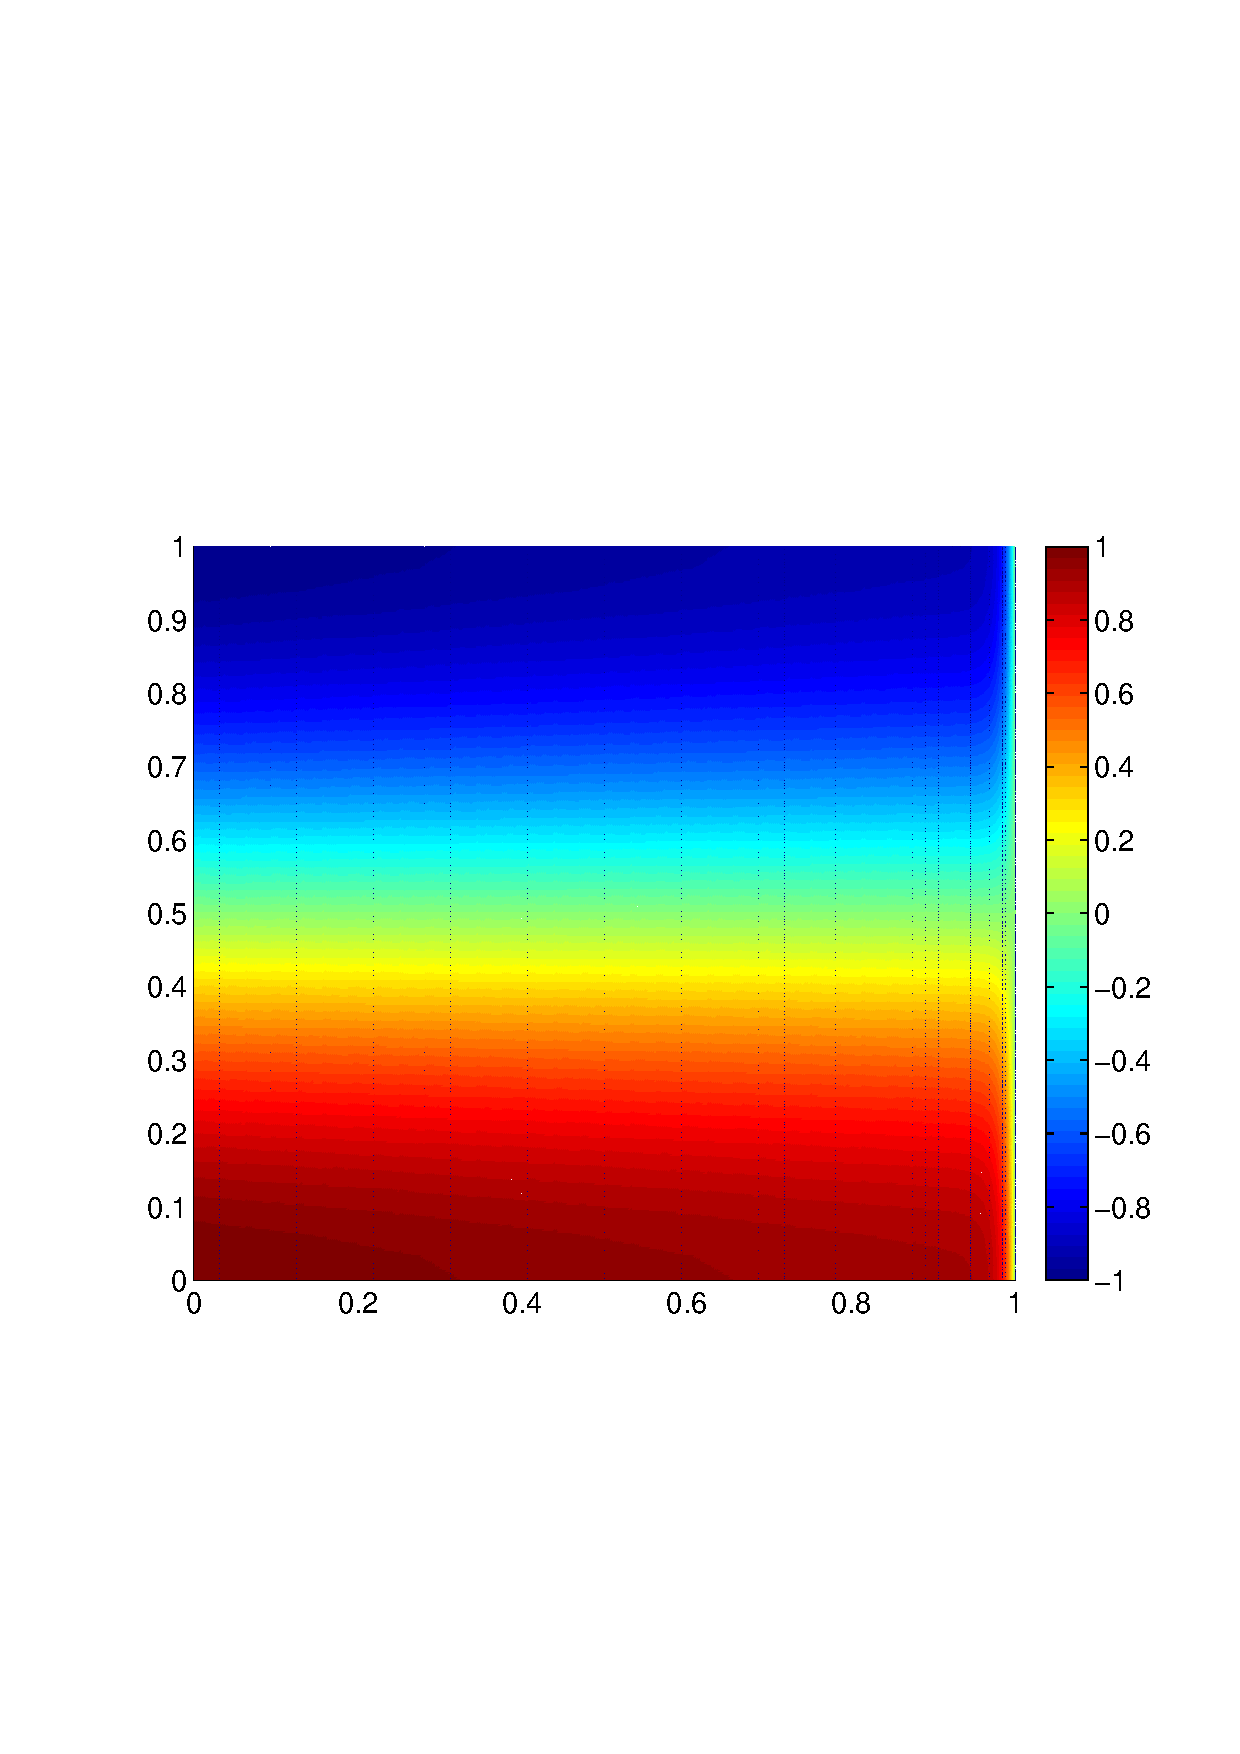
\includegraphics[scale=.37]{figs/wallBC_exact_u.png}
}
\subfigure{
\includegraphics[scale=.37]{figs/wallBC_exact_sigx.png}
}
\subfigure{
\includegraphics[scale=.37]{figs/wallBC_exact_sigy.png}
}
\caption{Solution for $u$, $\sigma_x$, and $\sigma_y$ for $\epsilon = .01$, $C_1 = 1$, $C_n=0$, $n\neq 1$}
\end{figure}
In each case, we begin with a square 4 by 4 mesh of quadrilateral elements with order $p=3$.  We choose $\Delta p = 5$, though we note that the behavior of DPG is nearly identical for any $\Delta p \leq 3$, and qualitatively the same for $\Delta p = 2$.  $h$-refinements are executed using a greedy refinement algorithm, where element energy error $e_K^2$ is computed for all elements $K$, and elements such that $e_K^2 \leq \alpha \max_K e_K^2$ are refined.  We make the arbitrary choice of taking $\alpha = .2$ for each of these experiments.  

\begin{figure}[h!]
\centering
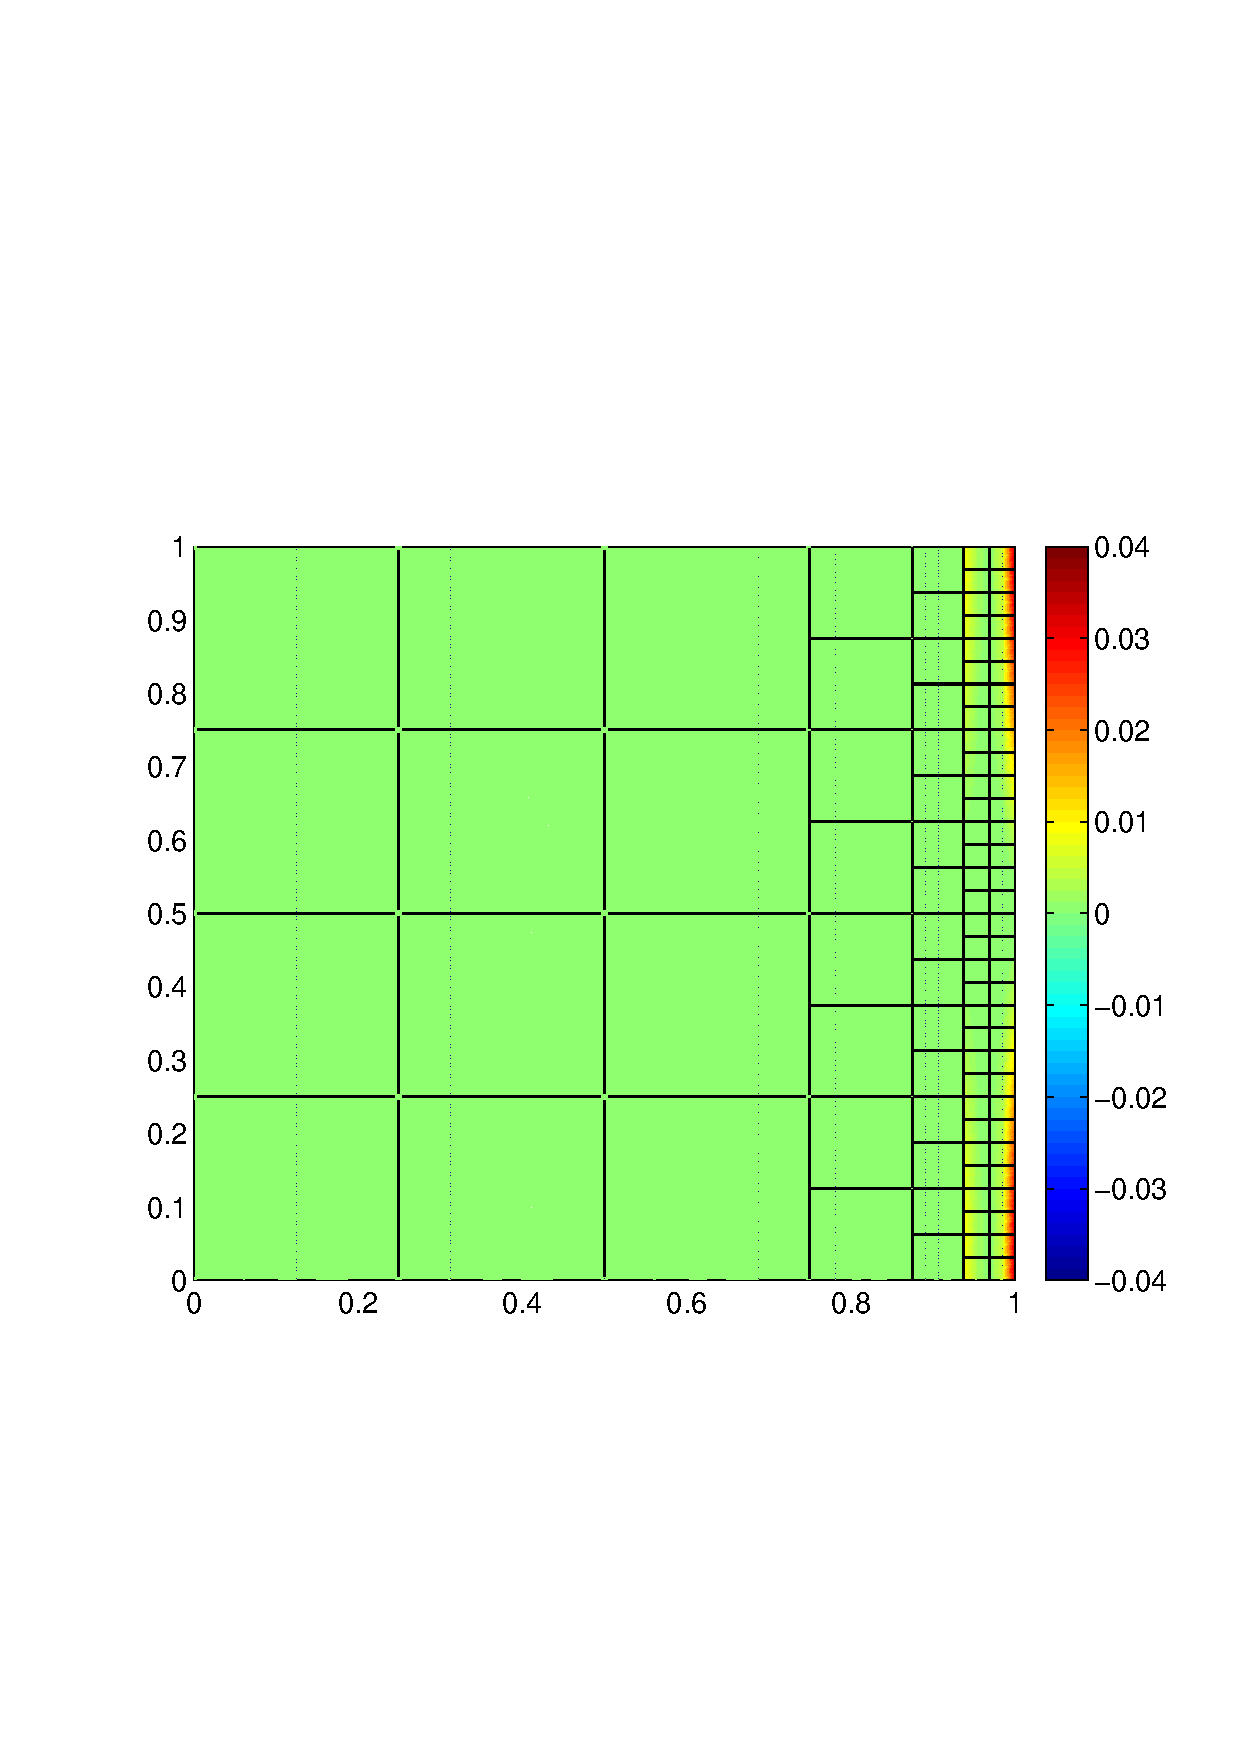
\includegraphics[scale=.4]{figs/u_pointdiff_wallBC.png}
\caption{Adapted mesh and pointwise error for $\epsilon=.01$}
\end{figure}
We are especially interested in the ratio of energy error and total $L^2$ error in both $\sigma$ and $u$, which we denote as $\|u-u_h\|_{L^2}$.  The bounds on $\nor{\cdot}_E$ presented in Section~\ref{sec:main_bounds} imply that, using the above test norm, $\|u-u_h\|_{L^2} / \|u-u_h\|_E \leq C$ independent of $\epsilon$.  Figure~\ref{ratios_simple}, which plots the ratio of $L^2$ to energy error, seems to imply that (at least for this model problem) $C=O(1)$.  Additionally, while we do not have a robust lower bound ($\|u-u_h\|_{L^2} / \|u-u_h\|_E$ can approach $0$ as $\epsilon \rightarrow 0$), our numerical results appear to indicate the existence of an $\epsilon$-independent lower bound. 

\begin{figure}[h!]
\centering
\subfigure{
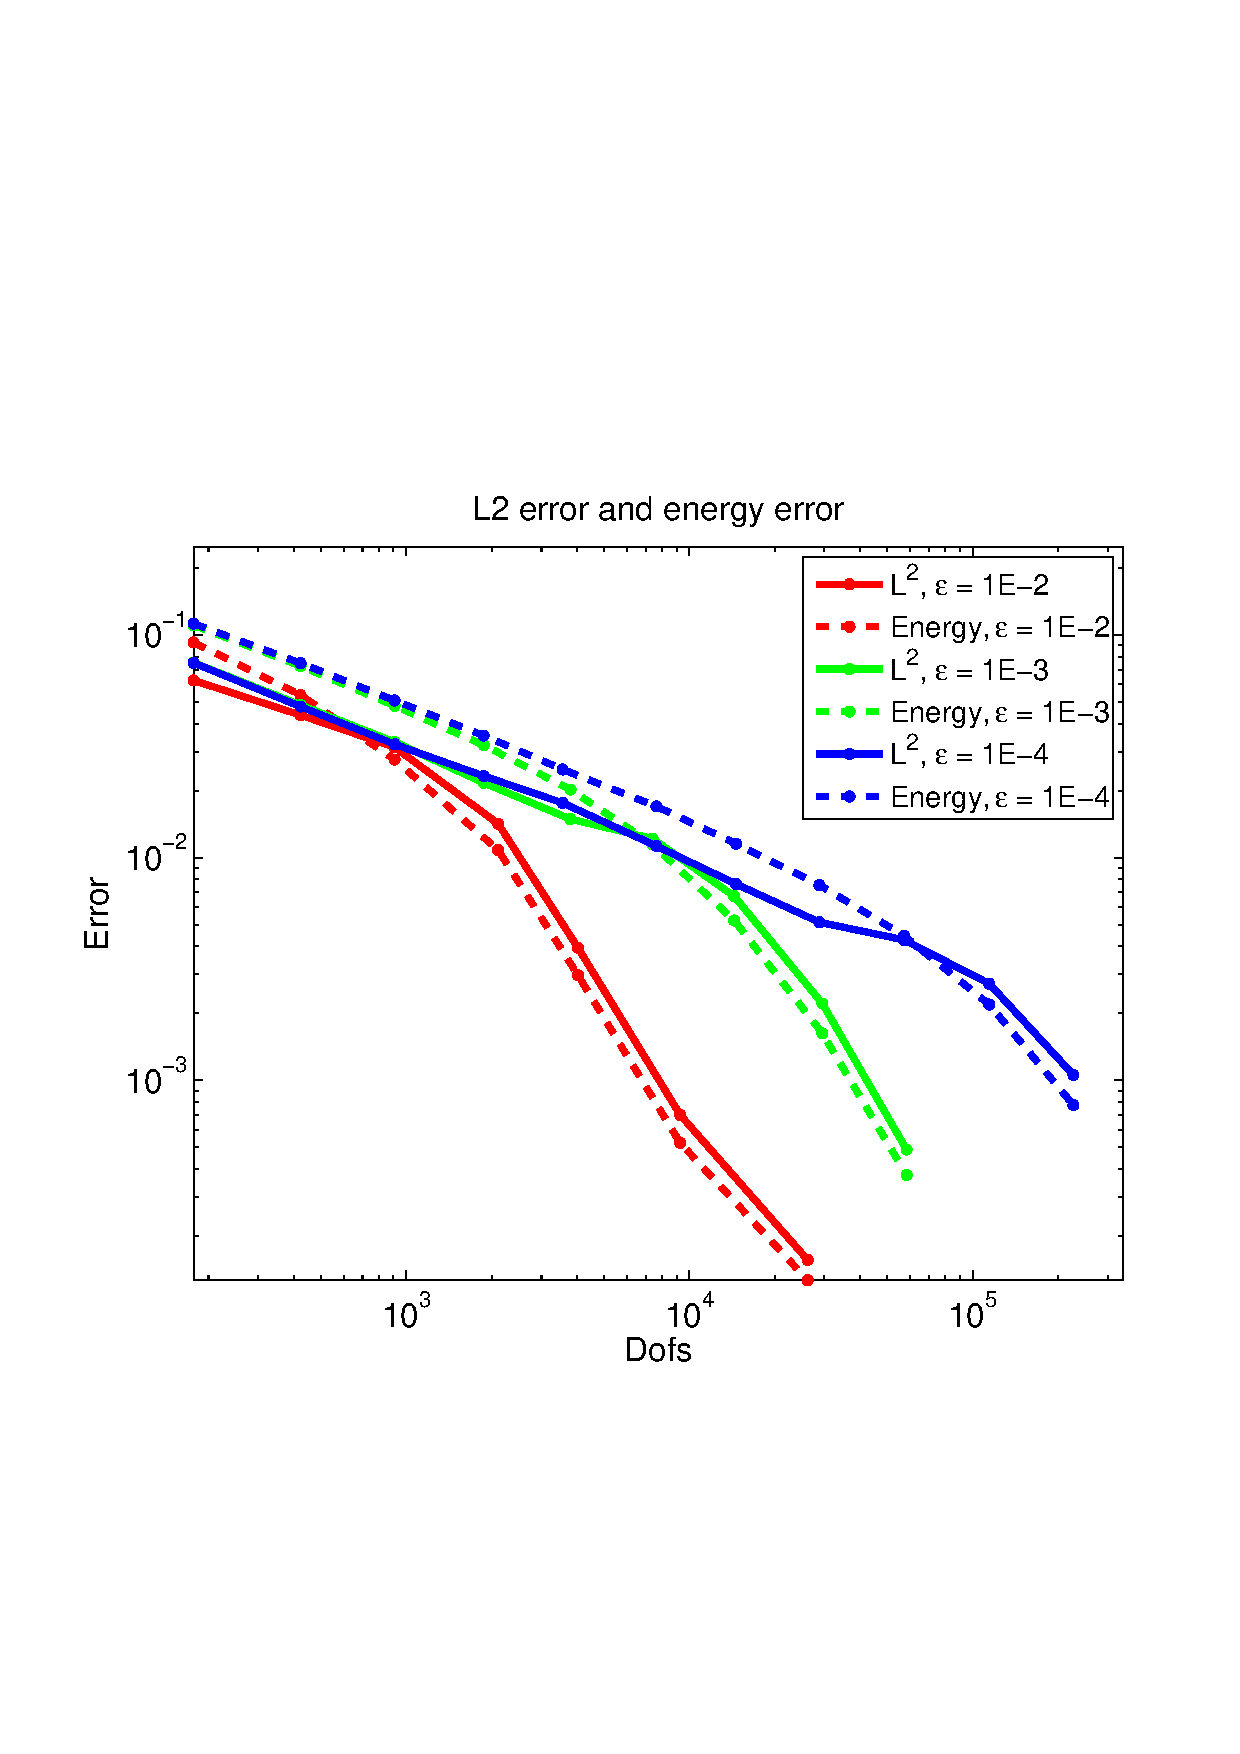
\includegraphics[scale=.38]{figs/errorrates_wallBC.png}
}
\subfigure{
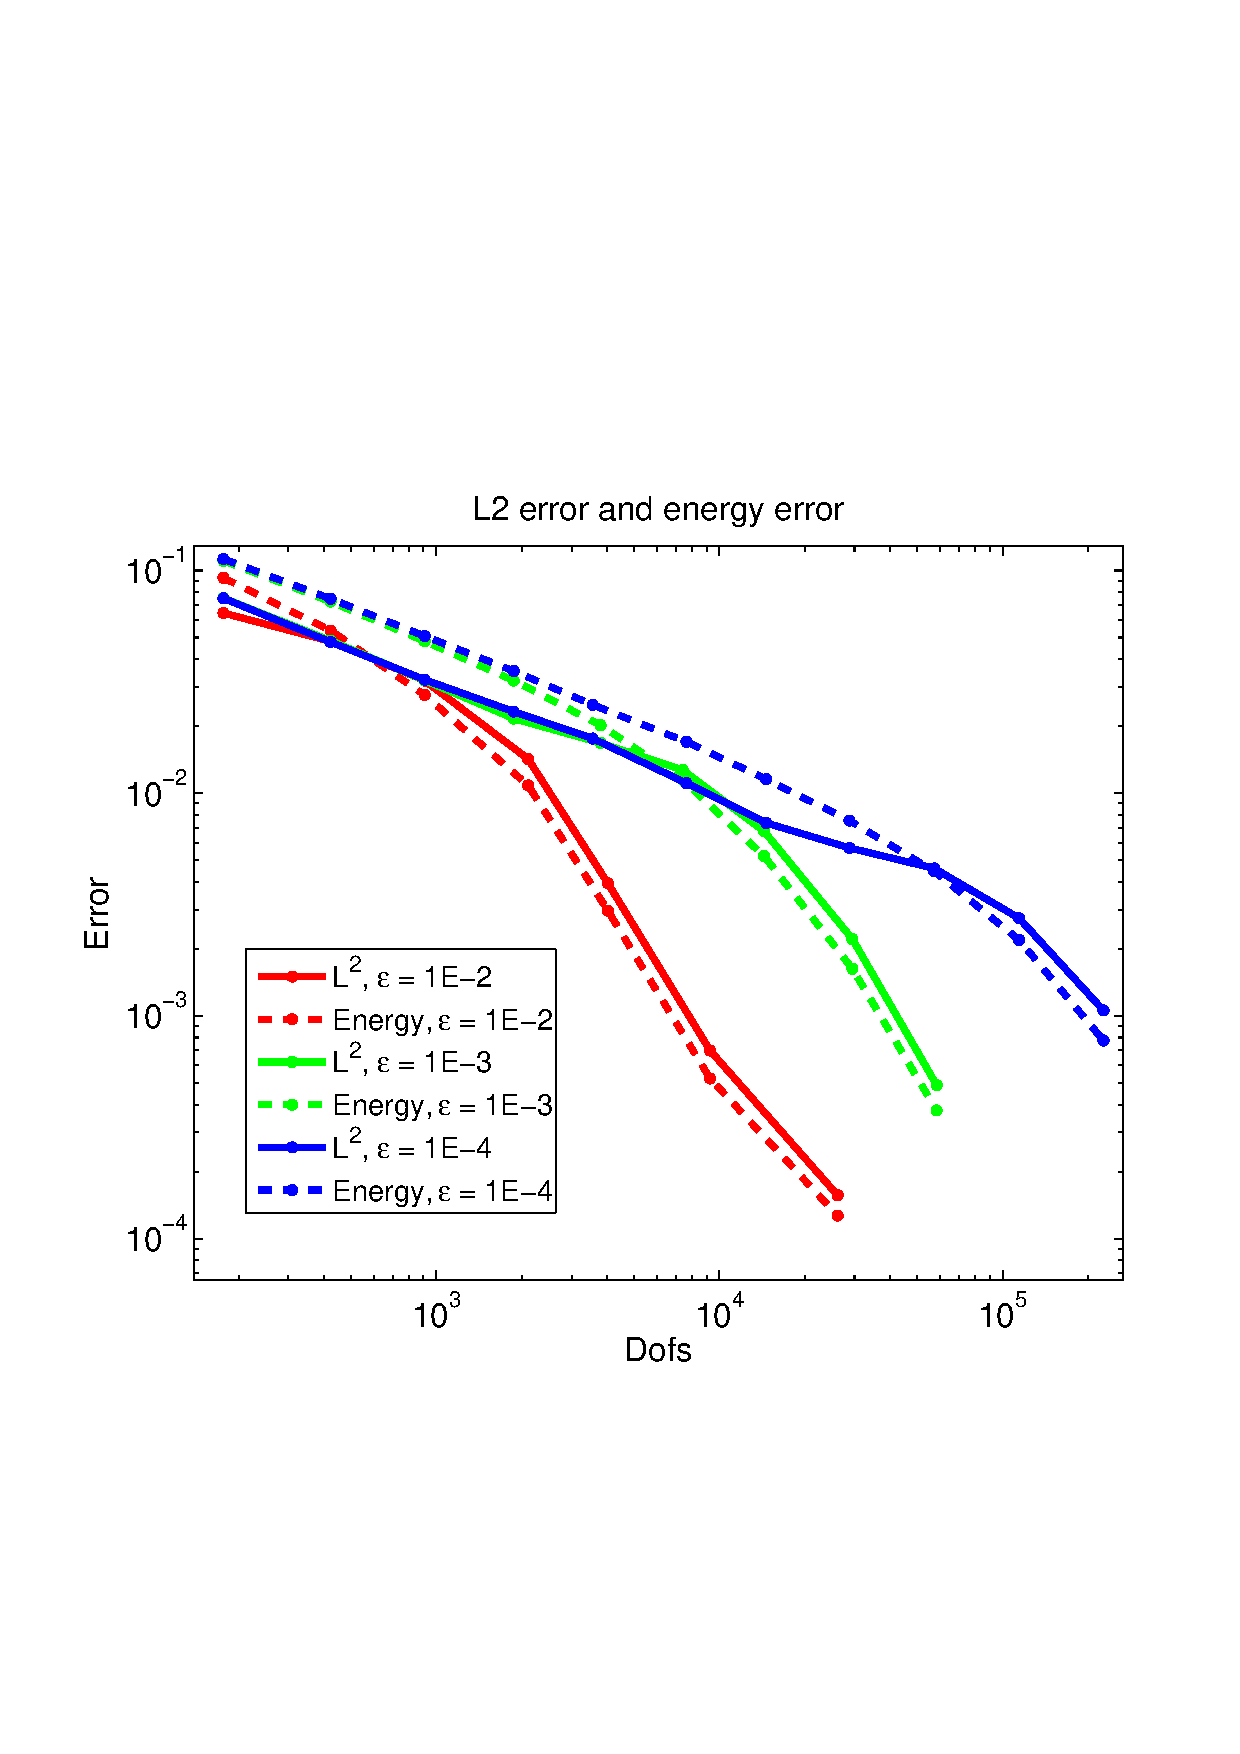
\includegraphics[scale=.38]{figs/L2energyratio_wallBC.png}
}
\caption{$L^2$ and energy errors, and their ratio for $\epsilon=.01$, $\epsilon=.001$, $\epsilon=.0001$}
\label{ratios_simple}
\end{figure}
The effect of a mesh dependent scalings on the $\|v\|^2$ and $\|\tau\|^2$ terms in the test norm can be seen in the ratios of $L^2$ to energy error; as the mesh is refined, the constants in front of the $L^2$ terms for $v$ and $\tau$ converge to stationary values (providing the full robustness implied by our adjoint energy estimates), and the ratio of $L^2$ to energy error transitions from a smaller to a larger value.  The transition point happens later for smaller $\epsilon$, which we expect, since the transition of the ratio corresponds to the introduction of elements whose size is of order $\epsilon$ through mesh refinement. 

We examined how small $\epsilon$ needed to be in order to encounter roundoff effects as well. In \cite{DPGrobustness}, the smallest resolvable $\epsilon$ using only double precision arithmetic was $1e-4$. The solution of optimal test functions is now done using both pivoting and equilibration, improving conditioning. Roundoff effects still appear, but at smaller values of $\epsilon$.

\begin{figure}[h!]
\centering
\subfigure{
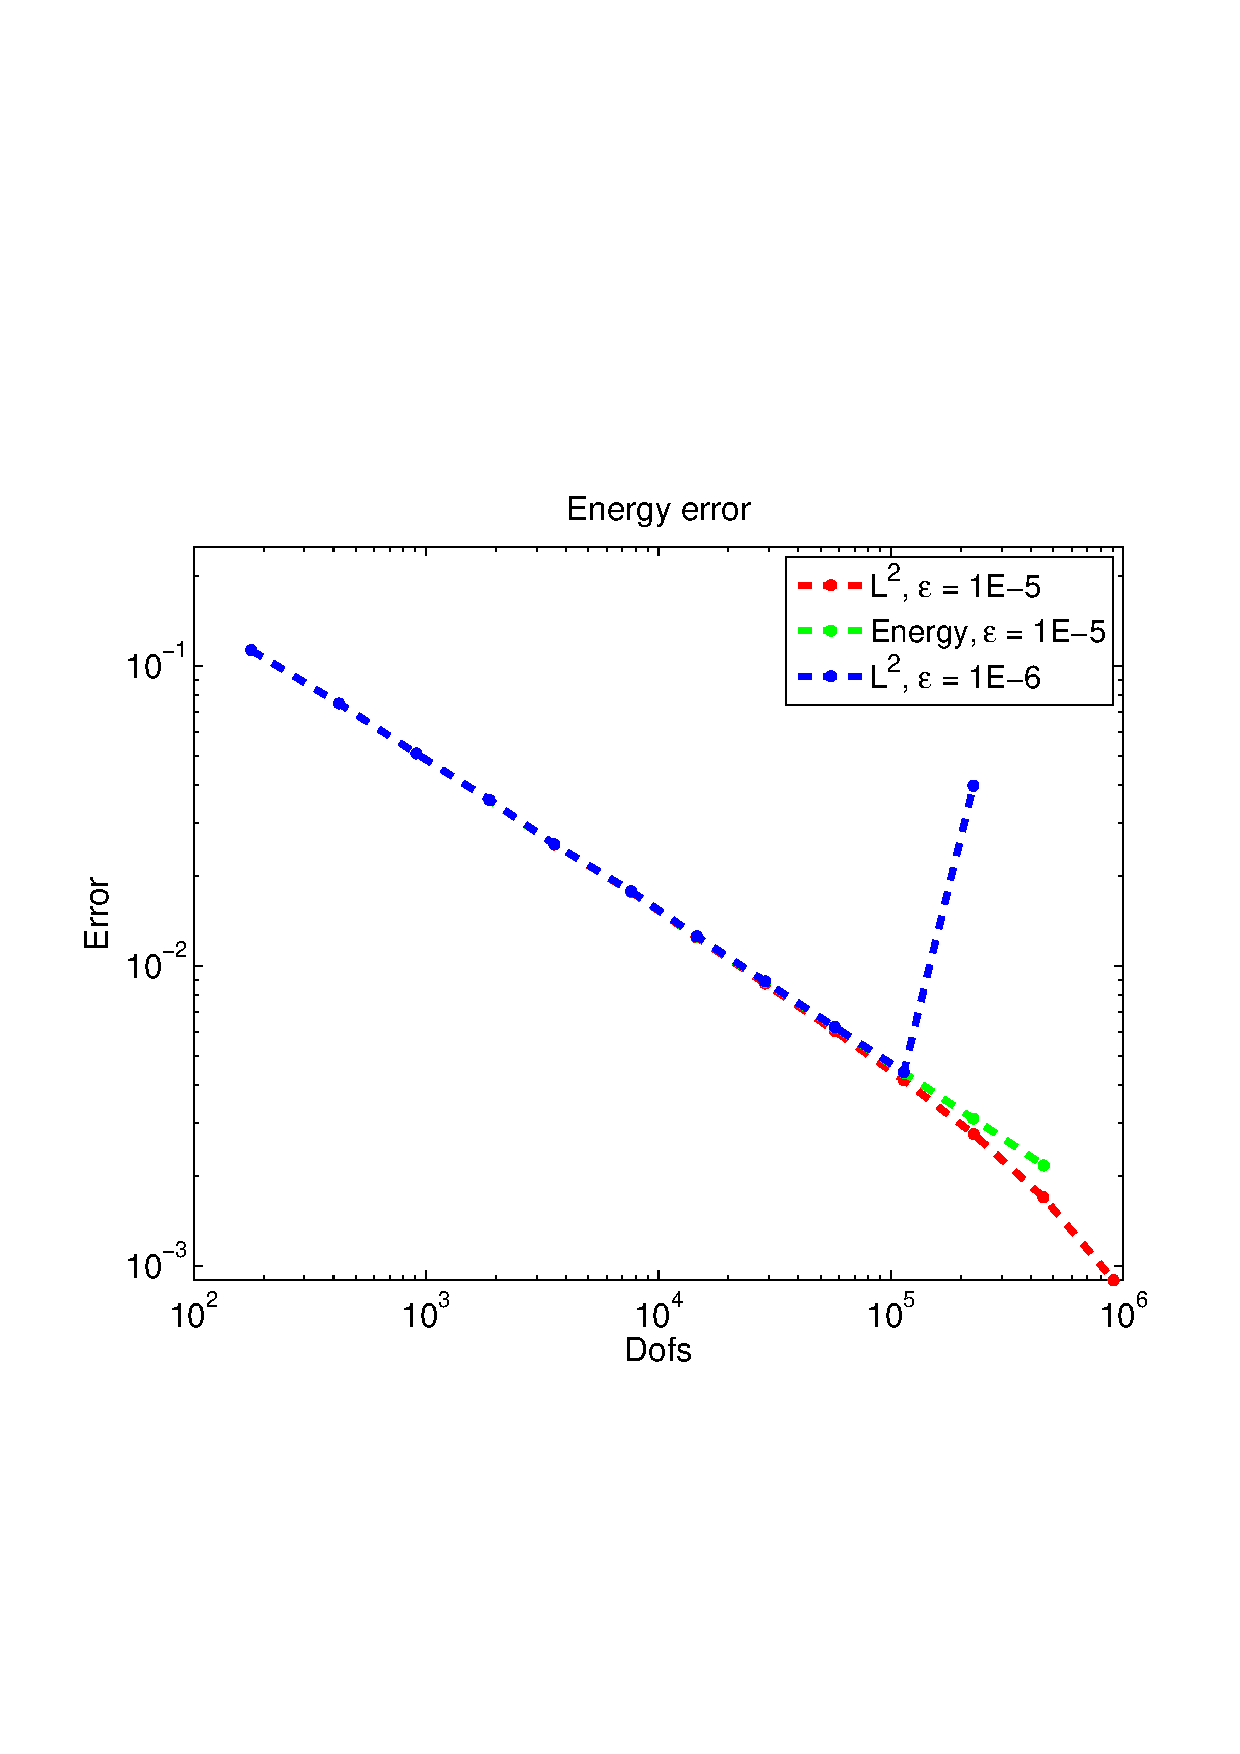
\includegraphics[scale=.36]{figs/roundoff_rates.png}
}
\subfigure{
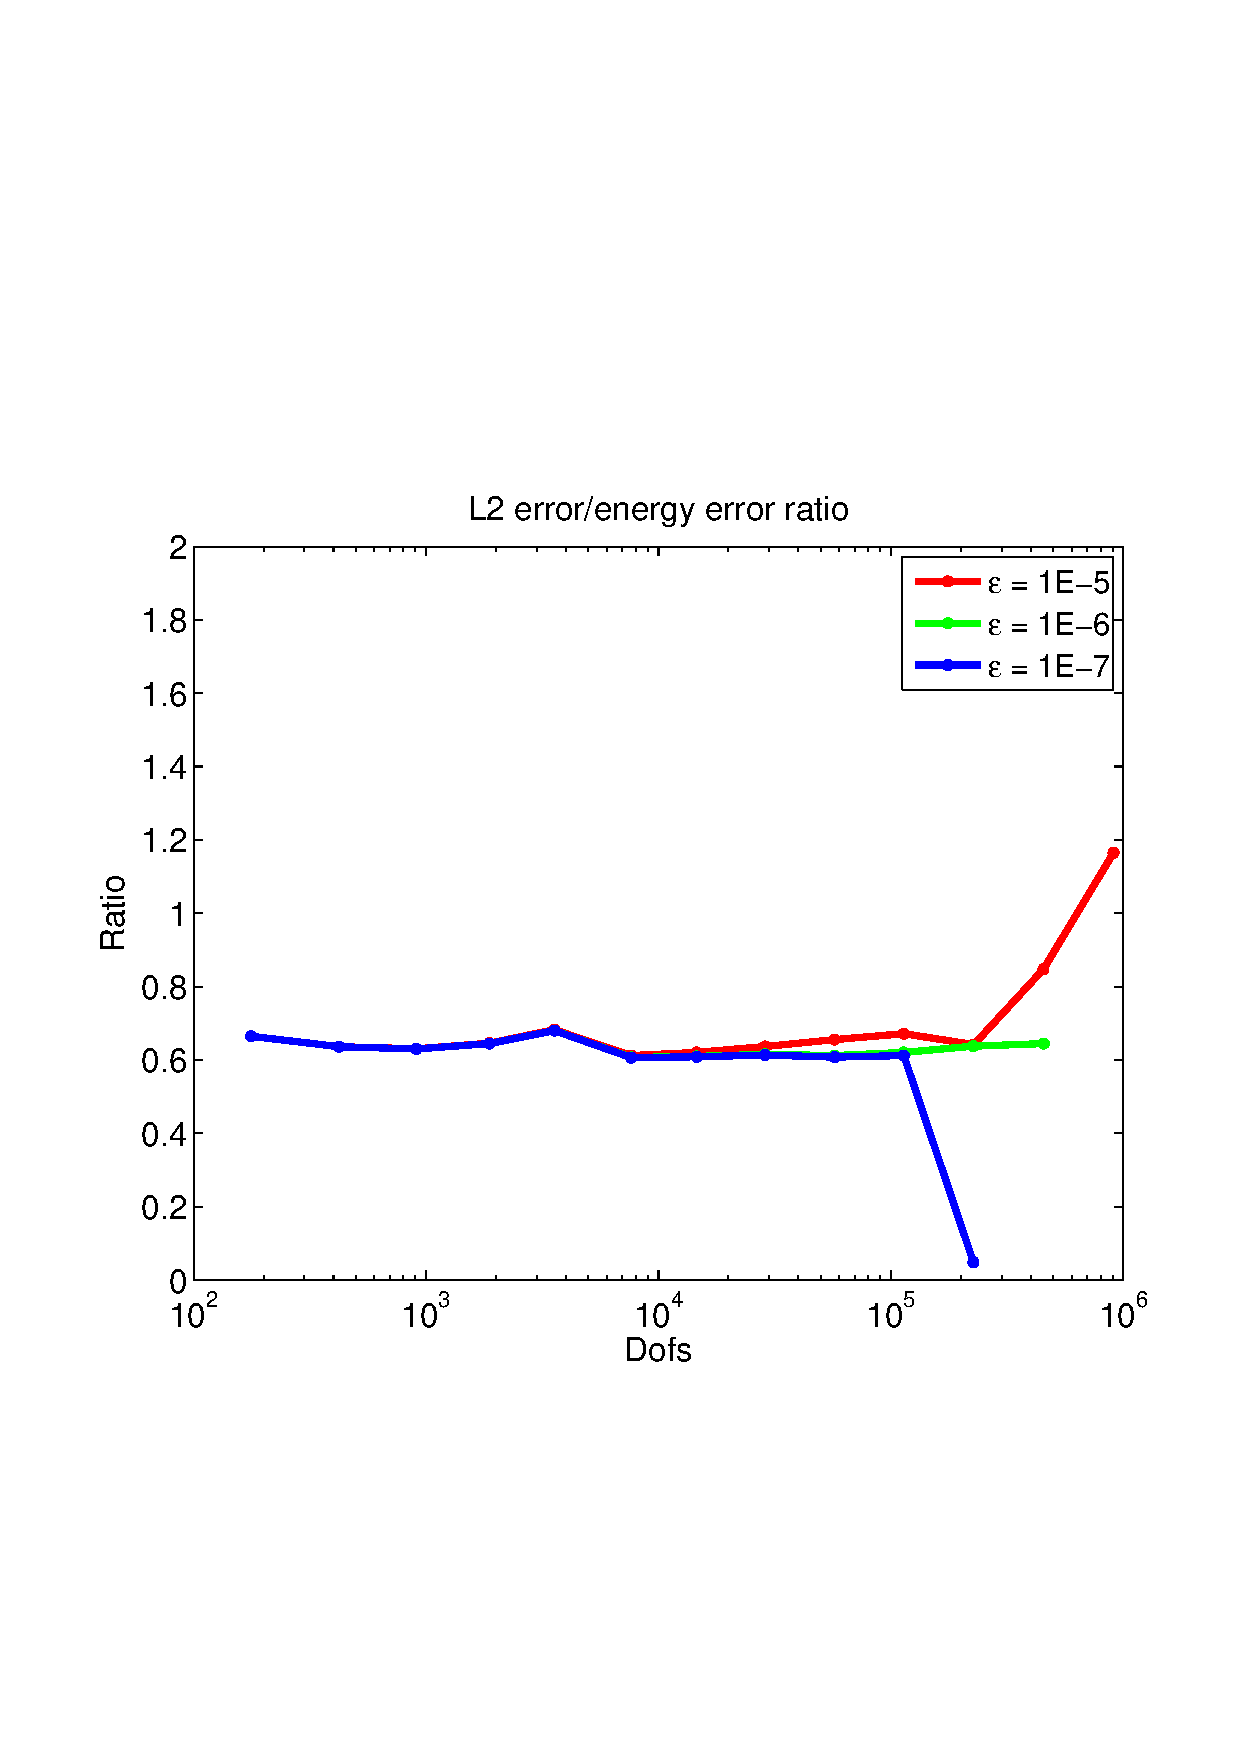
\includegraphics[scale=.36]{figs/roundoff_ratio.png}
}
\caption{Energy error and $L^2$/energy error ratio for $\epsilon=1e-5$, $\epsilon=1e-6$, $\epsilon=1e-7$. Non-monotonic behavior of the energy error indicates conditioning issues and roundoff effects.}
\label{roundoff_figures}
\end{figure}

Without anisotropic refinements, it still becomes computationally difficult to fully resolve the solution for $\epsilon$ smaller than $1e-5$. Regardless, for all ranges of $\epsilon$, DPG does not lose robustness, as indicated by the rates and ratio between $L^2$ and energy error in Figure~\ref{roundoff_figures} remaining bounded from both above and below. For $\epsilon = 1e-5$, we observe that the ratio of $L^2$ error increases, corresponding to the scaling of the test norm with mesh size (the transition in test norm occurs after 8 refinements, which, for an initial $4\times 4$ mesh, implies a minimum element size of about $1.5e-05$. At this point, rescaled test norm allows us to take advantage of the full magnitude of the $L^2$ term for $\|v\|$ and $\|\tau\|$ implied by our adjoint estimates). By analogy, for smaller $\epsilon = 1e-6, 1e-7$, the transition period should begin near the 10th and 11th refinement iterations; however, we do not observe such behavior, possibly due to roundoff effects. 
For $\epsilon=1e-6$, the ratio simply remains constant, but for $\epsilon=1e-7$, we observe definite roundoff effects, as the energy error increases at the 11th refinement. Since DPG is optimal in the energy norm for a mesh-independent test norm\footnote{While the test norm changes with the mesh, it increases monotonically. A strictly stronger test norm implies $\frac{b(u,v)}{\|v\|_1} \geq \frac{b(u,v)}{\|v\|_2}$ for any $\|v\|_1 \leq \|v\|_2$}, we expect monotonic decrease of the energy error with mesh refinement. Non-monotonic behavior indicates either approximation or roundoff error, and as we observed no qualitative difference between using $\Delta p = 5$ and $\Delta p = 6$ for these experiments, we expect that the approximation error is negligible and conclude roundoff effects are at play when these phenomena are observed. 

It is worth noting that for $\epsilon \leq 1e-5$, we do not perform enough refinements to completely resolve the boundary layer, so $|K| \geq \epsilon$ for all $K\in \Oh$. Thus, any roundoff effects observed are not due to the conditioning issues associated with the differing scales of the $\nor{v}_{L^2(K)}$ and $\nor{\grad v}_{L^2(K)}$ terms discussed previously. 

\subsubsection{Neglecting $\sigma_n$}

In practice, we will not have prior knowledge of $\sigma_n$ at the inflow, and will have to set $\beta_n u - \sigma_n = u_0$, ignoring the viscous contribution to the boundary condition.  The hope is that for small $\epsilon$, this omission will be negligible. Figure~\ref{ratios_noSigma} indicates that, between $\epsilon = .005$ and $\epsilon = .001$, the omission of $\sigma_n$ in the boundary condition becomes negligible, and both our error rates and ratios of $L^2$ to energy error become identical to the case where $\sigma_n$ is explicitly accounted for in the inflow condition. For large $\epsilon = .01$, the $L^2$ error stagnates around $1e-3$, or about $7\%$ relative error. 

\begin{figure}[h!]
\centering
\subfigure{
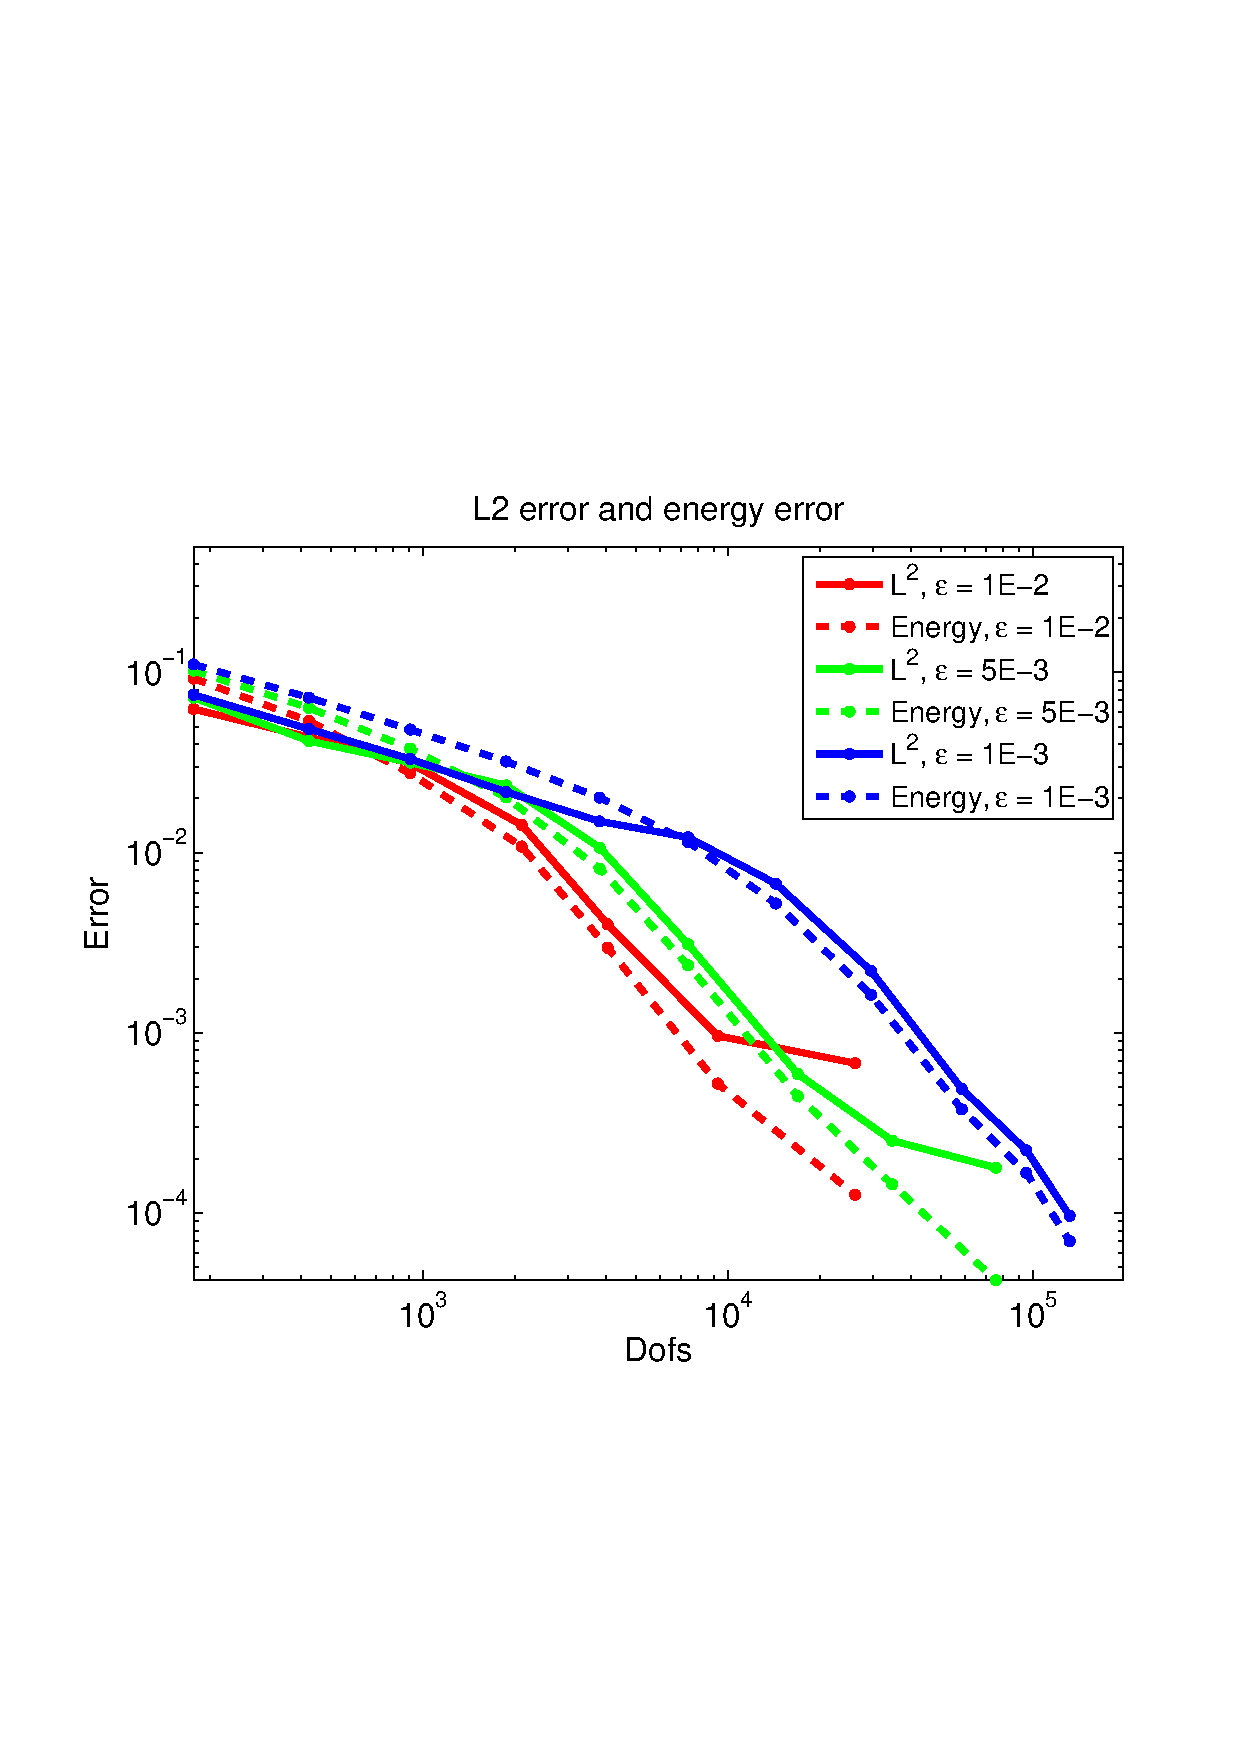
\includegraphics[scale=.38]{figs/rates_noSigma.png}
}
\subfigure{
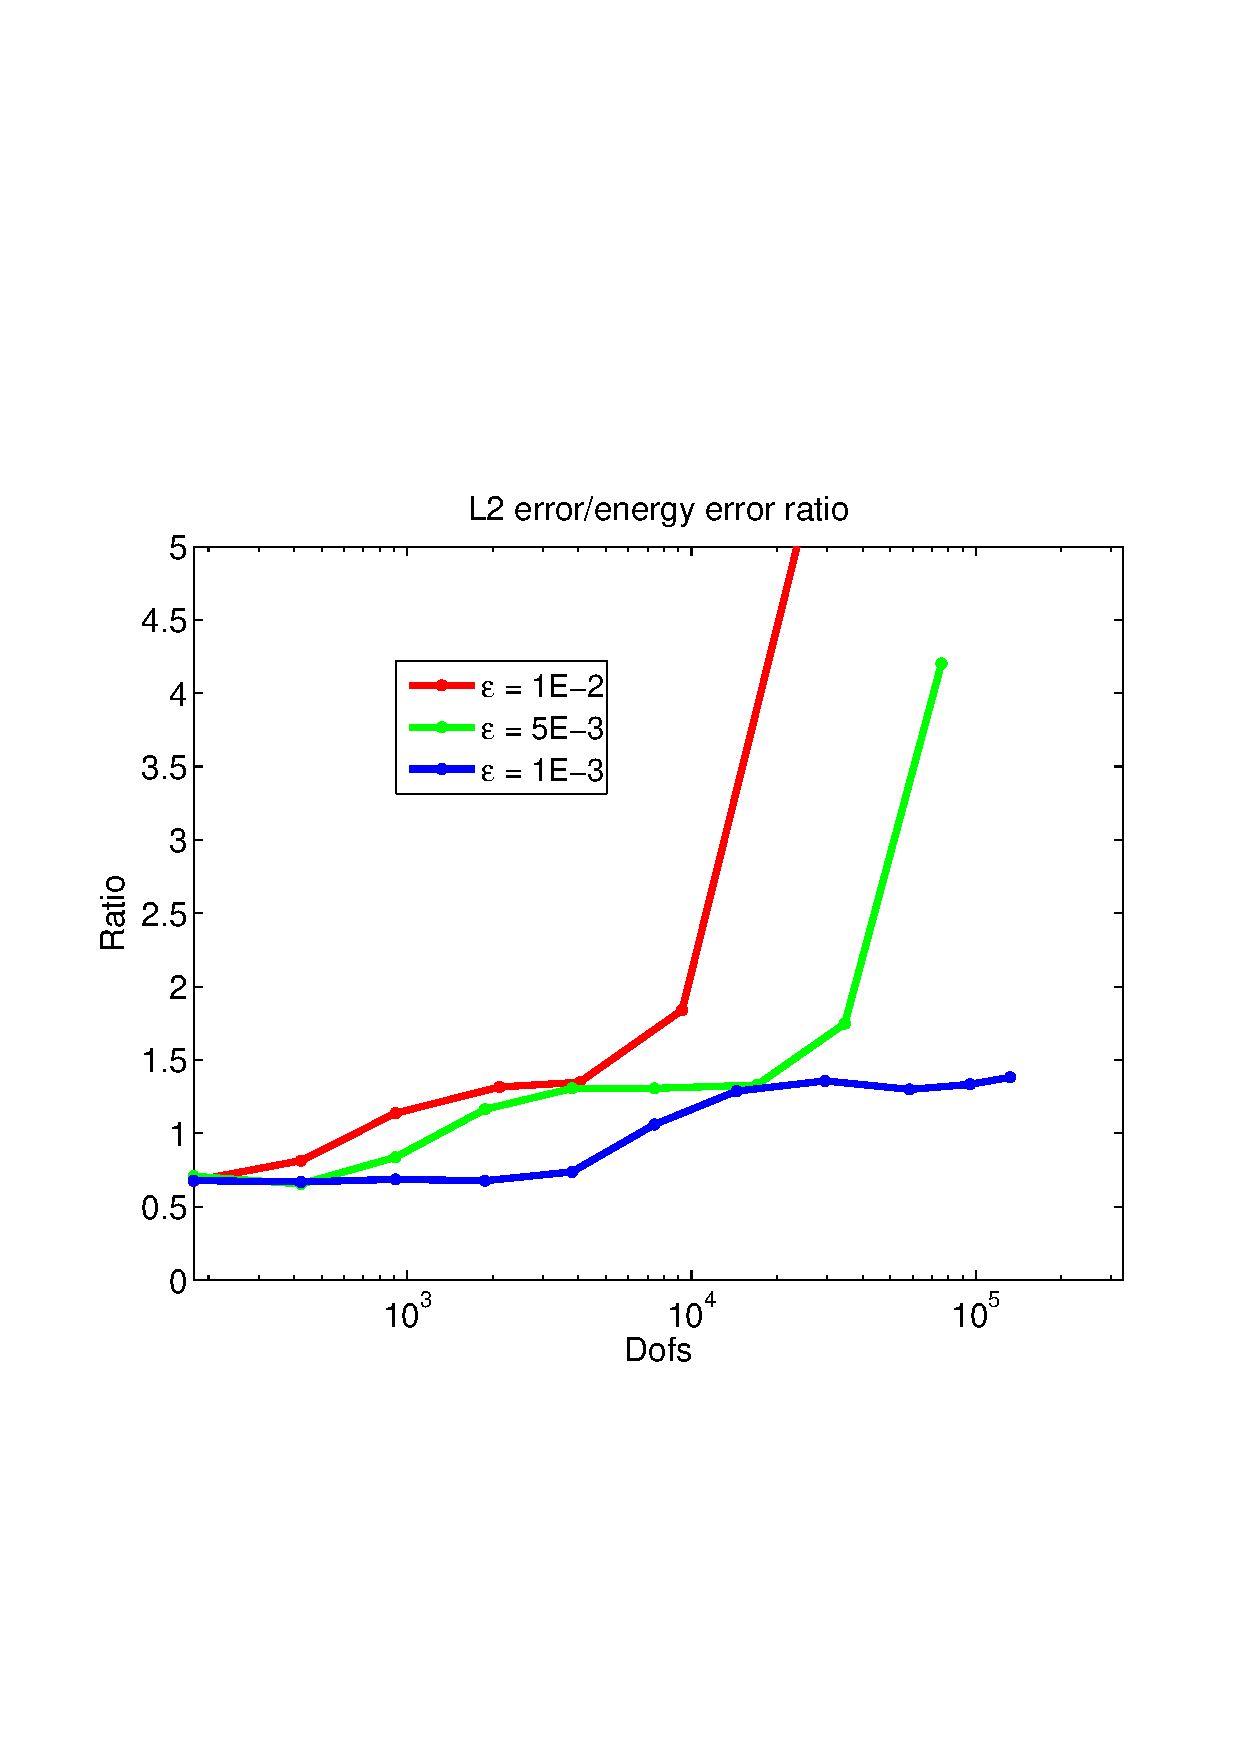
\includegraphics[scale=.38]{figs/ratio_noSigma.png}
}
\caption{$L^2$ and energy errors and their ratio when neglecting $\sigma_n$ at the inflow.}
\label{ratios_noSigma}
\end{figure}

\subsubsection{Discontinuous inflow data}

We note also that an additional advantage of selecting this new boundary condition is a relaxation of regularity requirements: as $\widehat{f}_n \in H^{-1/2}(\Gh)$, strictly discontinuous inflow boundary conditions are no longer ``variational crimes".  We consider the discontinuous inflow condition
\[
u_0(y) = \begin{cases}
(y-1)^2, \quad &y>.5\\
-y^2, \quad &y\leq .5 
\end{cases}
\]
as an example of a more difficult test case. 

\begin{figure}[h!]
\centering
\subfigure{
\includegraphics[scale=.38]{figs/disc_hat.png}
}
\subfigure{
\includegraphics[scale=.38]{figs/disc_hat_surf.png}
}
\caption{Solution variables $u$ and $\widehat{u}$ with discontinuous inflow data $u_0$ for $\epsilon = .01$.}
\label{disc_sol}
\end{figure}
Figure~\ref{disc_sol} shows the solution $u$ and overlaid trace variable $\widehat{u}$, which both demonstrate the regularizing effect of viscosity on the discontinuous boundary condition at $x=0$. However, we do not have a closed-form solution with which to compare results for a stricly discontinuous $u_0$.  In order to analyze convergence, we approximate $u_0$ with 20 terms of a Fourier series, giving a near-discontinuity for $u_0$.  

\begin{figure}[h!]
\centering
\subfigure{
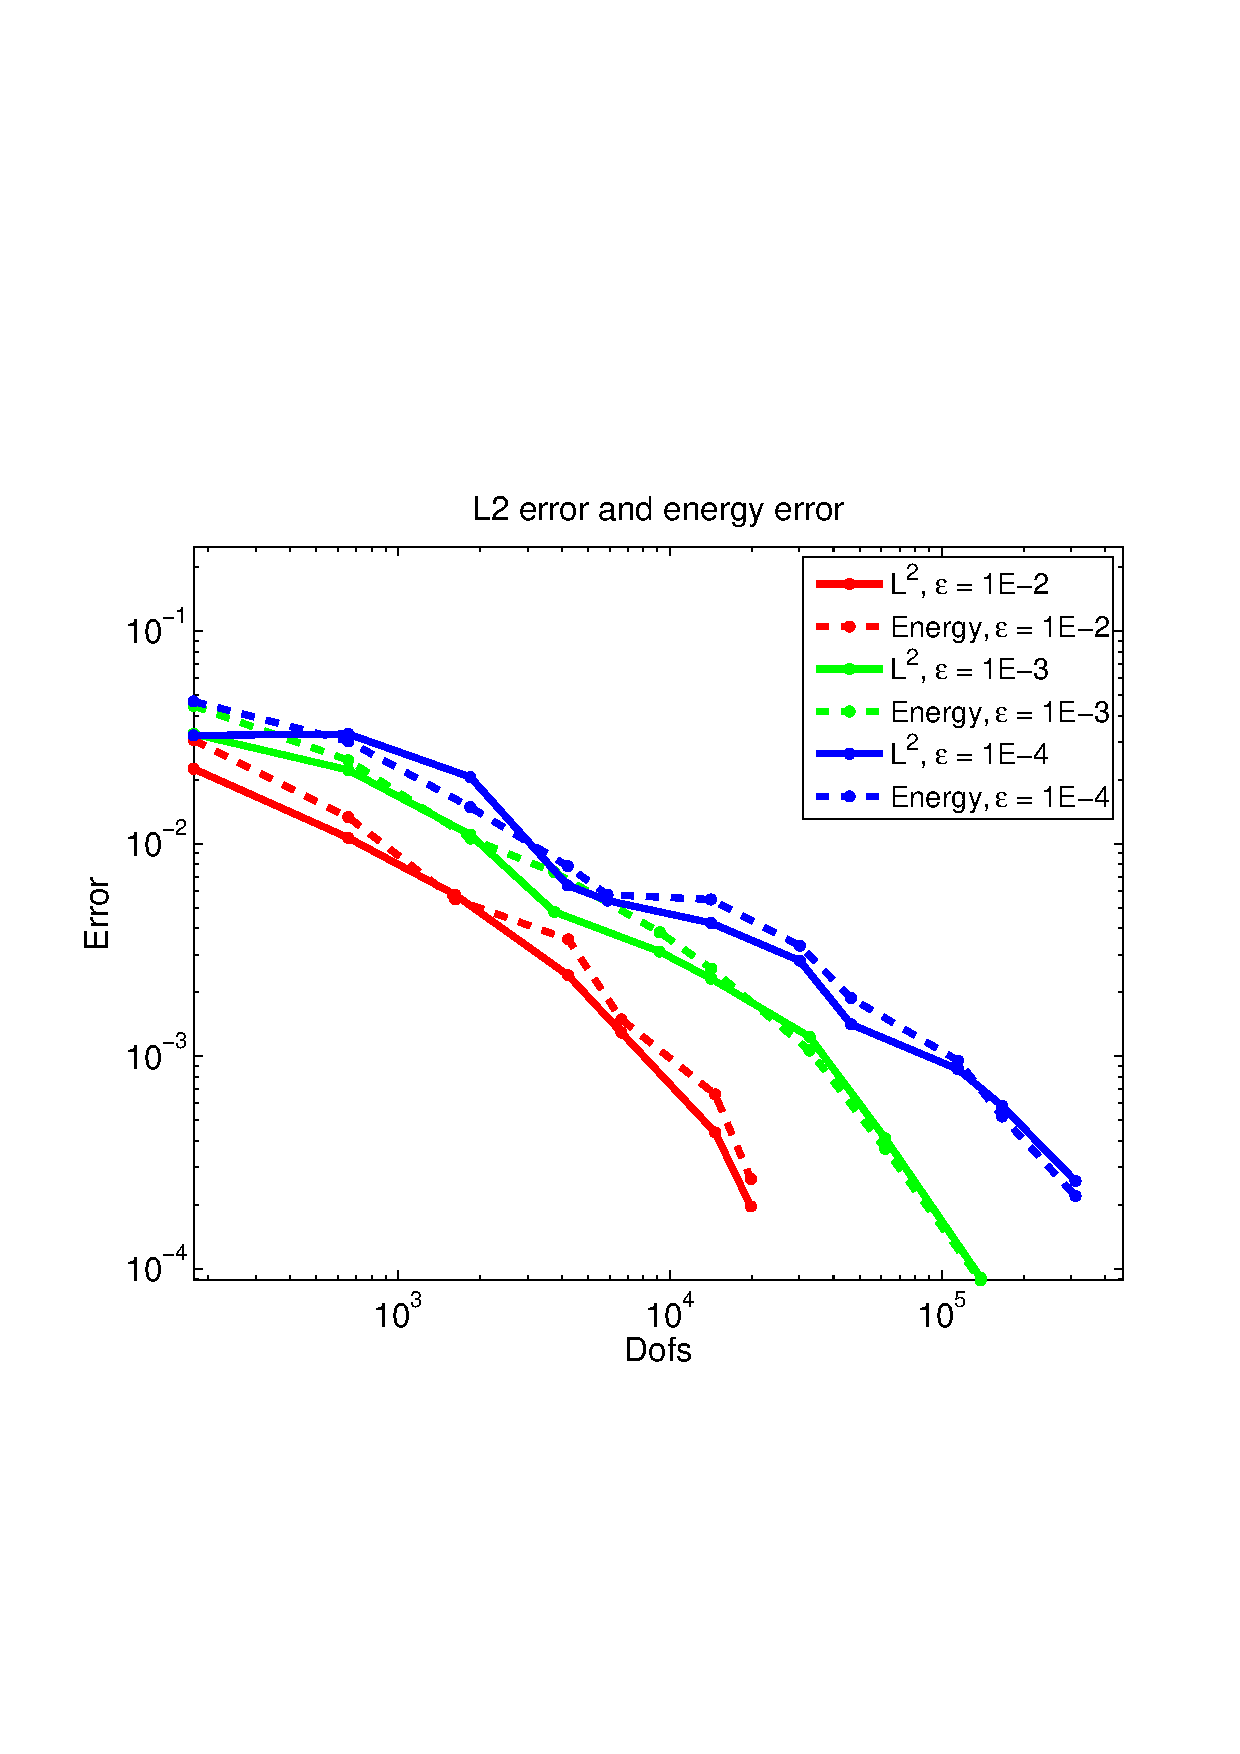
\includegraphics[scale=.36]{figs/rates_disc.png}
}
\subfigure{
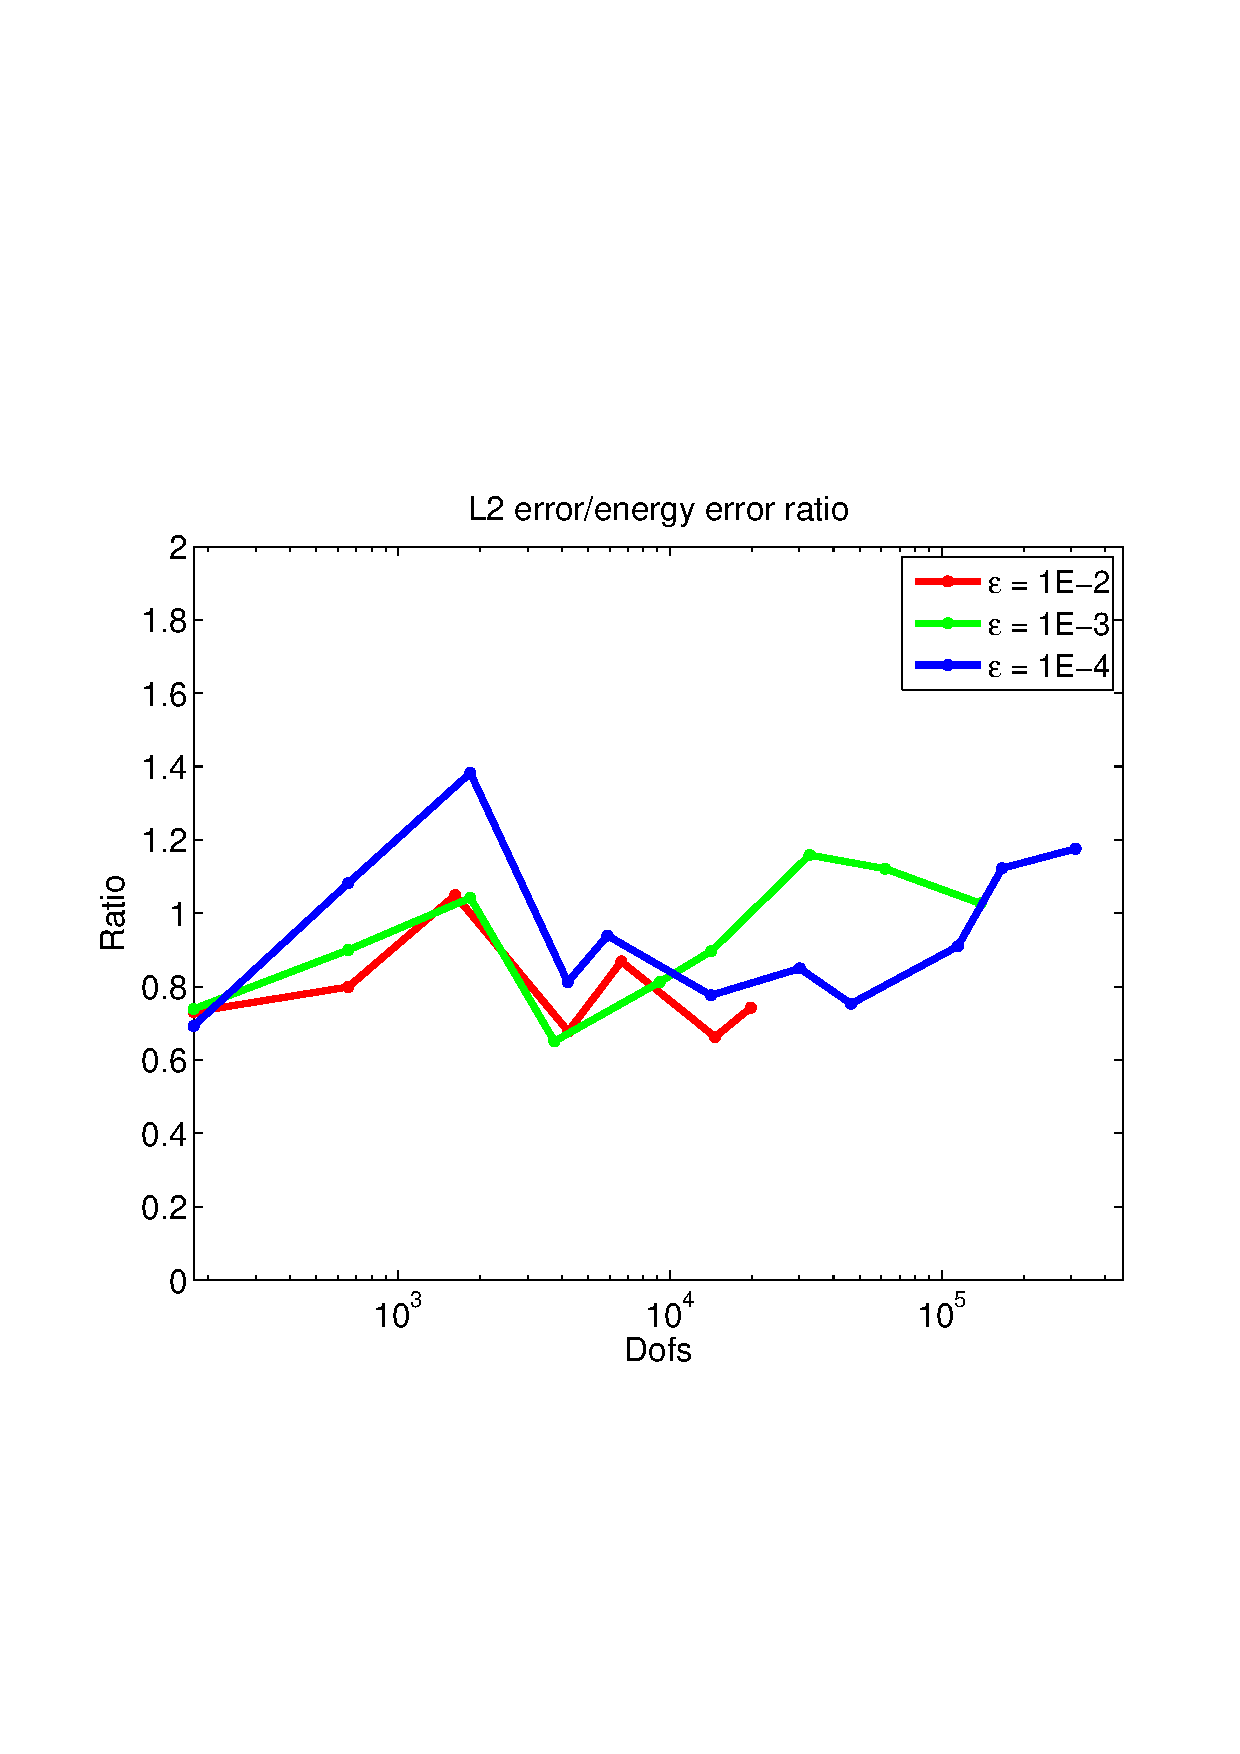
\includegraphics[scale=.36]{figs/ratio_disc.png}
}
\caption{$L^2$ and energy errors, and their ratio for $\epsilon=.01$, $\epsilon=.001$, $\epsilon=.0001$, with discontinuous $u_0$ approximated by a Fourier expansion. }
\label{disc_sol_fourier}
\end{figure}

The ratios of $L^2$ to energy error are now less predictable than for the previous example, in part due to the difficulty in approximating highly oscillatory boundary conditions. The numerical experiments were originally performed by applying boundary conditions via interpolation; the result was that the highly oscillatory inflow boundary condition was not sampled enough to be properly resolved, causing the solution to converge to a solution different than the exact solution.  The experiments were repeated using the penalty method to enforce inflow conditions; however, we note that the proper way to do so is to use an $L^2$ projection at the boundary.  Even when using the penalty method, however, the ratios still remain bounded and close to $1$ for $\epsilon$ varying over two orders of magnitude, as predicted by theory. 



\chapter{Extension to nonlinear problems and systems of equations}

\section{DPG for nonlinear problems}
\section{The viscous Burgers equation}

We will begin with the viscous Burgers' equation as an example of 

\begin{figure}[!h]
\centering
\includegraphics[scale=.5]{figs/burgers1e4.png}
\caption{Shock solution for Burgers' equation with $\epsilon = 10^{-4}$.} 
\end{figure}

\section{The compressible Navier-Stokes equations}

We briefly review the 2D compressible Navier-Stokes equations and formulate DPG for the nonlinear system. 
\begin{itemize}
\item \textbf{Conservation equations}
\begin{align*}
\div \vecttwo{\rho u_1 }{\rho u_2} &= 0\\
\div \vecttwo{\rho u_1^2+p }{\rho u_1 u_2} &= \div\left(\vec{\sigma_{i1}}\right)\\
\div \vecttwo{\rho u_1 u_2}{\rho u_2^2+p } &= \div\left(\vec{\sigma_{i2}}\right)\\
\div\vecttwo{((\rho e)+p)u_1}{((\rho e)+p)u_2} &= \div\left[\boldsymbol\sigma \boldsymbol u + \vec{q}\right],
\end{align*}
where $\boldsymbol \sigma$ is the stress tensor whose $ij$th term is $\sigma_{ij}$, and $\boldsymbol u$ is the vector $(u_1,u_2)^T$.  

\item \textbf{Newtonian fluid laws}

We represent $\boldsymbol\sigma$ using the Newtonian fluid law
\[
\sigma_{ij} = \mu(u_{i,j} + u_{j,i}) + \lambda u_{k,k} \delta_{ij}
\]
where $\mu$ is viscosity and $\lambda$ is bulk viscosity. 
%Following elasticity, a general formula for the stress tensor is 
%\[
%\sigma_{ij} = 2\mu \epsilon_{ij} + \lambda \epsilon_{kk} \delta_{ij}
%\]
We can invert the stress tensor under isotropic and plane strain assumptions to get
\[
\frac{1}{2}\left(\grad  \boldsymbol u + \grad ^T  \boldsymbol u\right) = \frac{1}{2\mu} \sigma_{ij} - \frac{\lambda}{4\mu (\mu + \lambda)} \sigma_{kk}\delta_{ij}
\]
We also have
\[
\frac{1}{2}\left(\grad  \boldsymbol u + \grad ^T  \boldsymbol u\right) = \grad  \boldsymbol u - \boldsymbol \omega
\]
where $\boldsymbol \omega$ is the antisymmetric part of the infinitesimal strain tensor:
\[
\boldsymbol \omega = \frac{1}{2}\left(\grad  \boldsymbol u - \grad ^T  \boldsymbol u\right).
\]
Thus our final form is
\begin{align*}
\grad  \boldsymbol u - \boldsymbol \omega = \frac{1}{2\mu} \boldsymbol \sigma - \frac{\lambda}{4\mu (\mu + \lambda)} { \rm tr}(\boldsymbol \sigma) \boldsymbol I.
\end{align*}
Notice that $\boldsymbol \omega$ is implicitly defined to be the antisymmetric part of $\grad u$ by taking the symmetric part of the above equation. 

We note that, though this is a standard approach in solid mechanics, it is nonstandard compared to the usual finite element and DG approaches to the viscous stresses. We adopt such an approach to better mirror our experiences with the convection-diffusion equation \cite{DPGrobustness,DPGrobustness2}. 

\item \textbf{Fourier's heat conduction law}

We assume Fourier's law 
\begin{align*}
\vec{q} &= \kappa \grad T,
\end{align*}
%where $\kappa$ is generally a function of temperature. 
We introduce here the Prandtl number here as well
\[
{\rm Pr} = \frac{\gamma c_v \mu}{\kappa}.
\]
In this case, we assume a constant Prandlt number, which implies that the heat conductivity $\kappa$ is proportional to viscosity $\mu$.

\end{itemize}

\subsection{Nondimensionalization}
To nondimensionalize our equations, we introduce nondimensional quantities for length, density, velocity, temperature, and viscosity. 
\[
\boldsymbol x^* = \frac{\boldsymbol x}{L}, \qquad \rho^* = \frac{\rho}{\rho_{\infty}}, \qquad u_1^* = \frac{u_1}{V_\infty}, \qquad u_2^* = \frac{u_2}{V_\infty}, \qquad T^* = \frac{T}{T_\infty}, \qquad \mu^* = \frac{\mu}{\mu_\infty}
\]
Pressure, internal energy, and bulk viscosity are then nondimensionalized with respect to the above variables
\[
p^* = \frac{p}{\rho_\infty V_\infty^2}, \qquad \iota^* = \frac{\iota}{V_\infty^2}, \qquad \lambda^* = \frac{\lambda}{\mu_\infty}
\]
We introduce, for convenience, the Reynolds number
\[
\Reyn = \frac{\rho_\infty V_\infty L}{\mu_\infty} 
\]
and the reference (free stream) Mach number
\[
M_\infty = \frac{V_\infty}{\sqrt{\gamma(\gamma-1)c_vT_\infty}}
\]
Note that 
\[
a = \sqrt{\frac{\gamma p_\infty}{\rho_\infty}} = \sqrt{{\gamma p_\infty}} = \sqrt{\gamma(\gamma-1)c_vT_\infty}
\]
The equations take the same form as before after nondimensionalization, so long as we define new material constants
\[
\tilde{\mu} = \frac{\mu^*}{\Reyn}, \qquad \tilde{\lambda} = \frac{\lambda^*}{\Reyn}, \qquad \tilde{c}_v = \frac{1}{\gamma(\gamma-1)M_\infty^2}, \qquad \tilde{\kappa} = \frac{\gamma\tilde{c}_v\tilde{\mu}}{\rm Pr}
\]
From here on, we drop the $^*$ superscript and assume all variables refer to their nondimensionalized quantities.

To summarize, our system of equations in the classical variables is now
\begin{align*}
\div \vecttwo{\rho u_1 }{\rho u_2} &= 0\\
\div \left(\vecttwo{\rho u_1^2+p }{\rho u_1 u_2} - \boldsymbol \sigma_{1}\right) &=0\\
\div \left(\vecttwo{\rho u_1 u_2}{\rho u_2^2+p } - \boldsymbol \sigma_{2}\right) &=0\\
\div \left(\vecttwo{((\rho e)+p)u_1}{((\rho e)+p)u_2} - \boldsymbol\sigma \mathbf{u} - \vec{q}\right) &=0\\
\frac{1}{2\mu} \boldsymbol \sigma - \frac{\lambda}{4\mu (\mu + \lambda)} { \rm tr}(\boldsymbol \sigma) \boldsymbol I &= \grad \mathbf{u} - \Reyn \, {\boldsymbol \omega}\\
\frac{1}{\kappa}\vec{q} &= \grad T
\end{align*}
We strongly enforce symmetry of the stress tensor $\boldsymbol \sigma$ by setting $\sigma_{21} = \sigma_{12}$. Additionally, we have scaled the antisymmetric tensor $\boldsymbol \omega$ by the Reynolds number to ensure that $\boldsymbol \omega = O(1)$ for all ranges of $\Reyn$.  

\subsection{Linearization}

As the equations for viscous compressible flow are nonlinear and cannot be solved exactly, we linearize the equations and adopt an iterative procedure for approximating the nonlinear solution.\footnote{We note that it is possible to linearize the strong form of the equations and then derive a linearized weak form, instead of linearizing the weak form of the nonlinear equations, which is done here.  The two formulations are equivalent; however, extraneous linearization of the fluxes is avoided using the latter approach.}  We outline the linearization of both the conservation and stress laws in this section.

\subsubsection{Conservation laws}

The Navier-Stokes conservation laws can be written as 
\begin{align*}
\div \vecttwo{\rho u_1 }{\rho u_2} &= 0\\
\div \left(\vecttwo{\rho u_1^2+p }{\rho u_1 u_2} - \boldsymbol \sigma_{1}\right) &=0\\
\div \left(\vecttwo{\rho u_1 u_2}{\rho u_2^2+p } - \boldsymbol \sigma_{2}\right) &=0\\
\div \left(\vecttwo{((\rho e)+p)u_1}{((\rho e)+p)u_2} - \boldsymbol \sigma_1 \cdot \boldsymbol u- \boldsymbol \sigma_2 \cdot \boldsymbol u - \vec{q}\right) &=0,
\end{align*}
where $\boldsymbol \sigma_1$ is the $i$th column or row of $\boldsymbol \sigma$, or more generally, if we group our Eulerian and stress variables into the vector variables $\boldsymbol U$ and $\boldsymbol \Sigma$, respectively
\[
\div (F_i(\boldsymbol U)-G_i(\boldsymbol U,\boldsymbol \Sigma) = 0, \qquad i = 1,\ldots, 4,
\]
where $F_i$and $G_i$ are given as
\begin{align*}
F_1 = \vecttwo{\rho u_1 }{\rho u_2}, \quad &G_1 = 0\\
F_2 = \vecttwo{\rho u_1^2+p }{\rho u_1 u_2},\quad &G_2 = \boldsymbol \sigma_{1}\\
F_3 = \vecttwo{\rho u_1 u_2}{\rho u_2^2+p }, \quad &G_3 = \boldsymbol \sigma_{2}\\
F_4 = \vecttwo{((\rho e)+p)u_1}{((\rho e)+p)u_2}, \quad &G_4 = \boldsymbol \sigma_1 \cdot \boldsymbol u + \boldsymbol \sigma_2 \cdot \boldsymbol u + \vec{q}
\end{align*}
The variational form restricted to a single element gives
\[
\langle \widehat{F}_i\cdot n, v\rangle - \int_K  (F(\boldsymbol U)-G_i(\boldsymbol U,\boldsymbol \Sigma)) \cdot \grad v_i = 0 , \qquad i = 1,\ldots, 4
\]
and the variational form over the entire domain is given by summing up the element-wise contributions. 

The presence of terms such as $\boldsymbol \sigma_i \cdot \boldsymbol u$ means that we will need to linearize in the stress variables $\sigma_ij$ in addition to our Eulerian quantities. Since fluxes and traces are linear functions of the unknowns, we do not need to linearize them. Instead, fluxes $\widehat{F}_{i,n}$ and traces $\widehat{u},\widehat{v},\widehat{T}$ will represent normal traces and traces of the accumulated nonlinear solution. The linearized variational formulation is thus
\begin{align*}
\langle \widehat{F}_i\cdot n, v\rangle &- \int_K  \left(F_{i,\boldsymbol U}(\boldsymbol U)\cdot \Delta \boldsymbol U -G_{i,\boldsymbol U}(\boldsymbol U, \boldsymbol \Sigma)\cdot \Delta \boldsymbol U - G_{i,\boldsymbol \Sigma}(\boldsymbol U, \boldsymbol \Sigma)\cdot \Delta \boldsymbol \Sigma \right)\cdot \grad v_i \\
&= \int_K  \left(F_i(\boldsymbol U)-G_i(\boldsymbol U)\right) \cdot \grad v_i \\
\qquad i &= 1,\ldots, 4
\end{align*}
where $F^i_{j,\boldsymbol U}$, $G^i_{j,\boldsymbol U}$, and $G^i_{j,\boldsymbol \Sigma}$ are the Eulerian and two viscous Jacobians (linearized w.r.t.\ the Eulerian/viscous variables), respectively.
%where
%\begin{align*}
%F^1_{1,\boldsymbol U} &= \{u,\rho ,0,0\} \\
%F^2_{1,\boldsymbol U} &= \{v,0,\rho ,0\} \\
%F^1_{2,\boldsymbol U} &=\left\{c_v T (\gamma -1)+u^2,2 u \rho ,0,c_v (\gamma -1) \rho \right\}\\
%F^2_{2,\boldsymbol U} &=\{u v,v \rho ,u \rho ,0\}\\
%F^1_{3,\boldsymbol U} &=\{u v,v \rho ,u \rho ,0\}\\
%F^2_{3,\boldsymbol U} &=\left\{c_v T (\gamma -1)+v^2,0,2 v \rho ,c_v (\gamma -1) \rho \right\}\\
%F^1_{4,\boldsymbol U} &=\left\{\frac{1}{2} u \left(2 c_v T (2 \gamma -1)+u^2+v^2\right),\frac{1}{2} \rho  \left(2 c_v T (2 \gamma -1)+3 u^2+v^2\right),u v \rho ,c_v u (2 \gamma -1) \rho \right\}\\
%F^2_{4,\boldsymbol U} &=\left\{\frac{1}{2} v \left(2 c_v T (2 \gamma -1)+u^2+v^2\right),u v \rho ,\frac{1}{2} \rho  \left(2c_v T (2 \gamma -1)+u^2+3 v^2\right),c_v v (2 \gamma -1) \rho \right\}
%\end{align*}
%The viscous Jacobians become (when linearized with respect to $\{\sigma_{11},\sigma_{12}, \sigma_{22}\}$)
%\begin{align*}
%G^1_{2,\boldsymbol \sigma} &= \{1,0,0\}\\
%G^2_{2,\boldsymbol \sigma} &= \{0,1,0\}\\
%G^1_{3,\boldsymbol \sigma} &= \{0,1,0\}\\
%G^2_{3,\boldsymbol \sigma} &= \{0,0,1\}\\
%G^1_{4,\boldsymbol \sigma} &= \{u_1,u_2,0\}\\
%G^2_{4,\boldsymbol \sigma} &= \{0,u_1,u_2\}
%\end{align*}
%and (when linearized with respect to the Eulerian variables)
%\begin{align*}
%G^1_{4,\boldsymbol U} &= \{0,\sigma_{11},\sigma_{12},0\}\\
%G^2_{4,\boldsymbol U} &= \{0,\sigma_{12},\sigma_{22},0\}
%\end{align*}

\subsubsection{Viscous equations}
We have two equations left to linearize - the constitutive laws defining our viscous stresses and heat flux terms. 
\begin{align*}
\frac{1}{2\mu}{\boldsymbol \sigma}- \frac{\lambda}{4\mu(\mu+\lambda)}{\rm tr}({\boldsymbol \sigma}){\boldsymbol I} + \Reyn {\boldsymbol \omega} &= 
\grad
\left[\begin{array}{c}
u_1\\
u_2
\end{array}
\right]\\
\frac{1}{\kappa}
\left[\begin{array}{c}
q_1\\
q_2
\end{array}\right] &=
\grad T
\end{align*}

We treat the first tensor equation as two vector equations by considering each column:
\begin{align*}
\frac{1}{2\mu} \vecttwo{\sigma_{11}}{\sigma_{12}} - \frac{\lambda}{4\mu(\mu+\lambda)}\vecttwo{\sigma_{11}+\sigma_{22}}{0} + \Reyn\vecttwo{0}{-\omega} - \grad u_1&= 0 \\
\frac{1}{2\mu} \vecttwo{\sigma_{12}}{\sigma_{22}} - \frac{\lambda}{4\mu(\mu+\lambda)}\vecttwo{0}{\sigma_{11}+\sigma_{22}} + \Reyn\vecttwo{\omega}{0} - \grad u_2 &= 0
\end{align*}
%These equations are linear in $\sigma_{ij}$, so the linearization is simple. 
Since all equations are linear in variables $q_1, q_2, w$ for all combinations of variables, we do not need to linearize any equations in $q_1, q_2, w$.  We do not linearize the viscosities $\mu$ and $\lambda$, but instead set them based on the power law and the solution at the previous timestep for simplicity. 

\subsection{Test norm}

%Recall the convection-diffusion problem 
%\begin{align*}
%\div \left(\beta u - \sigma\right) &= f\\
%\frac{1}{\epsilon}\sigma - \grad u &= 0.
%\end{align*}
%On domain $\Omega$, with mesh $\Oh$ and mesh skeleton $\Gh$, the DPG variational formulation is
%\begin{align*}
%b\left(\left(u,\sigma, \widehat{u}, \widehat{f}_n\right),
%\left( v, \tau \right)\right) = \left(u,\div \tau - \beta \cdot \grad
%v\right)_{\Oh} + \left(\sigma, \epsilon^{-1} \tau + \grad v\right)_{\Oh} - \LRa{
%\jump{\tau\cdot n}, \widehat{u} }_{\Gh} + \LRa{ \widehat{f}_n,
%  \jump{v} }_{\Gh}.
%\end{align*}
%with $v\in H^1$ and $\tau \in H({\rm div},\Oh)$. The test norm adopted for convection-diffusion in \cite{DPGrobustness2} is defined elementwise on $K$ as
%\[
%\|\left(v,\tau\right)\|_{V,K}^2 = \min\left\{\frac{\epsilon}{|K|},1\right\}\|v\|^2 + \epsilon \|\grad v\|^2 + \|\beta \cdot \grad v\|^2 + \| \div \tau-\beta\cdot\grad v\|^2 + \min\left\{\frac{1}{\epsilon},\frac{1}{|K|}\right\}\|\tau\|^2.
%\]
%This test norm both delivers robust control of the error in the $L^2$ variables $u$ and $\sigma$ and avoids boundary layers in the computation of local test functions. 

Recall that the test norm adopted for convection-diffusion is defined elementwise as
\[
\|\left(v,\tau\right)\|_{V,K}^2 = \min\left\{\frac{\epsilon}{|K|},1\right\}\|v\|^2 + \epsilon \|\grad v\|^2 + \|\beta \cdot \grad v\|^2 + \| \div \tau-\beta\cdot\grad v\|^2 + \min\left\{\frac{1}{\epsilon},\frac{1}{|K|}\right\}\|\tau\|^2.
\]
This test norm is extrapolated to the Navier-Stokes equations as follows: we denote the vector of $H^1$ test functions as $\boldsymbol V=\{v_1,v_2,v_3,v_4\}$, and similarly for $\boldsymbol W = \{\tau_1,\tau_2,\tau_3\}$. If $R_{\rm Euler}(\boldsymbol U,\boldsymbol \Sigma)$ and $R_{\rm visc}(\boldsymbol U,\boldsymbol \Sigma)$ are Eulerian and viscous nonlinear residuals, our formulation for the linearized Navier-Stokes equations can be written as
\begin{align*}
\div \left(A_{\rm Euler}\boldsymbol \delta U - A_{\rm visc}\boldsymbol \delta \Sigma\right) &= R_{\rm Euler}(\boldsymbol U,\boldsymbol \Sigma)\\
E_{\rm visc}\boldsymbol  \delta \Sigma - \grad \boldsymbol \delta U &= R_{\rm visc}(\boldsymbol U,\boldsymbol \Sigma)
\end{align*}
with variational formulation
\begin{align*}
\LRa{\widehat{F}_n,\boldsymbol V}_{\Gh} + \left(\boldsymbol \delta U,\div \boldsymbol W - A_{\rm Euler}^T\grad \boldsymbol  V\right) + \LRa{\widehat{\boldsymbol U},\boldsymbol W\cdot n}_{\Gh} + \left(\boldsymbol \delta \Sigma,E_{\rm visc}^T\boldsymbol W - A_{\rm visc}^T\grad \boldsymbol  V\right) &= 
\\ \LRa{R_{\rm Euler}(\boldsymbol U,\boldsymbol \Sigma),\boldsymbol V} + \LRa{R_{\rm visc}(\boldsymbol U,\boldsymbol \Sigma),\boldsymbol W}
\end{align*}
Identifying vector-valued terms in the Navier-Stokes formulation with equivalent scalar terms in the convection-diffusion equation allows us to extrapolate our test norm to systems of equations
\begin{align*}
\|\left(\boldsymbol V,\boldsymbol W\right)\|_{V, K}^2 =& \|\boldsymbol V\|^2 + \frac{1}{\Reyn} \|A_{\rm visc}^T\grad \boldsymbol V\|^2 + \|A_{\rm Euler}^T \grad \boldsymbol V\|^2 \\
& + \| \div \boldsymbol W - A_{\rm Euler}^T \grad \boldsymbol V\|^2 + \min\left\{\Reyn,\frac{1}{|K|}\right\}\|E_{\rm visc}^T\boldsymbol W\|^2.
\end{align*}
An advantage of this extrapolation approach is that the incompletely parabolic nature of the Navier-Stokes equation is taken into account; there is no diffusive term present in the mass conservation equation, and the test norm reflects that by requesting only limited regularity of $v_1$, the test function for the conservation equation.\footnote{The situation is analogous to using the full $H^1(\Oh)$ norm for the pure convection equation --- the optimal test norm $\nor{v}_V = \nor{\beta\cdot \grad v} + \nor{v}$ implies only streamline regularity, whereas taking $\nor{v}_V = \nor{\grad v} + \nor{v}$ implies stronger regularity on the test space $V$ than the graph norm. Consequently, convergence is suboptimal for DPG applied to the convection problem under the $H^1(\Oh)$ test norm.}

\subsection{Boundary conditions}

As a consequence of the ultra-weak variational formulation, our solution is linear in the flux and trace variables. Thus, the nonlinear boundary conditions can be applied directly to our fluxes $\widehat{f}_{i,n}, i = 1,\ldots,4$, and traces $\widehat{u}_1$, $\widehat{u}_2$, and $\widehat{T}$. Additionally, inflow boundary conditions are applied not directly to the trace variables $\widehat{u}_1$, $\widehat{u}_2$, and $\widehat{T}$, but to the fluxes $\widehat{f}_{i,n}$. Extrapolating from the convection-diffusion problem, this allows us to use a stronger test norm without experiencing adverse effects for smaller diffusion/higher Reynolds numbers, as described in Section~\secref{sec:testNormSec} and \cite{DPGrobustness,DPGrobustness2}.

\section{Nonlinear solver}

For our nonlinear solver, we use a pseudo-time stepping approach to iterate to a steady state solution, along with a greedy refinement scheme to eliminate spatial discretization error.  We cover briefly the details of the pseudo-timestepping method in this section.  
%Though we have not yet implemented adaptive timestepping, we are able to take large enough uniform timesteps over a coarse mesh such that convergence occurs sufficiently quickly.

\subsection{Pseudo-timestepping}

The solution of the compressible Navier-Stokes equations can be quite challenging; as mentioned previously, the direct application of a Newton algorithm often will not converge, especially for high Reynolds numbers.  Typically, a pseudo-timestepping algorithm is used in lieu of a full nonlinear Newton algorithm. The pseudo-timestep proceeds as follows: given the transient terms present in the conservation laws of compressible flow
\begin{align*}
\pd{\rho}{t} + \ldots \\
\pd{\LRp{\rho u}}{t} + \ldots \\
\pd{\LRp{\rho v}}{t} + \ldots \\
\pd{\LRp{\rho e}}{t} + \ldots,
\end{align*}
we discretize each time derivative using an implicit timestepping method.  Though second order time discretizations have been shown to be effective \cite{Demkowicz1990275, BenKirk}, we choose a first order backwards Euler discretization for simplicity.  Due to the fact that we've chosen to solve the Navier-Stokes equations under primitive variables $\rho, u, v$, and $T$, the time terms are nonlinear as well, and must be linearized.  After time discretization and linearization, we are left with a coupled system of reaction terms in the problem for our solution update at every timestep
\begin{align*}
A_{\rm time}\boldsymbol \delta U_i + \div \left(A_{\rm Euler}\boldsymbol \delta U_i - A_{\rm visc}\boldsymbol \delta \Sigma_i\right) &= R_{\rm Euler}(\boldsymbol U_i,\boldsymbol \Sigma_i) + R_{\rm time}(\boldsymbol U_{i-1},\boldsymbol U_i)\\
E_{\rm visc} \boldsymbol \Sigma_i - \grad \boldsymbol U_i &= R_{\rm visc}(\boldsymbol U_i,\boldsymbol \Sigma_i),
\end{align*}
where $R_{\rm time}(\boldsymbol U_{i-1},\boldsymbol U_i)$ is the transient residual.  Including the transient terms in our test norm as well, our final test norm is 
\begin{align*}
\|\left(\boldsymbol V,\boldsymbol W\right)\|_{V,K}^2 =& \nor{A_{\rm time}^T\boldsymbol V} + \|\boldsymbol V\|^2 + \frac{1}{\Reyn} \|A_{\rm visc}^T\grad \boldsymbol V\|^2 + \|A_{\rm Euler}^T \grad \boldsymbol V\|^2 \\
& + \| \div \boldsymbol W - A_{\rm Euler}^T \grad \boldsymbol V\|^2 + \min\left\{\Reyn,\frac{1}{|K|}\right\}\|E_{\rm visc}^T\boldsymbol W\|^2.
\end{align*}
Finally, convergence of the pseudo-timestepping method is determined by measuring the transient residual in the energy norm; in other words, we measure $\nor{e_{\rm time}}_V$, where
\[
\LRp{\LRp{\boldsymbol V,\boldsymbol W},\LRp{\boldsymbol dV,\boldsymbol dW}}_V = \LRp{R_{\rm time}(\boldsymbol U_{i-1},\boldsymbol U_i),\boldsymbol V}_{\L}, \quad \forall \LRp{\boldsymbol dV,\boldsymbol dW} \in V.
\]
The energy norm thus provides a consistent measure in which convergence of the nonlinear iteration at each timestep, convergence of the pseudo-timestepping algorithm to steady state, and nonlinear residual can all be assessed.  

\subsubsection{Dependence of solution on $dt$}

A surprising feature of pseudo-timestepping schemes for DPG is that, under the problem-dependent minimum-residual nature of the method, convergence to steady state can yield qualitatively slightly different solutions under different size timesteps.  We illustrate this using a ``plate'' example for convection-diffusion.  We consider the transient form of the conservation equation for convection-diffusion
\[
\pd{u}{t} + \div \LRp{\beta u - \sigma} = f, 
\]
where the stress law remains unchanged.  Applying a backwards Euler time discretization, at each timestep, we will solve for the current solution $u_i$ (as well as the current stress $\sigma_i$) given the previous timestep solution $u_{i-1}$ under
\[
\frac{u_i}{dt} + \div \LRp{\beta u_i - \sigma_i} = f + \frac{u_{i-1}}{dt}.
\]
The conserved flux $\beta_n u - \sigma_n$ is set to freestream values on the inflow, and 0 on the top boundary $y = 1$ and half of the bottom boundary $x < .5, y = 0$.  We set $u = 1$ for the boundary $x \in (.5,1), y = 0$. For this example, $\beta = (1,0)$ and $\epsilon = 10^{-3}$.  
\begin{figure}
\centering
\subfigure[$dt = .1$]{\includegraphics[width=2.5in]{dt10.png}}
\subfigure[$dt = .01$]{\includegraphics[width=2.5in]{dt100.png}}
\caption{Comparison of pseudo-timestepping to steady state for a convection-diffusion problem under two different sizes of timestep.}
\label{fig:dtComparison}
\end{figure}
This can be understood as the consequence of solving a ``moving target'' optimization problem -- our variational formulation and test norm for this problem are
\begin{align*}
\LRp{u_{i}, \frac{1}{dt}v}_{\L} + b\LRp{u_i,v} &= l(v) + \LRp{u_{i-1},\frac{1}{dt}v}_{\L}\\
\nor{\LRp{\tau,v}}_{V,dt}^2 &= \frac{1}{dt}\nor{v}_{\L}^2 + \nor{v}_V^2,
\end{align*}
where $\nor{\LRp{\tau,v}}_{V}$ is the test norm introduced in Section~\secref{sec:testNormSec}, and $b(u,v)$ and $l(v)$ are the bilinear form and load for the steady state form of the convection diffusion equation.  DPG solutions minimize the functional 
\[
J(u_i) = \sup_{v\in V} \frac{\LRp{u_{i}-u_{i-1}, \frac{1}{dt}v}_{\L} + b(u_i,v) - l(v)}{\LRp{\frac{1}{dt}\nor{v}_{\L}^2 + \nor{v}_V^2}^{\frac{1}{2}}}
\]
over a given mesh.  As $u_{i-1}\rightarrow u_{i}$, which we expect to happen as the pseudo-timestepping algorithm converges to steady state, the minimized functional becomes
\[
J(u_i) = \sup_{v\in V} \frac{b(u_i,v) - l(v)}{\LRp{\frac{1}{dt}\nor{v}_{\L}^2 + \nor{v}_V^2}^{\frac{1}{2}}}.
\]
While the transient portion of the residual disappears, a factor of $\frac{1}{dt}$ is still present in the test norm.\footnote{While the solution under smaller $dt$ appears to give visually higher quality results, we stress that simply adding the term $\frac{1}{dt}\nor{v}_{\L}$ to the test norm under the steady state version of the convection-diffusion equations does not achieve the same effect.  We are able to add this term without negative consequence due to the inclusion of the $\frac{u_i}{dt}$ term present in the variational formulation (see \cite{DPGrobustness,DPGrobustness2} for mathematical details).  Numerical experiments indicate that including $\alpha\nor{v}_{\L}$ in the test norm, where $\alpha > \frac{1}{dt}$, converges much more slowly to a fine-mesh reference solution than if $\alpha = \frac{1}{dt}$.}  Thus, we can expect that the nature of the steady state solution achieved through convergence of the pseudo-time algorithm can depend on the timestep $dt$.  We observe the same phenomena for analogous problems in compressible flow as well.  

\subsubsection{Adaptive time thresholding}

Adaptive timestepping (also known as pseudo-transient continuation) has been implemented successfully for problems in compressible flow \cite{BenKirk}. Typical adaptive time-stepping schemes modify the time-step based on some notion of the transient residual $R_i$ at timestep $i$, such that
\[
dt_{i+k} = \LRp{\frac{R_{i+k}}{R_i}}^r dt_i,
\]
where $r > 1$ dictates the rate of change of the timestep based on residual reduction, and $k$ indicates an integer interval at which to modify the timestep.  However, the minimum-residual nature of the DPG method and the ``moving target'' problem make the effectiveness of adaptive time-stepping schemes questionable.  

For our current experiments, we implement instead an adaptive time thresholding, where we adaptive decrease our convergence criterion based on the spatial energy error.  Recall that, under convergence of the pseudo-timestepping algorithm, the DPG energy error converges to the measure of the nonlinear residual in the dual norm.  We set convergence criterion for the pseudo-timestepping algorithm to be such that 
\[
\nor{e_{\rm time}}_V < \max \{\epsilon_t,\epsilon_{t,k}\},
\]
where $\epsilon_{t,k}$ is the tolerance at the $k$th refinement iteration, and $\epsilon_t < \epsilon_{t,k}$ is an absolute tolerance.  We initialize $\epsilon_{t,k}$ to $\epsilon_{t}$, then based on the energy error $\nor{u-u_h}_E$, we set 
\[
\epsilon_{t,k} = \alpha_t \nor{u-u_h}_E.
\]
Since the linearized error at a single timestep is composed of a sum of the linearization error, transient residual, and nonlinear residual, if the transient residual and linearization error are small, we expect that the nonlinear residual at that point will be sufficient to be an effective error indicator with which to drive adaptive mesh refinement.  In the following numerical experiments, $\alpha_t$ is set to $.005$.  

The aim of this adaptive thresholding is to relax the convergence criteria for solution of the nonlinear system at each refinement step such that the same refinement pattern is achieved with or without the use of adaptive time thresholding.  Numerical experiments seem to indicate that the same refinement pattern is produced with or without the implementation of this simple adaptive thresholding scheme, though wall-clock convergence times under adaptive thresholding are faster.  We hope to investigate both DPG-specific adaptive timestepping schemes and more advanced methods of balancing convergence criterion in the future.  

\subsection{Linear solver}

A clear choice for a linear solver under the ultra-weak variational formulation is static condensation, or the Schur-complement method. Given a block matrix structure of a stiffness matrix $K$, we can view the DPG system as
\[
Ku = \arr{A}{B}{B^T}{D}\vecttwo{u_{\rm flux}}{u_{\rm field}} = \vecttwo{f}{g} = l
\]
where $D$ has a block-diagonal structure, and $A$ and $D$ are both square matrices with $\dim{A} < \dim{D}$. This is due to the fact that, for the ultra-weak variational formulation (and for all HDG methods), the interior field degrees of freedom can be condensed out to yield a problem posed solely in terms of the coupled flux and trace degrees of freedom.  The system can be reduced to yield the condensed system
\[
\left(A-B D^{-1} B^T\right)u_{\rm flux} = f - B D^{-1} g
\]
where $D^{-1}$ can be inverted block-wise. Once the globally coupled flux and trace degrees of freedom are solved for, the field degrees of freedom can be reconstructed locally. An additional advantage of the above approach is that the Schur complement maintains the same sparsity pattern implied by the connectivity of the globally coupled flux and trace degrees of freedom.  Since the condensation process can be done locally, we can save memory by avoiding constructing the full stiffness matrix.

It has been shown that, unlike standard least-squares methods, DPG generates for the Poisson matrix a stiffness matrix with condition number $O(h^{-2})$ \cite{practicalDPG}. It is well known that, under standard finite element methods, if the condition number of the global stiffness matrix $K$ is $O(h^{-2})$, the condition number of the Schur complement is $O(h^{-1})$. Additionally, through either diagonal preconditioning or matrix equilibration, the condition number of the Schur complement can often be made significantly smaller than $O(h^{-1})$, and the positive-definiteness of the resulting system allows the use of iterative solvers in solving the condensed system.  Initial experiments indicate that, at least for quasi-uniform and low-order meshes, both algebraic multigrid and preconditioned conjugate gradients are able to solve the condensed system fairly rapidly.  We hope to experiment further with solvers for the condensed system, and to develop multigrid methods and preconditioners for adaptive and higher order meshes under DPG.  

\section{Test problems}

We applied the DPG method to two test problems in compressible flow -- flow over a flate plate, and flow over a compression ramp.  While the physics of both problems are fairly simple, they nonetheless display several features (shocks, singularities, boundary layers) that are computationally difficult to resolve without adaptivity.  Furthermore, the problems themselves are not usually solved without the aid of artificial or numerical diffusion and/or shock-capturing terms, which we eschew in our application of DPG to these model problems.

The numerical parameters used are as follows for:
\begin{itemize}
\item{DPG parameters:} $p = 2$ and $\Delta p = 2$ uniformly across the mesh. 
\item{Adaptivity parameters:} Energy threshold $\alpha$ for refinements is $\alpha = .4$ for the Carter flat plate example and $\alpha = .5$ for the Holden ramp example.  
\item{Time-stepping parameters:} Initial timestep $\Delta t = .1$, and initial tolerance for transient residual $\epsilon_t = 1e-7$.
\end{itemize}

Numerical experiments were run on a small cluster with 16 CPUs and 8GB memory, as well as on the Lonestar machine at the Texas Advanced Computing Center (TACC), using a varying number of cores, from 48 to 120 depending on problem geometry and parameters.  Experiments were done using the Camellia library \cite{Camellia}.
%Elements were partitioned using the Zoltan library of Trilinos \cite{ZoltanOverviewArticle}, using either a Hilbert space-filling curve or the REFTREE \cite{REFTREE} algorithm.  

\subsection{Numerical experiments: Carter flat plate}

The first problem of interest is the Carter flat plate problem \cite{Carter}. An infinitesmally thin flat plate disrupts a free stream flow, causing a shock to form at the tip of the plate, and a boundary layer forms and widens along the length of the plate.  

\begin{figure}
\centering
\includegraphics[width=3.5in]{flat_plate_BCs.pdf}
\caption{Carter flat plate problem.}
\end{figure}

\begin{enumerate}
\item \textbf{Symmetry boundary conditions:} $u_n = q_n = \pd{u_s}{n} = 0$. Here, this implies $u_2 = q_2 = \sigma_{12} = 0$. We impose the stress condition by noting that, for the flat plate geometry, if $u_2 = 0$, then at the top and bottom, with $n = (0,1)$, $\widehat{f}_{2,n} = \sigma_{12}$, and $\widehat{f}_{4,n} = q_2$ if $\sigma_{12}$ and $u_2 = 0$. They are applied here to the bottom free-stream boundary.
\item \textbf{Flat plate boundary conditions:} $u_1 = u_2 = 0$, and $T = T_w = \left[1+(\gamma-1)M_\infty^2/2\right] T_\infty = 2.8T_\infty$ (for Mach 3 flow). We impose these strongly on the trace variables $\widehat{u}_1, \widehat{u}_2, \widehat{T}$. 
\item \textbf{Symmetry boundary conditions} are applied also to the top free-stream boundary.
\item \textbf{Inflow boundary conditions:} free stream conditions are applied here to all four fluxes $\widehat{f}_{i,n}$.
\item \textbf{Outflow boundary conditions:} the exact boundary conditions to enforce here are not universally agreed on.  Many enforce $\pd{u_1}{n}=\pd{u_2}{n}=0$ and $\pd{T}{n} = 0$, while others enforce an outflow boundary condition only in regions where the flow is subsonic \cite{Demkowicz:1990:NFE:112271.112276}.  
We adopt a ``no boundary condition'' outflow condition, mimicing what is done in \cite{Shakib1991141}.%first introduced in \cite{FLD:FLD1650140506}. %A mathematical analysis and explanation of this boundary condition for standard $H^1$ elements is given in \cite{FLD:FLD505}. 
%An alternative boundary condition would be as follows: since $u_1$ and $u_2$ are not expected to be zero at these points, we can set $\widehat{f}_{2,n}$ and $\widehat{f}_{4,n}$ to their represented quantities using either the field variables from the background flow, or (in the case of pseudo-time stepping) the previous timestep's flux and field quantities. 
\end{enumerate}

We initialize our solution to
\[
\rho = 1,\qquad u_1= 1,\qquad u_2 = 0, \qquad T = 1%\frac{1}{\gamma(\gamma-1){\rm Ma}^2}
\]
which, we also take as the freestream values for the above variables, and is consistent with what was done by Demkowicz, Oden, and Rachowicz in \cite{Demkowicz1990275}. Stresses are set uniformly to zero.  We take the computational domain to be $\Omega = [0,2]\times[0,1]$. Under Dirichlet wall boundary conditions for all 3 traces $u_1$, $u_2$, and $T$, the solution develops a singularity in the density $\rho$ at the plate beginning, and both $T$ and $u_1$ form a boundary layer along the leading edge of the plate.  

\begin{figure}
\centering
\subfigure[$T$]{\includegraphics[width=2.5in]{T0.png}}
\subfigure[$u_1$]{\includegraphics[width=2.5in]{u0.png}}
\caption{Converged solution on 2 cells.}
\label{fig:Re1000_2cells}
\end{figure}

We perform 10 steps of adaptive mesh refinement, beginning with a mesh of only two square elements.  The solution on this coarsest mesh is given in Figure~\ref{fig:Re1000_2cells}, and the final solutions after 10 refinement steps are given in Figure~\ref{fig:Re1000}.  For this specific example, we use only isotropic refinements.  

\begin{figure}
\centering
\subfigure[$\rho$]{\includegraphics[width=2.8in]{rho.png}}
\subfigure[$u_1$]{\includegraphics[width=2.8in]{u1.png}}
\subfigure[$u_2$]{\includegraphics[width=2.8in]{u2.png}}
\subfigure[$T$]{\includegraphics[width=2.8in]{T.png}}
\caption{Solutions after twelve refinements for $p=2$ and $\Reyn = 1000$, starting from a mesh of 2 elements.}
\label{fig:Re1000}
\end{figure}

Typical coarse meshes for adaptive CFD computations aim to resolve, at least to some degree, the features of the solution; often, physical features such as high gradients are used to drive refinement.  For feature-based adaptivity to be effective, coarse mesh solutions must be of sufficiently high quality to resolve basic solution features.  Often, artificial diffusion and shock capturing must also be applied in order to produce visually clean solutions on underresolved meshes.  In contrast to this, the residual-based approach of DPG is able to place refinements accurately and efficiently despite the underresolution of solution features.  

Figure~\ref{fig:Re1000_midRefs} shows snapshots of the third and sixth steps of adaptive mesh refinement.  The main contribution to energy error is at the plate tip -- due to the change in boundary condition across the point $(.5,0)$, the viscous stresses are singular at this point (this is analogous to the convection-diffusion plate example given earlier).  Underresolution of the stresses at this point results in some pollution effects slightly upstream of the beginning of the plate; however, once $h\approx {\rm Re}^{-1}$ near the plate edge, these pollution effects disappear.  We observe numerically that decreasing $dt$ also limits how far upstream of the plate edge this pollution effect travels.

\begin{figure}
\centering
\subfigure[Mesh, 4th refinement]{\includegraphics[width=2.85in]{mesh4.png}}
\subfigure[$T$, 4th refinement]{\includegraphics[width=2.85in]{T4.png}}
\subfigure[Mesh, 8th refinement]{\includegraphics[width=2.85in]{mesh8.png}}
\subfigure[$T$, 8th refinement]{\includegraphics[width=2.85in]{T8.png}}
\caption{Snapshots of adaptive meshes and solutions for two different steps of adaptivity $\Reyn = 1000$.}
\label{fig:Re1000_midRefs}
\end{figure}

We observe numerically that $\rho$ also behaves singularly at the plate tip -- due to the presence of this strong singularity, the coloring of the wide range of values for $\rho$ in Figure~\ref{fig:Re1000} causes the solution to appears largely uniform, save for a flare up at the tip of the plate.  To better visualize density, $\rho$ is rescaled such that the features of the solution away from the singularity, as well as the final mesh after 10 refinement steps, are visible in Figure~\ref{fig:rhoScaled}.    

\begin{figure}
\centering
\subfigure[$\rho$]{\includegraphics[width=2.8in]{rhoRescaled.png}}
\subfigure[Mesh]{\includegraphics[width=2.8in]{mesh12.png}}
\caption{Rescaled solution for $\rho$ in the range $[\rho_{\min},2]$ and adaptive mesh after 12 refinement steps.}
\label{fig:rhoScaled}
\end{figure}

We can also zoom in on the plate tip to view the solution quality at the singular point.  Figure~\ref{fig:Re1000_zoom} demonstrates that the solution remains smooth and well-resolved at the plate tip, despite the presence of a singularity in the viscous stresses.%, and the fact that high order methods do not tend to resolve singularities as efficiently as low order methods \cite{hp1}.\cite{Optimal $hp$-adaptive strategies for elliptic problems with singularities result in meshes of lowest 

\begin{figure}
\centering
\subfigure[$\rho$]{\includegraphics[scale=.23]{rhoZoom.png}}
\subfigure[$u_1$]{\includegraphics[scale=.23]{u1Zoom.png}}
\subfigure[$u_2$]{\includegraphics[scale=.23]{u2Zoom.png}}
\subfigure[$T$]{\includegraphics[scale=.23]{TZoom.png}}
\caption{Zoom of solutions at the beginning of the plate for $p=2$ and $\Reyn = 1000$.}
\label{fig:Re1000_zoom} 
\end{figure}

We increased the Reynolds number to $10,000$ to assess the behavior of DPG for higher Reynolds numbers.  However, we found it necessary to modify the method in several ways in order to achieve satisfactory results.  

First, we implemented a line search algorithm to enforce positivity of both temperature and density, which are physically defined to be positive quantities.  Given updates $\triangle \rho$ and $\triangle T$, we update our previous solution by setting 
\begin{align*}
\rho \coloneqq \rho + \alpha_{\rm line}\triangle \rho \\
T \coloneqq T + \alpha_{\rm line}\triangle T,
\end{align*}
where $\alpha_{\rm line}$ is chosen, for some $\delta > 0$, such that
\begin{align*}
\rho + \alpha_{\rm line}\triangle \rho - \delta = 0\\
T + \alpha_{\rm line}\triangle T  - \delta = 0.
\end{align*}
Since the addition of a line search can slow the convergence of a nonlinear algorithm, we incorporate also a Newton iteration at each timestep to effectively solve the nonlinear system at each timestep.  We consider $\nor{\triangle U}_E < \epsilon_{\rm Newton}$ to be our condition for convergence of the Newton iteration, though we also limit the number of allowed Newton steps for computational efficiency.  The full solver algorithm is given in Algorithm~\ref{fig:algorithm}.  
\begin{algorithm}                      % enter the algorithm environment
\caption{Calculate $y = x^n$}          % give the algorithm a caption
\label{alg1}                           % and a label for \ref{} commands later in the document
\begin{algorithmic}                    % enter the algorithmic environment
\FOR{ number of refinement steps } 
    \WHILE{ $R_{\rm time} > \epsilon_t$}
        \STATE k = 0
        \WHILE{$\nor{\triangle U}_E > \epsilon_{\rm Newton}$ and $k <$ maximum Newton steps}
            \STATE Solve for $\triangle U$, determine $\alpha_{\rm line}$.  
            \STATE $U \coloneqq U + \alpha_{\rm line}\triangle U$.  
            \STATE k = k+1
        \ENDWHILE
        \STATE Increment timestep.  
    \ENDWHILE
    \STATE Compute energy error and refine based on a greedy refinement algorithm.
    \STATE Set $\epsilon_t = \alpha_t \nor{u-u_h}_E$.    
\ENDFOR
\end{algorithmic}
\caption{Pseudo-timetepping adaptive algorithm with line search.}
\label{fig:algorithm}
\end{algorithm}
For higher Reynolds numbers and highly refined meshes, the solution update exhibits large oscillations, such that the solution at a timestep can become negative, under which the pseudo-timestepping algorithm can stall or even diverge.\footnote{We note that these large oscillations mimic experiences in 1D as well, where the linearized solution was shown to exhibit sharp gradients near shocks that did not disappear, even with additional mesh refinement, indicating that the presence of such overshoots and undershoots is a consequence of the linearization, as opposed to the stability of the discretization \cite{NS_DPG1D}. This is discussed in more detail in Section~\secref{sec:oscillations}.  

We note also that theory developed in \cite{DPGrobustness2} for the convection-diffusion problem assumes a smooth convection field.  However, under linearization of the Burgers' and Navier-Stokes equations, the solution around which we linearize dictates the convection field, and can display large gradients.  While we have not observed issues in the Burgers' equation related to this, we hope to revisit the analysis done in \cite{DPGrobustness2} and generalize it for convection fields with large gradients.}.  However, we have observed that requiring a strictly positive solution appears to be too restrictive a constraint for some meshes; the use of line search does not appear to be necessary for convergence of the pseudo-timestepping algorithm on coarser meshes (until the 10th refinement iteration, or $h< .001$).  

Finally, we implement an ``effective'' CFL number; though implicit time integration schemes are unconditionally stable (compared to explicit schemes), a CFL condition relating the size of the time increment to the (minimum) mesh size is often still used in practice to improve convergence speed and stability of the numerical scheme \cite{Shakib1991141}.   Our CFL number is chosen to be 64.  We note that this CFL number is implemented for non-standard reasons.  In fact, DPG is able to solve the steady-state system directly without the use of pseudo-timestepping (direct Newton iteration).  However, as noted previously, the size of the timestep under which pseudo-timestepping converges greatly affects the qualitative nature of the solution.  Figure~\ref{fig:dtCompare} demonstrates the difference between convergence at large and small timesteps -- for $dt$ large relative to the mesh size, the solution experiences upstream ``pollution'' effects.  
\begin{figure}
\centering
\subfigure[$dt = \infty$ (Direct Newton)]{\includegraphics[width=2.8in]{dtInf.png}}
\subfigure[$dt = 1.0$]{\includegraphics[width=2.8in]{dtOne.png}}
\subfigure[$dt = .1$]{\includegraphics[width=2.8in]{dtTenth.png}}
\caption{Steady state solutions for ${\rm Re} = 10,000$ under three different timesteps on a $16\times 8$ uniform mesh.}
\label{fig:dtCompare}
\end{figure}
Due to the upstream ``pollution'' present in the solution for $dt \geq 1$, the adaptive mesh refinement algorithm tends to add extraneous refinements on elements adjacent to the boundary $y = 0$, $x\in (0,1)$.  Decreasing the timestep alleviates this issue somewhat; however, an overly small timestep requires a large number of iterations to converge.  The implementation of an effective CFL number aims to balance the size of the timestep with the mesh size.\footnote{An additional reason for the implementation of an effective CFL number is the conditioning of the local problem, which was discussed for the convection-dominated diffusion problem in \cite{DPG3}.  The main problem concerning conditioning of local problems is the way that different test terms behave as a function of local element size.  We illustrate this using the element Sobolev norm $\nor{v}_{H^1(K)} = \nor{v}_{\L} + \nor{\grad v}_{\L}$ -- $\nor{v}_{\L} = O(h^2)$ (where $h$ is the element size), while $\nor{\grad v}_{\L} = O(1)$.  Thus, as $h\rightarrow 0$, the Sobolev norm over a single element approaches the Sobolev seminorm and loses positive definiteness, resulting in a highly ill-conditioned system to solve.  The addition of a first-order pseudo-timestepping term allows us to increase the relative magnitude of $\nor{v}_{\L}$ with respect to $\nor{\grad v}_{\L}$ and avoid conditioning issues while maintaining robustness of the method.}  

We note that, even with all of the above modifications, the pseudo-timetepping adaptive algorithm with line search would sometimes failed to converge below $\epsilon_t$ for ${\rm Re} \geq 10,000$.  Figure~\ref{fig:nonconvergence} shows a plot of the transient residual after the 14th refinement step; while the residual initially decreases, it stalls at about $R_{\rm time} \approx 10^{-4}$.  
\begin{figure}
\centering
\subfigure[Non-convergence]{\includegraphics[width=2.5in]{oscillations1.pdf}}
\subfigure[Recovery of convergence]{\includegraphics[width=2.5in]{oscillations2.pdf}}
\caption{Stalling and recovery of the pseudo-timestep iteration for $\Reyn = 10000$.}
\label{fig:nonconvergence}
\end{figure}
An examination of the difference in the solutions between the final and $125$th timesteps shows that the nonconvergence of the transient residual is due to oscillations in the solution (primarily in $\rho$) slightly upstream to the plate edge.  Visually, the solution converges everywhere else, save for this area.  Such behavior is also observed in \cite{BenKirk}, where, at the change in boundary conditions between the free stream and flat plate, an oscillation was observed in the solution which prevented convergence of his pseudo-time algorithm.  His oscillations are of smaller magnitude ($O\LRp{10^{-6}}$ as opposed to $O\LRp{10^{-4}}$), which may be the result of several differences between the methods presented.\footnote{Apart from the use of a standard Galerkin (continuous as opposed to discontinuous Galerkin) formulation, Kirk's approach differed from ours in the use of linear elements and the addition of artificial diffusion shock-capturing terms, both of which could explain the lower point at which error stagnates. Reasons for this loss of convergence in the pre-asymptotic range should be explored further.}  However, we note that, under additional refinements and increased resolution of the solution, the transient residual once again decreases in a smooth monotonic fashion, as shown in Figure~\ref{fig:nonconvergence}. 

\begin{figure}
\centering
\subfigure[$\rho$]{\includegraphics[width=2.8in]{rhoRe4Plate.png}}
\subfigure[$u_1$]{\includegraphics[width=2.8in]{u1Re4Plate.png}}
\subfigure[$u_2$]{\includegraphics[width=2.8in]{u2Re4Plate.png}}
\subfigure[$T$]{\includegraphics[width=2.8in]{TRe4Plate.png}}
\caption{Solutions after 18 refinements for $p=2$ and $\Reyn = 10000$.}
\label{fig:Re10000}
\end{figure}

For additional computational efficiency, we also implemented an anisotropic refinement scheme.  In 2D, the boundary layer is a primarily 1D phenomena, which we expect to be far better resolved by anisotropic refinement than by isotropic refinement.  We experimented first using the scheme described in Section~\secref{sec:aniso} as an anisotropy indicator; however, the anisotropic scheme appeared to be too conservative near the boundary layer, placing primarily isotropic refinements.  We modified our scheme in two ways -- first, we incorporated spatially variable thresholding.  Typically, anisotropic refinement in the $x$ direction is chosen if $e_{x,K} > \epsilon_r e_{y,K}$ (and vice versa for anisotropic refinement in the $y$-direction), where $e_{x_i,K}$ is the error in the $x_i$ direction.  We set $\epsilon_r = \epsilon_{r,K}$; in other words, we allow our anisotropic threshold to vary element-by-element, and decrease it from $\epsilon_r= 10$ to $\epsilon_{r,K} = 2.5$ for elements adjacent to the wall upon which the boundary layer forms.  Additionally, since the boundary layer typically displays rapid variation in the $y$-direction (the direction orthogonal to the wall), we relax the condition under which a vertically cut anisotropic refinement occurs to
\[
2 e_{y,K} > \epsilon_{r,K} e_{x,K}.
\]
Despite the artificial modification of the anisotropic refinement scheme, the resulting meshes still resolve boundary layer solutions more efficiently than isotropic refinements.  We hope to investigate reasons for the ineffectiveness of the pure anisotropic scheme for the compressible Navier-Stokes equations in future research.  

\begin{figure}
\centering
\subfigure[$\rho$]{\includegraphics[width=2.8in]{rhoRescaledRe4Plate.png}}
\subfigure[Mesh]{\includegraphics[width=2.8in]{meshRe4Plate.png}}
\caption{Rescaled solution for $\rho$ in the range $[\rho_{\min},2]$ and adapted mesh.}
\label{fig:rhoScaled}
\end{figure}

\begin{figure}
\centering
\subfigure[$\rho$]{\includegraphics[width=2.8in]{rhoZoomRe4Plate.png}}
\subfigure[$u_1$]{\includegraphics[width=2.8in]{u1ZoomRe4Plate.png}}
\subfigure[$u_2$]{\includegraphics[width=2.8in]{u2ZoomRe4Plate.png}}
\subfigure[$T$]{\includegraphics[width=2.8in]{TZoomRe4Plate.png}}
\caption{Zoom of solutions at the beginning of the plate for $p=2$ and $\Reyn = 10000$.}
\label{fig:Re1e4Zoom}
\end{figure}

We note that the resolution of the solution near the plate edge in Figure~\ref{fig:Re1e4Zoom} for Reynolds number 10000 is qualitatively rougher than that for Reynolds 1000 in Figure~\ref{fig:Re1000_zoom}; this is due to the greedy refinement algorithm emphasizing refinements most strongly at the singular point and not in shock resolution, as well as the fact that at a higher Reynolds number, the shock width is thinner and more difficult to resolve.  Further refinement steps improve resolution of the shock features.  

%\begin{figure}[!h]
%\centering
%\subfigure[${\rm Re} = 1000$]{\includegraphics[scale=.5]{figs/Re1000p2/heatflux.png}}
%\subfigure[${\rm Re} = 10000$]{\includegraphics[scale=.3]{figs/Re1e5/q2line.png}}
%\caption{Heat flux at the bottom boundary.}
%\end{figure}

\subsection{Holden ramp problem}

Our second problem is a modified version of the Holden ramp problem, which models supersonic/hypersonic flow over a compression corner (the geometry of which is given in Figure~\ref{fig:holdenCartoon}).  Similarly to the Carter flat plate problem, a flat plate disrupts the flow and forms a weak shock at the plate tip due to viscous effects and no-slip boundary conditions.  The boundary layer grows down the plate edge, deflecting upwards due to the presence of the compression corner.  A stronger shock forms slightly upstream of the compression corner in order to deflect the incoming supersonic flow, and is a common test problem for adaptive finite element methods for compressible flow \cite{Rachowicz1997231,Barter,BenKirk}.  

\begin{figure}
\centering
\includegraphics[width=4in]{holden.pdf}
\caption{A modification of the Holden ramp/compression corner problem.}
\label{fig:holdenCartoon}
\end{figure}

The original plate length is given to be .442, while the ramp length is given to be .269. We have modified the problem slightly in order to exactly represent the boundary conditions on a coarse mesh while keeping the ratio of plate length to ramp length roughly the same. Similarly to the Carter flat plate, we start out with a very coarse $2 \times 3$ mesh of 6 elements.  We initialize our solution to the freestream values
\[
\rho_{\infty} = 1,\qquad u_{1,\infty}= 1,\qquad u_{2,\infty} = 0, \qquad T_{\infty} = 1
\]
and again set stresses uniformly to zero.   

\begin{figure}
\centering
\subfigure[$\rho$ rescaled]{\includegraphics[width = 2.9in]{rhoRescaledMa6Ramp.png}}
\subfigure[$u_1$]{\includegraphics[width = 2.9in]{u1Ma6Ramp.png}}
\subfigure[$u_2$]{\includegraphics[width = 2.9in]{u2Ma6Ramp.png}}
\subfigure[$T$]{\includegraphics[width = 2.9in]{TMa6Ramp.png}}
\subfigure[Mesh]{\includegraphics[width = 5.5in]{meshMa6Ramp.png}}
\caption{Solutions and adaptive mesh for ${\rm Ma} = 6$ and $\Reyn = 10000$.}
\label{fig:holdenMa6}
\end{figure}

We first solve under Mach 6 flow.\footnote{The increase in Mach number is to change the angle of the shock; under the current setup, Mach 3 flow produced a shock which reflected off the top boundary $y = 1$  We note that the effect of Mach number under our nondimensionalization of choice is to decrease the thermal diffusivity constant $\kappa$ relative to the viscosities $\mu$ and $\lambda$.} and Reynolds number of 10,000, or a Reynolds number of 33,936 if measured with respect to the original plate length of .442.  The wall temperature is set to $T_{w} = 2.8T_{\infty}$, identically to the flat plate problem.  24 mesh refinements were performed, resulting in a final mesh of 1858 elements.  Figure~\ref{fig:holdenMa6} shows both solution values and final adaptive mesh.  Due to a large maximum value of $\rho_{\max} = 14.1538$ at the plate tip, the resulting solution for $\rho$ is scaled to better show qualitative features of the flow.  The presence of the second shock deflecting the incoming supersonic flow at the ramp is clearly seen in both the solutions and the adaptive mesh refinements.  

\begin{figure}
\centering
\subfigure[Initial mesh]{\includegraphics[width = 2.9in]{rampMesh0.png}}
\subfigure[6 refinements]{\includegraphics[width = 2.9in]{rampMesh6.png}}
\subfigure[12 refinements]{\includegraphics[width = 2.9in]{rampMesh12.png}}
\subfigure[18 refinements]{\includegraphics[width = 2.9in]{rampMesh18.png}}
\caption{Sequence of adaptive meshes for ${\rm Ma} = 6$ and $\Reyn = 10000$.}
\label{fig:holdenMa6Meshes}
\end{figure}

We can examine the sequence of adaptive meshes generated by the DPG method.  Figure~\ref{fig:holdenMa6Meshes} shows the initial mesh, as well as the 6th, 12th, and 18th subsequent refinements generated automatically by the DPG method.  Unlike the previous sequence of meshes generated by the flat plate example, refinements tend to be placed most heavily near the shock at the outflow ramp.  By the 18th refinement, the adaptive mesh looks qualitatively very similar to the final mesh of 24 refinements, and further refinements focus on the resolution of the shocks originating at the plate edge and at the ramp outflow.  

\begin{figure}
\centering
\subfigure[$\rho$ rescaled]{\includegraphics[width = 2.9in]{rhoRescaledshockMa6Ramp.png}}
\subfigure[$T$]{\includegraphics[width = 2.9in]{TshockMa6Ramp.png}}
\subfigure[Mesh]{\includegraphics[width = 4in]{shockMeshMa6Ramp.png}}
\caption{Zoom of solutions and adaptive mesh around shock. }
\label{fig:holdenMa6Zoom}
\end{figure}

Figure~\ref{fig:holdenMa6Zoom} shows a zoom of the second stronger shock that develops near the ramp outflow.  Refinements are placed very heavily near the shock, which we expect due to the fact that a shock forms a stronger gradient than a boundary layer.  We note that our residual-driven adaptivity scheme places mesh refinements in a very precise manner; refinements on ramp boundary are placed slightly more heavily upstream than downstream.  We believe this is due to the fact that solution gradients are slightly higher in $\rho$ at the upstream section of the ramp.  

\begin{figure}
\centering
\subfigure[$\rho$ rescaled]{\includegraphics[width = 2.9in]{rhoRescaledMa11Ramp.png}}
\subfigure[$u_1$]{\includegraphics[width = 2.9in]{u1Ma11Ramp.png}}
\subfigure[$u_2$]{\includegraphics[width = 2.9in]{u2Ma11Ramp.png}}
\subfigure[$T$]{\includegraphics[width = 2.9in]{TMa11Ramp.png}}
\subfigure[Mesh]{\includegraphics[width = 5.5in]{meshMa11Ramp.png}}
\caption{Solutions and adaptive mesh for ${\rm Ma} = 11.68$ and $\Reyn = 16442.4$.}
\label{fig:holdenMa11}
\end{figure}

The second set of conditions under which we solve are under Mach 11.68 flow and Reynolds number of 16,4	42.4, or 55,800 if measured with respect to original plate length, with the wall temperature set to $T_{w} = 4.6T_{\infty}$.  24 automatic mesh refinements are performed under an energy threshold of $.5$, resulting in a final mesh of 2385 elements.  

Figure~\ref{fig:holdenMa11} shows the resulting solution and final adaptive mesh.  The increased Mach number changes again the angle of the weak shock resulting from the change in boundary conditions at the plate edge.  Compared to the previous case of Mach 6 flow, where only 18 refinements steps were performed, 24 refinements were performed for the Mach 11.68 case, leading to a more highly resolved solution, especially near the plate tip.  Due to a large maximum value of $\rho_{\max} = 50.1805$ at the plate tip, the resulting solution for $\rho$ is scaled to better show qualitative features of the flow.  

%We note that, under a higher Mach number, the placement of adaptive mesh refinements appears to improve.  The element size adjacent to the plate tip for the Mach $6$ case is $h = O\LRp{10^{-4}}$, while the size of elements adjacent to the plate tip in the Mach 11 case is $h = O\LRp{10^{-5}}$.  For the Mach $6$ and Reynolds $10,000$ case of the ramp problem, several extraneous refinements were placed slightly upstream of the plate tip, corresponding to the location of large gradients in the Newton solution update.  More study is necessary to determine the reasons for the difference in behavior of the automatic adaptivity algorithm.
%
%\begin{figure}[!h]
%\centering
%%\subfigure[$\rho$]{\includegraphics[width = 2.9in]{rhoshock.png}}
%%\subfigure[$T$]{\includegraphics[width = 2.9in]{Tshock.png}}
%\subfigure[Mach 6]{\includegraphics[width = 2.75in]{plateMesh.png}}
%\subfigure[Mach 11]{\includegraphics[width = 2.75in]{plateMesh.png}}
%\caption{Zoom of solutions and adaptive mesh around the plate tip.}
%\label{fig:plateComparison}
%\end{figure}

\begin{figure}
\centering
\subfigure[$\rho$ rescaled]{\includegraphics[width = 2.9in]{rhoshockMa11Ramp.png}}
\subfigure[$T$]{\includegraphics[width = 2.9in]{TshockMa11Ramp.png}}
\subfigure[Mesh]{\includegraphics[width = 4in]{shockMeshMa11Ramp.png}}
\caption{Zoom of solutions and adaptive mesh around shock. }
\label{fig:holdenMa11Zoom}
\end{figure}

Compared to the Mach 6 case, where 18 refinements were performed, the resolution of the mesh near the shock at the ramp outflow for Mach 11.68 flow and 18 refinements is qualitatively similar.  Further refinement steps increase resolution of the mesh near the shock, as shown in Figure~\ref{fig:holdenMa11Zoom}.  

Finally, we plot the normal heat flux over the plate and ramp for both Holden problems in Figure~\ref{fig:heatFlux}.  The normal heat flux over the flat plate is indicated by the blue line, while the dotted brown line indicates the heat flux over the ramp, and both are plotted against the x-coordinate along the plate/ramp boundary.  The normal heat flux is given by the normal trace of the conserved quantity in the energy equation
\[
\widehat{f}_{4,n} = (\rho e+p)u_n - \boldsymbol n\cdot \boldsymbol \sigma\cdot \boldsymbol u + q_n.
\]
Recognizing that $u_1 = u_2 = 0$ reduces the above to $\widehat{f}_{4,n} = q_n$.  

The heat flux develops a strong singularity at the point $(-.5,0)$, where the boundary condition changes from a Neumann/stress boundary condition to a Dirichlet/no-slip boundary condition.\footnote{Figure~\ref{fig:heatFlux} cuts off this singularity in order to show the qualitative behavior of $q_n$ over the remainder of the boundary.  The maximum visualized values in the singular portion of $q_n$ are .35 for Mach 6 flow and 1.268 for Mach 11.68 flow.}  It can be shown that the Laplace equation develops a singularity in stress at under any such change in boundary conditions, and the same phenomena is observed for a similar setup under convection-diffusion \cite{localConservationDPG}.  

\begin{figure}
\centering
\subfigure[Mach 6, Reynolds 10,000]{\includegraphics[width=2.9in]{heatFluxMa6Ramp.png}}
\subfigure[Mach 11.68, Reynolds 16,442.4]{\includegraphics[width=2.9in]{heatFluxMa11Ramp.png}}
\caption{Normal heat flux $q_n$ over plate and ramp for the Holden problem.  The blue line indicates $q_n$ over the flat plate, while the brown line indicates $q_n$ over the ramp. }
\label{fig:heatFlux}
\end{figure}

\subsection{Higher Reynolds numbers}
\seclab{sec:oscillations}
For higher Reynolds number, the pseudo-timestepping, we have encountered difficulties which have made it difficult to converge to a steady-state solution, even under the addition of an effective CFL number and line search to enforce positivity of density $\rho$ and temperature $T$.  However, we believe these difficulties to be related to the nature of the equations, rather than the robustness of the method.  We illustrate this with a simple example.  

Let us consider the 1D steady state viscous Burgers' equation on $[-\infty,\infty]$
\[
u\pd{u}{x} - \epsilon \pdd{u}{x} = 0.
\]
The exact solution to this equation under boundary conditions
\begin{align*}
u(-\infty) &= 1\\
u(\infty) &= -1
\end{align*}
can be easily derived (see \cite{Barter} for a simple derivation), and the solution and its first two derivatives are
\[
u(x) = \frac{1-e^{\frac{x}{\epsilon}}}{1+e^\frac{x}{\epsilon}}, \qquad u'(x) = \frac{-2e^{\frac{x}{\epsilon}}}{\LRp{1+e^{\frac{x}{\epsilon}}}^2\epsilon}, \qquad u''(x) = \frac{-2e^{\frac{x}{\epsilon}}\LRp{e^{\frac{x}{\epsilon}}-1}}{\LRp{1+e^{\frac{x}{\epsilon}}}^3\epsilon^2}
\]
\begin{figure}
\centering
\subfigure[$u(x)$]{\includegraphics[width = 1.8in]{u.pdf}}
\subfigure[$u'(x)$]{\includegraphics[width = 1.8in]{du.pdf}}
\subfigure[$u''(x)$]{\includegraphics[width = 1.8in]{ddu.pdf}}
\caption{$u(x)$ and its derivative and second derivative for $\epsilon = .01$.}
\label{fig:burgersSoln100}
\end{figure} 
Figure~\ref{fig:burgersSoln100} shows each of these functions for $\epsilon = .01$.  From the form of $u'(x)$ and $u''(x)$, we know these oscillations will grow rapidly as $\epsilon$ decreases.  Consider now the linearized Burgers' equation
\[
\pd{u\Delta u}{x} - \epsilon \pdd{\Delta u}{x} = - r(x)
\]
where $r(x) = u\pd{u}{x} - \epsilon \pdd{u}{x}$ is the strong form of the nonlinear residual.  Recall that for a pure Newton iteration, $u(x)$ is assumed to be known, and the linearized problem is driven by the residual.  The solution $u(x)$ is updated $u \coloneqq u + \Delta u$, and is repeated until $\Delta u$ and $r(x)$ are both approximately zero.

Let $u_\epsilon(x)$ be the exact solution for a particular viscosity $\epsilon$, and consider the setting of $u(x) = u_{\alpha \epsilon}(x)$, with $\alpha > 1$.  In other words, the initial guess for the Newton iteration is taken to be the exact solution for the viscous Burgers' equation under a larger viscosity (a less sharp shock), a method known as continuation (specifically, continuation in viscosity $\epsilon$).\footnote{We note that continuation in Reynolds number was attempted for the Navier-Stokes equations; however, the presence of large oscillations in the Newton update on highly adapted meshes caused the line search to return a near-zero step length, which stalled the nonlinear iteration prior to convergence to a steady state solution.}

\begin{figure}
\centering
\subfigure[$\epsilon = .01$]{\includegraphics[width = 2.5in]{residual100.pdf}}
\subfigure[$\epsilon = .001$]{\includegraphics[width = 2.5in]{residual1000.pdf}}
\caption{Residual for Burgers' equation with viscosity $\epsilon$ under the exact solution for ${2\epsilon}$.}
\label{fig:burgersResidual}
\end{figure} 

We plot $r(x)$ for $u(x) = u_{2\epsilon}(x)$ in Figure~\ref{fig:burgersResidual}.  While the form of the exact linearized solution $\Delta u$ is unknown, we see that the forcing term in the above equation develops oscillations that grow in magnitude and decrease in support as $\epsilon$ decreases.  We have observed similar behaviors for discretized solutions to the Burgers' and Navier Stokes equations -- the discrete linearized solution will develop gradients as well, though their magnitude will be limited by the resolution of the mesh.  However, additional refinements near shocks will introduce additional oscillations, which are subsequently damped by additional Newton iterations.  

In other words, not all oscillations are related to the method of discretization -- the exact linearized solution itself contains large oscillations, which are picked up more and more strongly in a discrete scheme as the mesh resolution approaches the viscous length scale $\epsilon$ (see \cite{DPGspacetime, DPGNS_1d} for additional numerical examples).  We note that these large oscillations are not an issue for the viscous Burgers' equation, as there is no positivity constraint on $u$.  However, as noted previously, the convergence of the nonlinear iteration for the compressible Navier-Stokes equations can stall or even diverge for sufficiently negative values of $\rho$ and $T$, which happens easily in the presence of large oscillations.  When a line search is implemented to enforce a strictly positive solution, the nonlinear iteration can stall, and numerical experiments have generated cases in which the line search length goes to zero, returning an under-converged solution.  

There are several approaches to controlling the magnitude of oscillations in the linearized solution -- a simple option is decreasing the size of the timestep; however, doing so can cause the number of iterations required for convergence to greatly increase.  The application of artificial diffusion near sharp gradients is another way in which to control such oscillations; however, this results in a modified set of equations, and, though solutions with contemporary artificial viscosity methods can produce solutions with expected qualitative features, there is a wide range of choices for artificial diffusion, and it was not clear in the scope of this paper which artificial viscosity method would be quantifiably superior, or most suitable for use with the DPG method.  


%\section{Area requirements}
\seclab{sec:proposedWork}

\subsection{Area A: Applicable mathematics}

\begin{itemize}
\item{\textbf{Completed: Prove robustness of DPG method for the scalar convection-diffusion problem.}}

Analysis has been done in \cite{DPGrobustness2}, extending the results of \cite{DPGrobustness}. In particular, we have introduced a test norm under which the DPG method robustly bounds the $L^2$ error in the field variables $u$ and the scaled stress $\sigma$. Numerical results confirm the theoretical bounds given. 

\item{\textbf{Proposed: Attempt analysis of the linearized Navier-Stokes system.}}

We hope to analyze the linearized Navier-Stokes equations to determine an optimal extrapolation of the test norm for the scalar convection-diffusion problem to systems. 

\end{itemize}

\subsection{Area B: Numerical analysis and scientific computation}

\begin{itemize}
\item{\textbf{Completed: Collaborative work with Nathan Roberts on the higher order parallel adaptive DPG code Camellia.}}

Most numerical experiments have been done using the higher-order adaptive codebase Camellia, built upon the Trilinos library and designed by Nathan Roberts. The library allows for rapid implementation of problems through a symbolic syntax similar to the Fenics project. Work has been done to support arbitrary-irregularity refinements in both $h$ and $p$, and the framework for anisotropic refinements is in place as well. Similarly, the code is partially parallelized - the determination of the stiffness matrix is perfectly scalable, and we are currently exploring options for more scalable solvers. 

\item{\textbf{Proposed: Distributed iterative static condensation.}}

A clear choice for a parallelized solver under the ultra-weak variational formulation is static condensation/the Schur-complement method. Given a block matrix structure of a stiffness matrix $K$, we can view the DPG system as
\[
Ku = \arr{A}{B}{B^T}{D}\vecttwo{u_{\rm flux}}{u_{\rm field}} = \vecttwo{f}{g} = l
\]
where $D$ has a block-diagonal structure, and $A$ and $D$ are both square matrices with $\dim{A} < \dim{D}$. The system can be reduced to yield the condensed system
\[
\left(A-B D^{-1} B^T\right)u_{\rm flux} = f - B D^{-1} g
\]
where $D^{-1}$ can be inverted block-wise. Once the globally coupled flux degrees of freedom are solved for, the field degrees of freedom can be reconstructed locally. 

Additionally, though the Schur complement $A-B D^{-1} B^T$ is generally a dense matrix, it does not have to be explicitly formed, and we can use a matrix-free method to solve the above condensed system. The question remains on whether or not the condensed DPG stiffness matrix is well-conditioned. It has been shown that, unlike standard least-squares methods, DPG generates for the Poisson matrix a stiffness matrix with condition number $O(h^{-2})$ \cite{practicalDPG}. It is well known that, under standard finite element methods, if the condition number of the global stiffness matrix $K$ is $O(h^{-2})$, the condition number of the Schur complement is $O(h^{-1})$. Additionally, through either diagonal preconditioning or matrix equilibration, the condition number of the Schur complement can often be made significantly smaller than $O(h^{-1})$, and the positive-definiteness of the resulting system allows the use of fast iterative solvers in solving the condensed system. We hope to implement such a distributed solver and determine the scalability of this solver under DPG.
  
\item{\textbf{Proposed: a Nonlinear Hessian-based DPG method.}}

We hope to implement the Hessian-based nonlinear DPG approach to the viscous Burgers and compressible Navier-Stokes problems and compare convergence and error rates for each problem after applying this nonlinear strategy. 

\item{\textbf{Proposed: Anisotropic refinements and $hp$-schemes.}}

The effectiveness and necessity of anisotropic refinement schemes for problems in CFD has been demonstrated several times in the literature \cite{anisotropy1,anisotropy2}. As the error representation function has been shown to yield an effective and natural residual with which to drive refinement, we hope to generalize the use of the error representation function to yield anisotropic adaptive schemes. Additionally, we hope to explore the possibility of inferring an optimal choice between $h$ and $p$ refinement using the error representation function. %\cite{BoeingHigherOrder}. 

\end{itemize}

\subsection{Area C: Mathematical modeling and applications}

\begin{itemize}
\item{\textbf{Completed: convection-dominated diffusion, Burgers, and a model problem for Navier-Stokes.}} 

I have applied the DPG method to a several convection diffusion problems which mimic difficult problems in compressible flow simulations, including boundary layer and closed streamline problems.  I have also solved the viscous Burgers' equation as an extension of DPG to nonlinear problems. I have also explored the regularization of the pure convection equation using the full convection-diffusion equation in the small-viscosity limit. A quadratic-order adaptive DPG method has also been applied to the Navier-Stokes equations to achieve a solution to the flat plate problem for $\Reyn = 1000$.

\item{\textbf{Proposed: Higher Reynolds number, ramp problem, Gaussian bump, airfoil.}}

The effectiveness of DPG as a numerical method for compressible flow will be assessed with the application of DPG to common transonic and superonic benchmark problems.  In particular, I will use DPG to solve the flat plate problem, the ramp problem, flow over a Gaussian bump, over a range of Mach numbers and laminar Reynolds numbers. Time permitting, I will attempt to also present solutions to flow over an airfoil. 

\item{\textbf{Proposed: regularized Euler.}}

Time permitting, I will also explore the regularization of the Euler equations using the full Navier-Stokes equations in the inviscid limit.

\end{itemize}


\bibliographystyle{plain}
\bibliography{CFD_intro,DPG_old,paper,LitRev,NSNotes,H1DPG}

%\chapter{Appendix}
\appendix
\appendix

\section{Proof of lemmas/stability of the adjoint problem}

We present now the proofs of the three lemmas used in this paper to show the equivalence of the DPG energy norm to norms on $U$. We reduce the adjoint problem to the scalar second order equation
\begin{align}
- \epsilon \Delta v - \beta \cdot \grad v &= g - \epsilon \div f \eqnlab{adjoint}
\end{align}
with boundary conditions
\begin{align}
%\tau \cdot n = 
- \epsilon \grad v \cdot n &=f\cdot n, \quad x\in \Gamma_- \label{reducedbc_1}\\ 
v &= 0, \quad x\in \Gamma_+ \label{reducedbc_2}
\end{align}
and treat the cases $f=0$, $g=0$ separately.  The above boundary conditions are the reduced form of boundary conditions \eqref{bc_1} and \eqref{bc_2} corresponding to $\left.\tau\cdot n\right|_{\Gamma_-}=0$ and $\left.v\right|_{\Gamma_+}=0$. Additionally, the $\div$ operator is understood now in the weak sense, as the dual operator of $-\grad : H_0^1(\Omega) \rightarrow L^2(\Omega)$, such that $\div f \in \left(H_0^1(\Omega)\right)'$. 

The normal trace of $f\cdot n$ is treated using a density argument --- for $f\in C^\infty(\Omega)$, we derive inequalities that are independent of $f\cdot n$ and $\div f$. We extend these inequalities to $f\in L^2(\Omega)$ by taking $f$ to be the limit of smooth functions. 
%The appearance of the normal trace $f\cdot n$ necessitates the use of a smooth dense subset of $L^2$.  Formally speaking, we define the adjoint equation \eqnref{adjoint} for $f\in C^\infty(\Omega)$.  In doing so, we are allowed to speak of the normal trace $f\cdot n$ on the boundary.  We derive inequalities that are independent of $f\cdot n$ and $\div f$ (quantities that are ill-defined for $L^2(\Omega)$ functions), and note that, since smooth functions are dense in $L^2(\Omega)$, we can take any $L^2$ function to be the limit of $C^\infty(\Omega)$ functions.  Since each inequality will hold for all smooth functions and is well-defined for $L^2(\Omega)$ functions, the same inequality will hold for $L^2(\Omega)$ functions in the limit as well.

\begin{lemma} 
\label{lemma_stream}
Assume $v$ satisfies \eqnref{adjoint}, with boundary conditions \eqref{bc_1} and \eqref{bc_2}, and $\beta$ satisfies \eqref{a_req} and \eqref{b_req}.  If $\div f = 0$ and $\epsilon$ is sufficiently small, then
\[
\|\beta \cdot \grad v \| \lesssim \| g\|.
\]
\end{lemma}

\begin{proof}
Define $v_\beta = \beta\cdot \grad v$.  Multiplying the adjoint equation \eqnref{adjoint} by $v_\beta$ and integrating over $\Omega$ gives
\[
\|v_\beta\|^2 = -\int_\Omega g v_\beta - \epsilon \int_\Omega \Delta v v_\beta.
\]
Note that 
\[
-\int_{\Omega} \beta\cdot \grad v \del v = -\int_{\Omega} \beta\cdot \grad v \div \grad v.
\]
Integrating this by parts, we get
\[
-\int_{\Omega} \beta\cdot \grad v \div \grad v = \int_{\Omega}\grad (\beta\cdot \grad v) \cdot \grad v  - \int_{\Gamma}n\cdot \grad v \beta\cdot\grad v.
\]
Since $\grad (\beta \cdot \grad v) = \grad \beta \cdot \grad v + \beta \cdot \grad \grad v$, where $\grad \beta$ and $\grad \grad v$ are understood to be tensors, 
\[
\int_{\Omega}\grad (\beta\cdot \grad v) \cdot \grad v = \int_{\Omega}(\grad \beta\cdot \grad v) \cdot \grad v + \int_{\Omega}\beta\cdot \grad\grad v \cdot \grad v 
\]
If we integrate by parts again and use that $\grad v \cdot \grad \grad v = \grad\frac{1}{2}\left(\grad v\cdot \grad v\right)$, we get
%\[
%\int_{\Omega}\beta\cdot \grad\grad v \cdot \grad v = \frac{1}{2}\int_{\Omega}\beta\cdot \grad(\grad v \cdot \grad v ) = \frac{1}{2}\int_{\Gamma}\beta_n (\grad v \cdot \grad v ) - \frac{1}{2}\int_{\Omega}\div \beta (\grad v \cdot \grad v )
%\]
%Then, we can combine these terms to get
\begin{align*}
-\int_{\Omega}  \del vv_\beta &= - \int_{\Gamma}n\cdot \grad v \beta\cdot\grad v + \frac{1}{2}\int_{\Gamma}\beta_n (\grad v \cdot \grad v ) - \frac{1}{2}\int_{\Omega}\div \beta (\grad v \cdot \grad v ) + \int_{\Omega}(\grad \beta\cdot \grad v) \cdot \grad v\\
&= - \int_{\Gamma}n\cdot \grad v \beta\cdot\grad v + \frac{1}{2}\int_{\Gamma}\beta_n (\grad v \cdot \grad v ) + \int_{\Omega} \grad v \left(\grad \beta - \frac{1}{2}\div \beta I\right)\grad v
\end{align*}
Finally, substituting this into our adjoint equation multiplied by $v_\beta$, we get
\[
\| v_\beta\|^2 = -\int_{\Omega}g\beta\cdot \grad v +  \epsilon\int_{\Gamma}  \left( -n\cdot \grad v \beta + \frac{1}{2}\beta_n \grad v \right) \cdot \grad v + \epsilon\int_{\Omega} \grad v \left(\grad \beta - \frac{1}{2}\div \beta I\right)\grad v
\]
%The first term on the RHS can be controlled using Young's inequality. 
The last term can be bounded by our assumption on $\|\grad \beta - \frac{1}{2}\div \beta I\|^2 \leq C$:
\[
\epsilon \int_{\Omega} \grad v \left(\grad \beta - \frac{1}{2}\div \beta I\right)\grad v \leq C\frac{\epsilon}{2} \|\grad v\|^2.
\]
For the boundary terms, on $\Gamma_-$, $\grad v\cdot n = 0$, reducing the integrand over the boundary to $\beta_n|\grad v|^2 \leq 0$.  On $\Gamma_+$, $v=0$ implies $\grad v \cdot \tau = 0$, where $\tau$ is any tangential direction.  An orthogonal decomposition in the normal and tangential directions yields $\grad v = (\grad v \cdot n) n$, reducing the above to 
\[
 \epsilon\int_{\Gamma}  -\frac{1}{2}|\beta_n| (\grad v \cdot n)^2 \leq 0.
\]
Applying these inequalities to our expression for $\|v_\beta\|^2$ leaves us with the estimate
\[
\|v_\beta\|^2 \leq  -\int_{\Omega}g\beta\cdot \grad v + C\frac{\epsilon}{2} \|\grad v\|^2.
\]
Since $C=O(1)$, an application of Young's inequality and Lemma \ref{lemma_grad} complete the estimate.
\end{proof}

\begin{lemma} 
\label{lemma_grad}
Assume $\beta$ satisfies \eqref{a_req}.  Then, for $v$ satisfying equation \eqnref{adjoint} with boundary conditions \eqref{bc_1} and \eqref{bc_2} and sufficiently small $\epsilon$, 
\[
\epsilon \|\grad v\|^2 + \|v\|^2 \lesssim \|g\|^2 + \epsilon \| f\|^2
\]
\end{lemma}

\begin{proof}
Since $\curl \beta=0$, and $\Omega$ is simply connected, there exists a scalar potential $\psi$, $\grad \psi = \beta$ by properties of the exact sequence. The potential is non-unique up to a constant, and we choose the constant such that $e^\psi = O(1)$.  Take the transformed function $w = e^\psi v$; following (2.26) in \cite{DPGrobustness}, we substitute $w$ into the the left hand side of equation \eqnref{adjoint}, arriving at the relation  
\[
-\epsilon \Delta w - (1-2\epsilon) \beta \cdot \grad w + \left((1-\epsilon)|\beta|^2 + \epsilon \div \beta\right) w = e^\psi (g-\epsilon \div f)
\]
Multiplying by $w$ and integrating over $\Omega$ gives
\[
-\epsilon \int_\Omega \Delta ww - (1-2\epsilon) \int_\Omega\beta \cdot \grad w w + \int_\Omega\left((1-\epsilon)|\beta|^2 + \epsilon \div \beta\right) w^2 = \int_\Omega e^\psi (g-\epsilon \div f) w
\]
Integrating by parts gives
\[
-\epsilon \int_\Omega \Delta ww - (1-2\epsilon) \int_\Omega\beta \cdot \grad w w = \epsilon \left( \int_\Omega |\grad w|^2- \int_{\Gamma} w \grad w \cdot n  \right) + \frac{(1-2\epsilon) }{2} \left(\int_\Omega \div \beta w^2 - \int_\Gamma\beta_n w^2 \right)
\]
Note that $w=0$ on $\Gamma_+$ reduces the boundary integrals over $\Gamma$ to just the inflow $\Gamma_-$.  Furthermore, we have $\grad w = e^\psi(\grad v + \beta v)$.  Applying the above and boundary conditions on $\Gamma_-$, the first boundary integral becomes
\[
\int_{\Gamma_-} w \grad w \cdot n = \int_{\Gamma_-} we^\psi(\grad v + \beta v)\cdot n =  \int_{\Gamma_-} we^\psi(f\cdot n + \beta_n v)
\]
Noting $\int_{\Gamma_-}\beta_n w^2 \leq 0$ through $\beta_n<0$ on the inflow gives
\[
\epsilon \int_\Omega |\grad w|^2 + \int_\Omega \left((1-\epsilon)|\beta|^2 + \frac{1}{2} \div \beta \right) w^2 - \epsilon \int_{\Gamma_-} we^\psi f\cdot n \leq \int_\Omega e^\psi (g-\epsilon \div f) w
\]
assuming $\epsilon$ is sufficiently small.  Our assumptions on $\beta$ imply $\left((1-\epsilon)|\beta|^2 + \frac{1}{2} \div \beta \right) \lesssim 1$ and $e^\psi = O(1)$. We can then bound from below:
\[
\epsilon \|\grad w\|^2 + \|w\|^2 - \epsilon \int_{\Gamma_-} we^\psi f\cdot n  \lesssim \epsilon \int_\Omega |\grad w|^2 + \int_\Omega \left((1-\epsilon)|\beta|^2 + \frac{1}{2} \div \beta \right) w^2 - \epsilon \int_{\Gamma_-} we^\psi f\cdot n 
\]
Interpreting $\div f$ as a functional, the right hand gives
\begin{align*}
\int_\Omega e^\psi (g-\epsilon \div f) w &= \int_\Omega e^\psi g + \int_\Omega \epsilon f \cdot \grad (e^\psi w) - \int_\Gamma \epsilon f\cdot n e^\psi w
\end{align*}
The boundary integral on $\Gamma$ reduces to $\Gamma_-$, which is then nullified by the same term on the left hand side, leaving us with 
\[
\epsilon \|\grad w\|^2 + \|w\|^2 \lesssim \int_\Omega e^\psi g + \int_\Omega \epsilon f \cdot \grad (e^\psi w) = \int_\Omega e^\psi g + \int_\Omega \epsilon f \cdot (\beta w + \grad w)
\]
From here, the proof is identical to the final lines of the proof of Lemma 1 in \cite{DPGrobustness}; an application of Young's inequality (with $\delta$) to the right hand side and bounds on $\|v\|, \|\grad v\|$ by $\|w\|,\|\grad w\|$ complete the estimate.  
%ISSUE: REMOVE BOUNDARY TERM
\end{proof}

\begin{lemma}
\label{lemma_boundary}
%\todo{Rewrite in two steps - get variational soln to div free portion, then infer existence of curl z, then put together the decomp}
Let $\beta$ satisfy conditions \eqref{a_req} and \eqref{c_req}, and let $v \in H^1(\Oh)$ , $\tau \in H({\rm div},\Oh)$ satisfy equations \eqref{adjoint1} and \eqref{adjoint2} with $f=g=0$%in a distributional sense, with arbitrary boundary conditions
. Then
\[
\|\grad v\| = \frac{1}{\epsilon}\|\tau\| \lesssim \frac{1}{\epsilon} \| \jump{\tau\cdot n}\|_{\Gh \setminus \Gamma_+} + \frac{1}{\sqrt{\epsilon}} \| \jump{v}\|_{\Gh^0 \cup \Gamma_+}
\]
\end{lemma}
\begin{proof}

We begin by choosing $\psi$ as the unique solution to the following problem
\begin{align*}
-\epsilon \Delta \psi + \div \left(\beta \psi\right) &= -\div \tau \\
\epsilon \grad \psi \cdot n - \beta_n\psi - \tau\cdot n &= 0, \quad x\in \Gamma_-\\
\psi &= 0, \quad x\in \Gamma_+.
\end{align*}
Since $\div \beta = 0$, we can conclude that the bilinear form is coercive and the problem is well posed \cite{DPGrobustness}. The well-posedness of the above problem directly implies that $\div \left(\tau-(\epsilon\grad \psi - \beta \psi)\right) = 0$ in a distributional sense, and thus there exists a $z\in H({\rm curl},\Omega)$ such that
\[
\tau = \left(\epsilon \grad \psi - \beta \psi\right) + \curl z
\]
Since $\div \beta = 0$, we satisfy condition~\eqref{a_req}. Noting that the sign on $\beta$ is opposite now of the sign on $\epsilon \Delta \psi$, the problem for $\psi$ matches the adjoint problem \label{adjoint} for $f = \frac{1}{\epsilon}\tau$. Given the boundary conditions on $\psi$, we can use a trivial modification of the proof of Lemma \ref{lemma_grad} to bound
\[
\epsilon \|\grad \psi\|_{L^2}^2 + \|\psi \|_{L^2}^2 \lesssim \frac{1}{\epsilon}\|\tau\|_{L^2}^2.
\]
By the above bound and the triangle inequality, 
\[
\|\curl z \|_{L^2} \leq \epsilon \|\grad \psi\|_{L^2} + \|\beta \psi\|_{L^2} + \|\tau\|_{L^2} \lesssim \frac{1}{\sqrt{\epsilon}}\|\tau\|_{L^2}.
\]
On the other hand, using the decomposition and boundary conditions directly, we can integrate by parts over $\Oh$ to arrive at
\begin{align*}
\|\tau\|_{L^2}^2 &= (\tau, \epsilon \grad \psi - \beta \psi + \curl z)_{\Oh} = (\tau, \epsilon \grad \psi) - (\tau,\beta \psi) + (\tau,\curl z)  \\
&=(\tau, \epsilon \grad \psi) + \epsilon(\grad v,\beta \psi) - \epsilon(\grad v,\curl z)  \\
&=\epsilon \langle [\tau \cdot n],\psi \rangle - \epsilon  \langle n\cdot \curl z, \jump{v}\rangle-\epsilon(\div \tau, \psi) + \epsilon(\div \left(\beta v\right), \psi).
\end{align*}
Note that $\div(\beta v) - \div \tau = 0$ removes the contribution of the pairings on the domain and leaves us with only boundary pairings. By definition of the boundary norms on $\jump{\tau\cdot n}$ and $\jump{v}$ and the fact that $\curl z$ is trivially in $H({\rm div}, \Omega)$,
\begin{align*}
\|\tau\|_{L^2}^2 &=\epsilon \langle [\tau \cdot n],\psi \rangle -
\epsilon \langle n\cdot \curl z, \jump{v}\rangle = \epsilon \langle [\tau
  \cdot n],\psi \rangle_{\Gh \setminus \Gamma_+} - \epsilon
\langle n\cdot \curl z,\jump{v}\rangle_{\Gh \setminus
  \left(\Gamma_-\cup \Gamma_0\right)}\\ &\lesssim \epsilon \|[\tau
  \cdot n]\| \|\psi\|_{H^1(\Omega)} + \epsilon \| \jump{v}\|\| \curl z
\|_{L^2}.
\end{align*}
Applying the bounds $\|\psi\|_{H^1(\Omega)}  \leq \frac{1}{\epsilon}\|\tau\|_{L^2}$ and 
$\|\curl z\|_{L^2} \lesssim \frac{1}{\sqrt{\epsilon}}\|\tau\|_{L^2}$, and noting that $\|\grad v\| = \frac{1}{\epsilon}\|\tau\|$ completes the proof.
\end{proof}
%
%\section{Alternative test norms}
%
%We can derive relations between the constants $C_u^i,\ldots,C_{\widehat{f}_n}^i$ that define the trial norms $\nor{\cdot}_{U,1}$ and $\nor{\cdot}_{U,2}$ and the constants $C_{\beta\cdot \grad v},\ldots,C_{\div \tau}$ that define the test norm. We will refer to $C_u^i,C_\sigma^i,C_{\widehat{u}}^i,C_{\widehat{f}_n}^i$ as trial constants, and $C_{\beta\cdot \grad v},C_{\grad v},C_{v},C_{\tau},C_{\div \tau}$ as test constants. 
%
%We first consider the bound $\nor{\cdot}_{U,1} \lesssim \nor{\cdot}_E$. Recall that showing this bound is equivalent to showing $\nor{\left(v,\tau\right)}_{V,U,1} \gtrsim \nor{\left(v,\tau\right)}_V$. $\nor{\left(v,\tau\right)}_V$ is given in terms of the quantities $\nor{\beta\cdot v}$, $\nor{\grad v}$, $\nor{v}$, $\nor{\tau}$, and $\nor{\div \tau}$. These must be bounded by quantities $\nor{g}$, $\nor{f}$, $\nor{\jump{\tau\cdot n}}$, and $\nor{\jump{v}}$, where $f$ and $g$ are defined by equations \ref{adjoint1} and \ref{adjoint2}. The relationships between these two sets of quantities is given by Lemma~\ref{lemma_stream}, Lemma~\ref{lemma_grad}, and Lemma~\ref{lemma_boundary}. 
%
%Under the decomposition described in Section~\ref{sec:strategy2}, we split $(v,\tau)\in V$ into $(v_i,\tau_i)$ for $i = 0,1,2$, where $(v_1,\tau_1),(v_2,\tau_2) \in H^1(\Omega)\times H({\rm div},\Omega)$, and $(v_0,\tau_0)\in  H^1(\Omega_h)\times H({\rm div},\Omega_h)$. Additionally, $(v_1,\tau_1)$ satisfies the adjoint equations \ref{adjoint1} and \ref{adjoint2} with $f=0$, $(v_2,\tau_2)$ satisfies \ref{adjoint1} and \ref{adjoint2} with $g=0$, and $(v_0,\tau_0)$ satisfies \ref{adjoint1} and \ref{adjoint2} with $f=g=0$. To show the bound $\nor{\left(v,\tau\right)}_{V,U,1} \gtrsim \nor{\left(v,\tau\right)}_V$ for general $(v,\tau)\in V$, it suffices to show the same bound holds for each component of the decomposition $(v_0,\tau_0)$, $(v_1,\tau_1)$, and $(v_2,\tau_2)$. For each $(v_i,\tau_i)$, we will need to bound every term that makes up the test norm $\nor{\left(v,\tau\right)}_V$ by a corresponding term in $\nor{(v,\tau)}_{V,U,1}$, the test norm induced by $\nor{\cdot}_{U,1}$. These bounds will provide a relationship between the trial constants $C_u^i,\ldots,C_{\widehat{f}_n}^i$ and test constants $C_{\beta\cdot \grad v},\ldots,C_{\div \tau}$. 
%
%\begin{itemize}
%\item{\textbf{Discontinous test functions $\bm{(v_0,\tau_0)}$ with $\bm{f=g=0}$}}: Using Lemma~\ref{lemma_boundary}, we have the bounds 
%\begin{align*}
%\|\grad v_0\| &\lesssim \frac{1}{\epsilon}\nor{\jump{\tau\cdot n}} + \frac{1}{\sqrt{\epsilon}}\nor{\jump{\tau\cdot n}}\\
%\|\tau_0\| &\lesssim \nor{\jump{\tau\cdot n}} + {\sqrt{\epsilon}}\nor{\jump{\tau\cdot n}}
%\end{align*}
%Furthermore, Lemma 4.2 of \cite{analysisDPG} gives us the Poinc\'are inequality for discontinuous functions
%\[
%\|v_0\| \lesssim \|\grad v_0\| + \|\jump{v_0}\|
%\]
%\begin{itemize}
%\item{$\bm{C_{\grad v}\nor{\grad v_0}}$ and $\bm{C_{\beta\cdot\grad v}\nor{\beta\cdot \grad v_0}}$:} Since $\nor{\grad v} = \frac{1}{\epsilon}\nor{\tau}$, by Lemma~\ref{lemma_boundary}, we have
%\[
%C_{\grad v}\nor{\grad v_0} \lesssim \frac{C_{\grad v}}{\epsilon}\nor{\jump{\tau\cdot n}} + \frac{C_{\grad v}}{\sqrt{\epsilon}}\nor{\jump{v}}
%\]
%Since $C_{\beta\cdot \grad v_0}\nor{\beta\cdot \grad v_0} \lesssim \nor{\grad v_0}$, we have the analagous bound for $\beta\cdot \grad v$ as well.
%\item{$\bm{C_{v}\nor{v_0}}$:} By the Poinc\'are inequality for discontinuous functions, 
%\[
%C_{v}\nor{v_0} \leq C_{v}\nor{\grad v_0} + C_v \nor{\jump{v}} \lesssim \frac{C_{v}}{\epsilon}\nor{\jump{\tau\cdot n}} + \frac{C_v}{\sqrt{\epsilon}} \nor{\jump{v}}
%\]
%\item{$\bm{C_{\tau_0}\nor{\tau_0}}$:} By Lemma~\ref{lemma_boundary}, we have
%\[
%C_\tau \nor{\tau} \lesssim C_\tau \nor{\jump{\tau}} + C_\tau \sqrt{\epsilon} \nor{\jump{v}}
%\]
%\item{$\bm{C_{\div\tau_0}\nor{\div\tau_0}}$:} By noting that $\beta\cdot \grad v_0 = \div \tau_0$, we have a bound on $C_{\div\tau_0}\nor{\div\tau_0}$ analagous to the bound on $C_{\beta\cdot \grad v_0}\nor{\beta\cdot \grad v_0}$
%\end{itemize}
%Since the test norm is equivalent to 
%\[
%\left\|\left(v,\tau\right)\right\|_V \simeq C_v\|v\|_{L^2} + C_{\grad v}\|\grad v\|_{L^2} + C_{\beta\cdot\grad v}\|\beta \cdot \grad v\|_{L^2}  + C_\tau\|\tau\|_{L^2} + C_{\div \tau}\|\div \tau\|_{L^2},
%\]
%if we wish to show the bound $\nor{(v,\tau)}_V \lesssim \nor{(v,\tau)}_{V,U,1}$, then by comparing like terms, the above bounds imply the following relationships between trial constants $C_{\widehat{u}}^1$ and $C_{\widehat{f}_n}^1$ and test constants $C_{\beta\cdot \grad v},\ldots,C_{\div \tau}$:
%\begin{align*}
%\frac{1}{C_{\widehat{u}}^1} &\geq \max\left(\frac{C_{\beta\cdot \grad v}}{\epsilon},\frac{C_{\grad v}}{\epsilon},\frac{C_{v}}{\epsilon},C_\tau, \frac{C_{\div \tau}}{\epsilon}\right)\\
%\frac{1}{C_{\widehat{f}_n}^1} &\geq \max\left(\frac{C_{\beta\cdot \grad v}}{\sqrt{\epsilon}},\frac{C_{\grad v}}{\sqrt{\epsilon}},\frac{C_{v}}{\sqrt{\epsilon}},C_\tau \sqrt{\epsilon}, \frac{C_{\div \tau}}{\sqrt{\epsilon}}\right)
%\end{align*}
%\item{\textbf{Conforming test functions $\bm{(v_1,\tau_1)}$ with $\bm{f=0}$}.} Using Lemma~\ref{lemma_stream} and Lemma~\ref{lemma_grad}, we have the relations
%\begin{align*}
%\nor{\beta\cdot\grad v_1} &\lesssim \nor{g} \\
%\nor{\grad v_1} &\lesssim \frac{1}{\sqrt{\epsilon}}\nor{g} \\
%\nor{v_1} &\lesssim \nor{g}
%\end{align*}
%\begin{itemize}
%\item{$\bm{C_{\grad v}\nor{\grad v_1}}$, $\bm{C_{\beta \cdot \grad v}\nor{\beta \cdot \grad v_1}}$, and $\bm{C_{v}\nor{v_1}}$:} The above relations give trivially
%\begin{align*}
%C_{\grad v}\nor{\grad v_1} &\lesssim \frac{C_{\grad v}}{\sqrt{\epsilon}}\nor{g}\\
%C_{\beta \cdot \grad v}\nor{\beta \cdot \grad v_1} &\lesssim C_{\beta \cdot \grad v}\nor{g}\\
%C_{ v}\nor{v_1} &\lesssim C_{ v}\nor{g}
%\end{align*}
%\item{$\bm{C_{\tau}\nor{\tau_1}}$:} Since $f=0$, $\tau = \epsilon \grad v$. Using Lemma~\ref{lemma_grad}, we have
%\[
%C_{ \tau}\nor{\tau_1} \lesssim C_{ \tau}\epsilon \nor{\grad v_1} \lesssim C_{\tau} \sqrt{\epsilon}\nor{g}
%\]
%\item{$\bm{C_{\div \tau}\nor{\div \tau_1}}$:} Since $\div \tau_1 = g + \beta\cdot \grad v_1$, 
%\[
%C_{ \div \tau} \nor{\div \tau_1} \leq C_{ \div \tau} \left(\nor{g} + \nor{\beta\cdot\grad v_1}\right) \lesssim C_{\div \tau} \nor{g}
%\]
%\end{itemize}
%From the above relationships, it is clear that 
%\begin{align*}
%\frac{1}{C_u^1} &\geq \max\left(C_{\beta\cdot \grad v},\frac{C_{\grad v}}{\sqrt{\epsilon}},C_{v}, C_\tau \sqrt{\epsilon}, C_{\div \tau}\right)
%\end{align*}
%\item{\textbf{Conforming test functions $\bm{(v_2,\tau_2)}$ with $\bm{g=0}$}.} For this case, we only have Lemma~\ref{Lemma_grad}, which gives us
%\begin{align*}
%\nor{\grad v_2} &\lesssim \nor{f}\\
%\nor{v_2} &\lesssim {\sqrt{\epsilon}}\nor{f}
%\end{align*}
%\begin{itemize}
%\item{$\bm{C_{\grad v}\nor{\grad v_2}}$, $\bm{C_{\beta \cdot \grad v}\nor{\beta \cdot \grad v_2}}$, and $\bm{C_{v}\nor{ v_2}}$}: By noting that $\nor{\beta \cdot \grad v}\lesssim \nor{\grad v}$, the above relations directly give 
%\begin{align*}
%C_{\grad v}\nor{\grad v_2} &\lesssim C_{\grad v}\nor{f}\\
%C_{\beta \cdot \grad v}\nor{\beta \cdot \grad v_2} &\lesssim C_{\beta \cdot \grad v}\nor{f}\\
%C_{ v}\nor{v_2} &\lesssim C_{ v}\sqrt{\epsilon}\nor{f}
%\end{align*}
%\item{$\bm{C_{\tau}\nor{\tau_2}}$}: Noting that $\tau_2 = f - \grad v$, 
%\[
%C_\tau \nor{\tau_2} \leq C_\tau \epsilon \left(\nor{f} + \nor{\grad v_2}\right) \lesssim C_\tau \epsilon \nor{f}
%\]
%\item{$\bm{C_{\div \tau}\nor{\div \tau_2}}$}: Since $g=0$, $\div \tau = \beta\cdot \grad v$. Then, 
%\[
%C_{\div \tau}\nor{\div \tau_2} = C_{\div \tau}\nor{\beta \cdot \grad v_2} \lesssim C_{\div \tau}\nor{\grad v_2} \lesssim C_{\div \tau} \nor{f}
%\]
%\end{itemize}
%From the above relationships, it is clear that 
%\begin{align*}
%\frac{1}{C_\sigma^1} &\geq \max\left(C_{\beta\cdot \grad v},C_{\grad v},C_{v}\sqrt{\epsilon}, C_\tau {\epsilon}, C_{\div \tau}\right)
%\end{align*}
%\end{itemize}
%
%We now consider the bound $\nor{\cdot}_{E} \lesssim \nor{\cdot}_{U,2}$. As before, showing this bound is equivalent to showing $\nor{\left(v,\tau\right)}_{V} \gtrsim \nor{\left(v,\tau\right)}_{V,U,1}$. However, this second bound is less complicated, as we will estimate this bound from above using much more elementary means. Whereas previously we began with the test norm $\nor{(v,\tau)}_V$, we begin now with the induced norm $\nor{\cdot}_{U,2}$, which we will bound by $\nor{(v,\tau)}_V$. By the definitions of $f$ and $g$ and the triangle inequality,
%\begin{align*}
%\frac{1}{C_u^2} \nor{g} &\leq \frac{1}{C_u^2} \left(\nor{\beta\cdot\grad v} + \nor{\div \tau}\right)\\
%\frac{1}{C_\sigma^2} \nor{f} &\leq \frac{1}{\epsilon C_\sigma^2}\nor{\tau} + \frac{1}{C_\sigma^2}\nor{\grad v}. 
%\end{align*}
%What remains is to estimate the jump norms in $\left(\tau,v\right)$. We do so by following \cite{DPGrobustness}; we begin by choosing $\eta \in H({\rm div}; \Omega)$, $w\in H^1(\Omega)$, such that $\left.\left(\eta-\beta w \right)\cdot n\right |_{\Gamma_+} = 0$ and $\left.w\right |_{\Gamma_-\cup\Gamma_0} = 0$, and integrating the boundary pairing by parts to get
%\begin{align*}
%\langle \jump{\tau\cdot n},w\rangle + \langle \jump{v},\left(\eta - \beta w\right)\cdot n\rangle &= (\tau,\grad w) + (\div \tau, w) + \left(\eta - \beta w, \grad v\right) +  \left(\div \left(\eta - \beta w\right), v\right)\\
%&\lesssim \sqrt{C_\tau^2\|\tau\|^2 \frac{1}{C_\tau^2} \|\grad w\|^2} + \sqrt{C_{\div \tau}^2\|\div \tau\|^2 \frac{1}{C_{\div \tau}^2}\|w\|^2} \\
%& \left.\hspace{.3cm}\right. + \sqrt{C_{\grad v}^2\| \grad v\|^2\frac{1}{C_{\grad v}^2}\|\eta\|^2} + \sqrt{ C_{\beta\cdot \grad v}^2 \|\beta \cdot \grad v\|^2 \frac{1}{C_{\beta\cdot \grad v}^2} \| w\|^2}\\
%&\left.\hspace{.3cm}\right. + \sqrt{C_v^2\|v\|^2\frac{1}{C_v^2}\|\div \eta\|^2} + \sqrt{C_v^2\| v\|^2\frac{1}{C_v^2}\| w\|^2} \\
%&\left.\hspace{.3cm}\right. + \sqrt{C_v^2\| v\|^2\frac{1}{C_v^2}\| \grad w\|^2}
%\end{align*}
%where we have used that $\div \beta = O(1)$ and that $\|\beta\cdot \grad w\|\lesssim \|\grad w\|$.  
%
%Since $\|\eta\| = \|\eta - \beta w + \beta w\| \leq \|\eta - \beta w\| + \|\beta w\| \lesssim \|\eta-\beta w\| + \|w\|$, an application of discrete Cauchy-Schwarz gives us
%\begin{align*}
%\langle \jump{\tau\cdot n},w\rangle + \langle \jump{v},\left(\eta - \beta w\right)\cdot n\rangle &\lesssim \alpha\|\left(\tau,v\right)\|_V  \left(\|\eta\| + \|w\|\right)\\
%%\langle \jump{\tau\cdot n},w\rangle + \langle \jump{v},\left(\eta - \beta w\right)\cdot n\rangle 
%&\lesssim \alpha \|\left(\tau,v\right)\|_V\left(\|\eta-\beta w\| + \|w\|\right).
%\end{align*}
%where 
%\[
%\alpha = \max\left(\frac{1}{C_{\grad v}}, \frac{1}{C_{\beta\cdot \grad v}}, \frac{1}{C_{v}},\frac{1}{C_\tau},\frac{1}{C_{\div \tau}}\right).
%\] 
%Dividing through and taking the supremum gives
%\[
%\sup_{w,\eta \neq 0} \frac{\langle\jump{\tau\cdot n},w\rangle + \langle \jump{v},\left(\eta - \beta w\right)\cdot n\rangle}{\left(\|\eta-\beta w\| + \|w\|\right)} \lesssim \|\left(\tau,v\right)\|_V\alpha
%\]
%To relate the above statement back to the terms $\nor{\jump{\tau\cdot n}}$ and $\nor{\jump{v}}$, we define $\rho \in H^{1/2}(\Gh)$ and $\phi \in H^{-1/2}(\Gh)$ such that $\rho = \left.w\right|_{\Gh}$ and $\phi = \left.(\eta-\beta w)\cdot n\right|_{\Gh}$, and note that, from \cite{analysisDPG}, by the definition of the trace norms on $\jump{\tau\cdot n}$ and $\jump{v}$ 
%\begin{align*}
%\sup_{\rho,\phi \neq 0} \frac{\langle \jump{\tau\cdot n},\rho\rangle + \langle \jump{v},\phi \rangle}{\|\rho\|_{H^{1/2}(\Gh)}+\|\phi\|_{H^{-1/2}(\Gh)}} &= \sup_{w,\eta \neq 0} \frac{\langle \jump{\tau\cdot n},w\rangle + \langle \jump{v},\left(\eta - \beta w\right)\cdot n\rangle}{ \|w\|_{H^1(\Omega)}+\|\eta-\beta w\|_{H({\rm div},\Omega)}}.
%\end{align*}
%In order for $\nor{\left(v,\tau\right)}_{V} \gtrsim \nor{\left(v,\tau\right)}_{V,U,1}$, we will need trial constants $C_u^2,\ldots,C_{\widehat{f}_n}^2$ and test constants $C_{\beta\cdot\grad v}^2,\ldots,C_{\div \tau}^2$ to satisfy
%\begin{align*}
%\frac{1}{C_u^2} &\leq \min \left(C_{\beta \cdot \grad v}, C_{\div \tau} \right)\\
%\frac{1}{C_\sigma^2} &\leq \min \left({C_{\tau}}{\epsilon}, C_{\grad v} \right)\\
%\frac{1}{C_{\widehat{u}}^2}, \frac{1}{C_{\widehat{f}_n}^2} &\leq \max\left(\frac{1}{C_{\grad v}}, \frac{1}{C_{\beta\cdot \grad v}}, \frac{1}{C_{v}},\frac{1}{C_\tau},\frac{1}{C_{\div \tau}}\right)
%\end{align*}
%
%To summarize, our analysis of the bound of $\nor{\cdot}_{U,1} \lesssim \nor{\cdot}_{E}$ yielded the following relationships between trial norm constants $C_u^1,\ldots,C_{\widehat{f}_n}^1$ and the test norm constants $C_{\grad v},\ldots,C_{\div \tau}$. 
%\begin{align}
%\frac{1}{C_u^1} &\geq \max\left(C_{\beta\cdot \grad v},\frac{C_{\grad v}}{\sqrt{\epsilon}},C_{v}, C_\tau \sqrt{\epsilon}, C_{\div \tau}\right) \label{u1rel}\\
%\frac{1}{C_\sigma^1} &\geq \max\left(C_{\beta\cdot \grad v},C_{\grad v},C_{v}\sqrt{\epsilon}, C_\tau {\epsilon}, C_{\div \tau}\right)\label{sigma1rel}\\
%\frac{1}{C_{\widehat{u}}^1} &\geq \max\left(\frac{C_{\beta\cdot \grad v}}{\epsilon},\frac{C_{\grad v}}{\epsilon},\frac{C_{v}}{\epsilon},C_\tau, \frac{C_{\div \tau}}{\epsilon}\right)\label{uhat1rel}\\
%\frac{1}{C_{\widehat{f}_n}^1} &\geq \max\left(\frac{C_{\beta\cdot \grad v}}{\sqrt{\epsilon}},\frac{C_{\grad v}}{\sqrt{\epsilon}},\frac{C_{v}}{\sqrt{\epsilon}},C_\tau \sqrt{\epsilon}, \frac{C_{\div \tau}}{\sqrt{\epsilon}}\right)\label{fnhat1rel}
%\end{align}
%
%Similarly, the bound from above of $\nor{\cdot}_E \lesssim \nor{\cdot}_{U,2}$ yielded the following relationships between trial norm constants $C_u^2,\ldots,C_{\widehat{f}_n}^2$ and the test norm constants. 
%\begin{align}
%\frac{1}{C_u^2} &\leq \min \left(C_{\beta \cdot \grad v}, C_{\div \tau} \right)\label{u2rel}\\
%\frac{1}{C_\sigma^2} &\leq \min \left({C_{\tau}}{\epsilon}, C_{\grad v} \right)\label{sigma2rel}\\
%\frac{1}{C_{\widehat{u}}^2}, \frac{1}{C_{\widehat{f}_n}^2} &\leq \max\left(\frac{1}{C_{\grad v}}, \frac{1}{C_{\beta\cdot \grad v}}, \frac{1}{C_{v}},\frac{1}{C_\tau},\frac{1}{C_{\div \tau}}\right)\label{tr2rel}
%\end{align}
%
%The connection between the scaling constants on the test norm $\nor{(v,\tau)}_V$ and the constants present in the norms $\nor{\cdot}_{U,1}$ and $\nor{\cdot}_{U,2}$ are captured in these relationships. We can now make concrete our choice of test norm by choosing specific trial constants, and choosing test constants such that they satisfy the above relations. 
%
%It still remains to specify what trial constants we should choose. Ideally, we would want $O(1)$ trial constants independent of $\epsilon$, but from the above bounds relating the trial and test constants, we can see that it is impossible to request such values for every trial constant. Additionally, we do not expect DPG to perform better than the quasi-optimal test norm for \textit{any} choice of test constants, as the performance DPG under the quasi-optimal norm is, in many senses, the best we can expect under any a localizable test norm. In \cite{DPGrobustness}, it is shown that, under the quasi-optimal test norm, the trial constants $C^1_u=C^1_\sigma=1$, but $C^1_{\widehat{u}}= \epsilon$, and $C^1_{\widehat{f}_n}=\sqrt{\epsilon}$.\footnote{The proof in \cite{DPGrobustness} is given for Dirichlet boundary conditions, but is easily generalized to the boundary conditions specified here.} 
%
%We thus take this as our starting point --- we request the same trial constants $C^1_u,\ldots,C^1_{\widehat{f}_n}$ induced by the quasi-optimal test norm. 
%\begin{itemize}
%\item{$C_u^1=1$}: Since $\epsilon \ll 1$, by \eqnref{u1rel}, $C_{\grad v} = \sqrt{\epsilon}$. Similarly,  we can assume without loss of generality that $C_{\beta\cdot \grad v} = C_v = C_{\div \tau} = 1$. 
%\item{$C_\sigma^1=1$, $C_{\widehat{u}}^1=\epsilon$, $C_{\widehat{f}_n}^1=\sqrt{\epsilon}$}: The only remaining constant whose value has yet to be set is $C_\tau$. \eqnref{sigma1rel}, \eqnref{uhat1rel}, and \eqnref{fnhat1rel} all simply that $C_\tau \leq \frac{1}{\epsilon}$, so we set $C_\tau = \frac{1}{\epsilon}$. Likewise, the values of the test constants $C_{\beta\cdot \grad v}$, $C_v$, and $C_{\div \tau}$ that we have previously set are all consistent with relations \eqnref{u1rel}, \eqnref{sigma1rel}, \eqnref{uhat1rel}, \eqnref{fnhat1rel}, and our desired values of the trial constants. 
%\end{itemize}
%With this, we have fully specified the test norm on $V$:
%\[
%\nor{(v,\tau)}_V^2 \coloneqq \nor{\beta\cdot \grad v}_{L^2}^2 + \epsilon\nor{\grad v}_{L^2}^2 + \nor{v}_{L^2}^2 + \frac{1}{\epsilon}\nor{\tau}_{L^2}^2 + \nor{\div \tau}_{L^2}^2
%\]

%\chapter{DPG and hyperbolic systems}

It is well-known that solutions to the pure convection equation
\[
\div \LRp{\beta u} = f
\]
are continuous in the distributional sense \emph{only along the streamline $\beta$}. As a consequence, several common physical phenomena that are commonly modeled using the convection equation are ill-posed, mathematically speaking. 

\section{Convection}
\seclab{sec:convDPG}

A common test problem with convection codes is $\beta = (-y,x)^T$, or the vortex problem described by Figure~\ref{fig:convCirc}. A rotating streamline convects material in a circular manner from the inflow boundaries around a square domain. However, along any \emph{closed loop} streamline, the solution is undefined, as there is no 

\begin{figure}[!h]
\centering
\includegraphics[scale = .25]{figs/convCirc.png}
\caption{Setup for the vortex problem.}
\label{fig:convCirc}
\end{figure}


\begin{figure}[!h]
\centering
\subfigure[Solution]{\includegraphics[scale = .35]{figs/vortex.png}}
\subfigure[Mesh]{\includegraphics[scale = .35]{figs/vortexMesh.png}}
\caption{Regularized solution and mesh for the vortex problem.}
\label{fig:convCircResults}
\end{figure}

\subsection{Ill-posedness of fluxes}

Another issue with the discrete ultra-weak formulation is the ill-posedness of the fluxes on the mesh skeleton. Recall that the DPG formulation for convection is
\[
b(u,v) = \LRa{\widehat{f}_n, v} - \LRp{u,\beta\cdot \grad v} = \LRp{f,v}
\]
where $\widehat{f}_n$ represents the quantity $\beta_n u$. Since there is no small parameter $\epsilon$, as with convection-diffusion, we can use the quasi-optimal test norm 
\[
\nor{v}_V = \nor{\beta\cdot \grad v} + \nor{v}
\]
without worrying about approximability of test functions under this test norm. 

However, in directions orthogonal to the streamline, $\beta_n = 0$. Under the quasi-optimal test norm, there is no trace defined in the crossstream direction --- in other words, the flux $\widehat{f}_n$ is undefined on element edges such that $\beta_n = 0$. 

In numerical experiments, we took $\beta = (1,0)$, with a uniform mesh on $\Omega = [0,1]^2$. We took an inflow condition $u_0$ such that the best approximation error in the trial space was zero. The result of the ill-posedness of the ultra-weak formulation was that the error in the fluxes was $O(1e-8)$, whereas the error in the fluxes for exactly representable solutions to well-posed problems has typically been $O(1e-12)$ to $O(1e-14)$. 

\section{Linearized Euler}
\seclab{sec:eulerDPG}
The effect of the ill-posedness of fluxes can be seen more clearly for systems of hyperbolic equations. We take the linearized Euler equations as an example to illustrate such effects. 

The homogeneous Euler equations can be written in the form
\[
F_i(U)_{,i} = 0.
\]
Linearizing around constant $U_i$, $k = \ldots 4$, we arrive at the linearized Euler equations 
\[
\left(A_i(U)\Delta U\right)_{,i} = 0
\]
where $A_i(U)$ are the Euler Jacobian matrices. The exact solution to the above linearized Euler equations is illustrated in Figure~\ref{fig:linEulerExact}. \todo{explain why its exact sol}

\begin{figure}[!h]
\centering
\includegraphics[scale = .5]{figs/linEulerExact.pdf}
\caption{Exact solution to linearized Euler for constant background flow.}
\label{fig:linEulerExact}
\end{figure}

In index notation, the linearized Euler equations can be written as
\[
\left(A_{i}(U)_{jk}\Delta U_k\right)_{,i} = 0
\]
Then, for test functions $V_j$, $j = 1,\ldots, 4$, the DPG formulation for the linearized Euler equations is 
\[
b(U,V) = \LRa{\widehat{f}_{j,n}, V_j} - \LRp{U_k,A_{i}(U)_{jk} V_{j,i}} = \LRp{f,v}
\]
where $f_{j,n}$ represents the quantity $A_n u_k$, where $A_n(U) = A_i(U)_{jk}n_i$ is the normal Euler Jacobian.

It is well-known that the normal Euler Jacobian\todo{finish}


\begin{figure}[!h]
\centering
\includegraphics[scale = .5]{figs/sonicLines.pdf}
\caption{Sonic lines in the solution of the linearized Euler equations.}
\label{fig:linEulerResults}
\end{figure}


\end{document}
